% Options for packages loaded elsewhere
% Options for packages loaded elsewhere
\PassOptionsToPackage{unicode}{hyperref}
\PassOptionsToPackage{hyphens}{url}
\PassOptionsToPackage{dvipsnames,svgnames,x11names}{xcolor}
%
\documentclass[
  11pt,
  a4paper]{article}
\usepackage{xcolor}
\usepackage[left=1in,top=1in,right=1in,bottom=1in]{geometry}
\usepackage{amsmath,amssymb}
\setcounter{secnumdepth}{-\maxdimen} % remove section numbering
\usepackage{iftex}
\ifPDFTeX
  \usepackage[T1]{fontenc}
  \usepackage[utf8]{inputenc}
  \usepackage{textcomp} % provide euro and other symbols
\else % if luatex or xetex
  \usepackage{unicode-math} % this also loads fontspec
  \defaultfontfeatures{Scale=MatchLowercase}
  \defaultfontfeatures[\rmfamily]{Ligatures=TeX,Scale=1}
\fi
\usepackage{lmodern}
\ifPDFTeX\else
  % xetex/luatex font selection
\fi
% Use upquote if available, for straight quotes in verbatim environments
\IfFileExists{upquote.sty}{\usepackage{upquote}}{}
\IfFileExists{microtype.sty}{% use microtype if available
  \usepackage[]{microtype}
  \UseMicrotypeSet[protrusion]{basicmath} % disable protrusion for tt fonts
}{}
\makeatletter
\@ifundefined{KOMAClassName}{% if non-KOMA class
  \IfFileExists{parskip.sty}{%
    \usepackage{parskip}
  }{% else
    \setlength{\parindent}{0pt}
    \setlength{\parskip}{6pt plus 2pt minus 1pt}}
}{% if KOMA class
  \KOMAoptions{parskip=half}}
\makeatother
% Make \paragraph and \subparagraph free-standing
\makeatletter
\ifx\paragraph\undefined\else
  \let\oldparagraph\paragraph
  \renewcommand{\paragraph}{
    \@ifstar
      \xxxParagraphStar
      \xxxParagraphNoStar
  }
  \newcommand{\xxxParagraphStar}[1]{\oldparagraph*{#1}\mbox{}}
  \newcommand{\xxxParagraphNoStar}[1]{\oldparagraph{#1}\mbox{}}
\fi
\ifx\subparagraph\undefined\else
  \let\oldsubparagraph\subparagraph
  \renewcommand{\subparagraph}{
    \@ifstar
      \xxxSubParagraphStar
      \xxxSubParagraphNoStar
  }
  \newcommand{\xxxSubParagraphStar}[1]{\oldsubparagraph*{#1}\mbox{}}
  \newcommand{\xxxSubParagraphNoStar}[1]{\oldsubparagraph{#1}\mbox{}}
\fi
\makeatother

\usepackage{color}
\usepackage{fancyvrb}
\newcommand{\VerbBar}{|}
\newcommand{\VERB}{\Verb[commandchars=\\\{\}]}
\DefineVerbatimEnvironment{Highlighting}{Verbatim}{commandchars=\\\{\}}
% Add ',fontsize=\small' for more characters per line
\usepackage{framed}
\definecolor{shadecolor}{RGB}{241,243,245}
\newenvironment{Shaded}{\begin{snugshade}}{\end{snugshade}}
\newcommand{\AlertTok}[1]{\textcolor[rgb]{0.68,0.00,0.00}{#1}}
\newcommand{\AnnotationTok}[1]{\textcolor[rgb]{0.37,0.37,0.37}{#1}}
\newcommand{\AttributeTok}[1]{\textcolor[rgb]{0.40,0.45,0.13}{#1}}
\newcommand{\BaseNTok}[1]{\textcolor[rgb]{0.68,0.00,0.00}{#1}}
\newcommand{\BuiltInTok}[1]{\textcolor[rgb]{0.00,0.23,0.31}{#1}}
\newcommand{\CharTok}[1]{\textcolor[rgb]{0.13,0.47,0.30}{#1}}
\newcommand{\CommentTok}[1]{\textcolor[rgb]{0.37,0.37,0.37}{#1}}
\newcommand{\CommentVarTok}[1]{\textcolor[rgb]{0.37,0.37,0.37}{\textit{#1}}}
\newcommand{\ConstantTok}[1]{\textcolor[rgb]{0.56,0.35,0.01}{#1}}
\newcommand{\ControlFlowTok}[1]{\textcolor[rgb]{0.00,0.23,0.31}{\textbf{#1}}}
\newcommand{\DataTypeTok}[1]{\textcolor[rgb]{0.68,0.00,0.00}{#1}}
\newcommand{\DecValTok}[1]{\textcolor[rgb]{0.68,0.00,0.00}{#1}}
\newcommand{\DocumentationTok}[1]{\textcolor[rgb]{0.37,0.37,0.37}{\textit{#1}}}
\newcommand{\ErrorTok}[1]{\textcolor[rgb]{0.68,0.00,0.00}{#1}}
\newcommand{\ExtensionTok}[1]{\textcolor[rgb]{0.00,0.23,0.31}{#1}}
\newcommand{\FloatTok}[1]{\textcolor[rgb]{0.68,0.00,0.00}{#1}}
\newcommand{\FunctionTok}[1]{\textcolor[rgb]{0.28,0.35,0.67}{#1}}
\newcommand{\ImportTok}[1]{\textcolor[rgb]{0.00,0.46,0.62}{#1}}
\newcommand{\InformationTok}[1]{\textcolor[rgb]{0.37,0.37,0.37}{#1}}
\newcommand{\KeywordTok}[1]{\textcolor[rgb]{0.00,0.23,0.31}{\textbf{#1}}}
\newcommand{\NormalTok}[1]{\textcolor[rgb]{0.00,0.23,0.31}{#1}}
\newcommand{\OperatorTok}[1]{\textcolor[rgb]{0.37,0.37,0.37}{#1}}
\newcommand{\OtherTok}[1]{\textcolor[rgb]{0.00,0.23,0.31}{#1}}
\newcommand{\PreprocessorTok}[1]{\textcolor[rgb]{0.68,0.00,0.00}{#1}}
\newcommand{\RegionMarkerTok}[1]{\textcolor[rgb]{0.00,0.23,0.31}{#1}}
\newcommand{\SpecialCharTok}[1]{\textcolor[rgb]{0.37,0.37,0.37}{#1}}
\newcommand{\SpecialStringTok}[1]{\textcolor[rgb]{0.13,0.47,0.30}{#1}}
\newcommand{\StringTok}[1]{\textcolor[rgb]{0.13,0.47,0.30}{#1}}
\newcommand{\VariableTok}[1]{\textcolor[rgb]{0.07,0.07,0.07}{#1}}
\newcommand{\VerbatimStringTok}[1]{\textcolor[rgb]{0.13,0.47,0.30}{#1}}
\newcommand{\WarningTok}[1]{\textcolor[rgb]{0.37,0.37,0.37}{\textit{#1}}}

\usepackage{longtable,booktabs,array}
\newcounter{none} % for unnumbered tables
\usepackage{calc} % for calculating minipage widths
% Correct order of tables after \paragraph or \subparagraph
\usepackage{etoolbox}
\makeatletter
\patchcmd\longtable{\par}{\if@noskipsec\mbox{}\fi\par}{}{}
\makeatother
% Allow footnotes in longtable head/foot
\IfFileExists{footnotehyper.sty}{\usepackage{footnotehyper}}{\usepackage{footnote}}
\makesavenoteenv{longtable}
\usepackage{graphicx}
\makeatletter
\newsavebox\pandoc@box
\newcommand*\pandocbounded[1]{% scales image to fit in text height/width
  \sbox\pandoc@box{#1}%
  \Gscale@div\@tempa{\textheight}{\dimexpr\ht\pandoc@box+\dp\pandoc@box\relax}%
  \Gscale@div\@tempb{\linewidth}{\wd\pandoc@box}%
  \ifdim\@tempb\p@<\@tempa\p@\let\@tempa\@tempb\fi% select the smaller of both
  \ifdim\@tempa\p@<\p@\scalebox{\@tempa}{\usebox\pandoc@box}%
  \else\usebox{\pandoc@box}%
  \fi%
}
% Set default figure placement to htbp
\def\fps@figure{htbp}
\makeatother


% definitions for citeproc citations
\NewDocumentCommand\citeproctext{}{}
\NewDocumentCommand\citeproc{mm}{%
  \begingroup\def\citeproctext{#2}\cite{#1}\endgroup}
\makeatletter
 % allow citations to break across lines
 \let\@cite@ofmt\@firstofone
 % avoid brackets around text for \cite:
 \def\@biblabel#1{}
 \def\@cite#1#2{{#1\if@tempswa , #2\fi}}
\makeatother
\newlength{\cslhangindent}
\setlength{\cslhangindent}{1.5em}
\newlength{\csllabelwidth}
\setlength{\csllabelwidth}{3em}
\newenvironment{CSLReferences}[2] % #1 hanging-indent, #2 entry-spacing
 {\begin{list}{}{%
  \setlength{\itemindent}{0pt}
  \setlength{\leftmargin}{0pt}
  \setlength{\parsep}{0pt}
  % turn on hanging indent if param 1 is 1
  \ifodd #1
   \setlength{\leftmargin}{\cslhangindent}
   \setlength{\itemindent}{-1\cslhangindent}
  \fi
  % set entry spacing
  \setlength{\itemsep}{#2\baselineskip}}}
 {\end{list}}
\usepackage{calc}
\newcommand{\CSLBlock}[1]{\hfill\break\parbox[t]{\linewidth}{\strut\ignorespaces#1\strut}}
\newcommand{\CSLLeftMargin}[1]{\parbox[t]{\csllabelwidth}{\strut#1\strut}}
\newcommand{\CSLRightInline}[1]{\parbox[t]{\linewidth - \csllabelwidth}{\strut#1\strut}}
\newcommand{\CSLIndent}[1]{\hspace{\cslhangindent}#1}



\setlength{\emergencystretch}{3em} % prevent overfull lines

\providecommand{\tightlist}{%
  \setlength{\itemsep}{0pt}\setlength{\parskip}{0pt}}



 


\usepackage{iftex}

% % Minion Pro
% \usepackage[lf]{MinionPro}
% \usepackage{MyriadPro}

% IBM Plex
% \usepackage{fontspec}
% \usepackage{unicode-math}
% \setmainfont{IBM Plex Serif}
% \setsansfont{IBM Plex Sans}
% \setmonofont{IBM Plex Mono}
% \setmathfont{IBM Plex Math Beta 240212}

% STIX Two
% \usepackage{fontspec}
% \setmainfont{Stix Two Text}
% \setmathfont{Stix Two Math}
% \setsansfont[Scale=0.9608140457]{Fira Sans} % 7.2489/7.54454

% Libertinus Serif + Libertinus Math + Source Sans Pro + Source Code Pro
\ifPDFTeX
\usepackage[mono=false,osf]{libertine}
\usepackage[libertine]{newtxmath}
% \usepackage[scale=1,osf]{sourcesanspro} % 7.1832/7.1832
% \usepackage[scale=0.8772671637]{sourcecodepro} % 7.1832/7.36934*0.9
\usepackage[scale=0.9181263229,osf]{roboto} % 7.1832/7.82376
\usepackage[scale=0.8132241635]{roboto-mono} % 7.1832/7.94969*0.9
\else
\usepackage[mono=false,osf]{libertine}
\setmathfont[Scale=MatchUppercase]{libertinusmath-regular.otf}
% \usepackage[scale=0.9850312868,osf]{sourcesanspro} % 7.2051/7.31459
% \usepackage[scale=0.8865281581]{sourcecodepro} % 7.2051/7.31459*0.9
\usepackage[scale=0.9126225152,osf]{roboto} % 7.2051/7.89494
\usepackage[scale=0.8213602637]{roboto-mono} % 7.2051/7.89494*0.9
\fi

% Enable section and paragraph numbering
\setcounter{secnumdepth}{4} % Numbering down to paragraph level
\setcounter{tocdepth}{4} % Include paragraphs in the ToC

%%% CUSTOMIZE SECTION SIZES
\makeatletter
\renewcommand{\section}{%
  \@startsection{section}{1}
    {0pt} 					% indent
    {1.0em plus 0.2em minus 0.2em} 	% beforeskip
    {0.001em plus 0.001em minus 0.001em}    	% afterskip
    {\Large\bfseries\sffamily}%
}
\renewcommand{\subsection}{%
  \@startsection{subsection}{2}
    {0pt} 					% indent
    {1.0em plus 0.2em minus 0.2em} 	% beforeskip
    {0.001em plus 0.001em minus 0.001em}    	% afterskip
    {\large\bfseries\sffamily}%
}
\renewcommand{\subsubsection}{%
  \@startsection{subsubsection}{3}
    {0pt} 					% indent
    {1.0em plus 0.2em minus 0.2em} 	% beforeskip
    {0.001em plus 0.001em minus 0.001em}    	% afterskip
    {\normalsize\bfseries\sffamily}%
}
\renewcommand{\paragraph}{%
  \@startsection{paragraph}{4}
    {0pt} 					% indent
    {1.0em plus 0.2em minus 0.2em} 	% beforeskip
    {0.001em plus 0.001em minus 0.001em}    	% afterskip
    {\normalsize\bfseries\sffamily}%
}
\makeatother

%%% GENERAL PACKAGES
\usepackage{hyphenat} % don't hyphenat titles
\usepackage{graphicx}
\usepackage{tabularx} 
\usepackage{marvosym} % Mail logo
\usepackage{enumitem} % Enumerate items (list)
\usepackage{amsmath} % for enhanced math features
\usepackage[labelfont=bf,justification=justified,singlelinecheck=false]{caption} % Figures caption setup
\usepackage[rightcaption]{sidecap} % figure with sidecaption
\usepackage[]{lineno} % Line numbers
\usepackage{ragged2e} % justify
\usepackage{array}
\usepackage{lscape} % landscape tables
\usepackage{rotating} % landscape tables
\usepackage{bm} % bold math

%%%% ORCID LOGO
\usepackage{academicons}
\definecolor{orcidlogocol}{HTML}{A6CE39}
\usepackage{orcidlink}

%%%% LAYOUT 
\tolerance=200
\emergencystretch=2em
\hyphenpenalty=1000
\hbadness=2000
\widowpenalty=1000 % widow penalty
\clubpenalty=1000 % orphans penalty
\renewcommand{\baselinestretch}{1.3333333333333333333333333333} % line spacing

\renewcommand{\arraystretch}{1.3333}
\makeatletter
\@ifpackageloaded{float}{}{\usepackage{float}}
\floatstyle{plain}
\@ifundefined{c@chapter}{\newfloat{appfig}{h}{loappfig}}{\newfloat{appfig}{h}{loappfig}[chapter]}
\floatname{appfig}{Figure A}
\newcommand*\quartoappfigref[1]{Figure \hyperref[#1]{A\ref{#1}}}
\@ifpackageloaded{caption}{}{\usepackage{caption}}
\DeclareCaptionLabelFormat{quartoappfigreflabelformat}{#1#2}
\captionsetup[appfig]{labelformat=quartoappfigreflabelformat}
\newcommand*\listofappfigs{\listof{appfig}{List of Appendix Figures}}
\makeatother
\makeatletter
\@ifpackageloaded{float}{}{\usepackage{float}}
\floatstyle{plain}
\@ifundefined{c@chapter}{\newfloat{appapptblfig}{h}{loapptbl}}{\newfloat{appapptblfig}{h}{loapptbl}[chapter]}
\floatname{appapptblfig}{Table A}
\newcommand*\quartoapptblref[1]{Table \hyperref[#1]{A\ref{#1}}}
\@ifpackageloaded{caption}{}{\usepackage{caption}}
\DeclareCaptionLabelFormat{quartoapptblreflabelformat}{#1#2}
\captionsetup[appapptblfig]{labelformat=quartoapptblreflabelformat}
\newcommand*\listofappapptblfigs{\listof{appapptblfig}{List of Appendix Tables}}
\makeatother
\makeatletter
\@ifpackageloaded{caption}{}{\usepackage{caption}}
\AtBeginDocument{%
\ifdefined\contentsname
  \renewcommand*\contentsname{Table of contents}
\else
  \newcommand\contentsname{Table of contents}
\fi
\ifdefined\listfigurename
  \renewcommand*\listfigurename{List of Figures}
\else
  \newcommand\listfigurename{List of Figures}
\fi
\ifdefined\listtablename
  \renewcommand*\listtablename{List of Tables}
\else
  \newcommand\listtablename{List of Tables}
\fi
\ifdefined\figurename
  \renewcommand*\figurename{Figure}
\else
  \newcommand\figurename{Figure}
\fi
\ifdefined\tablename
  \renewcommand*\tablename{Table}
\else
  \newcommand\tablename{Table}
\fi
}
\@ifpackageloaded{float}{}{\usepackage{float}}
\floatstyle{ruled}
\@ifundefined{c@chapter}{\newfloat{codelisting}{h}{lop}}{\newfloat{codelisting}{h}{lop}[chapter]}
\floatname{codelisting}{Listing}
\newcommand*\listoflistings{\listof{codelisting}{List of Listings}}
\makeatother
\makeatletter
\makeatother
\makeatletter
\@ifpackageloaded{caption}{}{\usepackage{caption}}
\@ifpackageloaded{subcaption}{}{\usepackage{subcaption}}
\makeatother
\usepackage{bookmark}
\IfFileExists{xurl.sty}{\usepackage{xurl}}{} % add URL line breaks if available
\urlstyle{same}
\hypersetup{
  pdftitle={What is the influence of knee joint movement on the maximal average mechanical power output of human quadriceps femoris muscle?},
  pdfauthor={Edwin D.H.M. Reuvers; A.J. `Knoek' van Soest; Dinant A. Kistemaker},
  colorlinks=true,
  linkcolor={blue},
  filecolor={Maroon},
  citecolor={Blue},
  urlcolor={Blue},
  pdfcreator={LaTeX via pandoc}}


\title{What is the influence of knee joint movement on the maximal
average mechanical power output of human quadriceps femoris muscle?}
\author{Edwin D.H.M. Reuvers \and A.J. `Knoek' van Soest \and Dinant A.
Kistemaker}
\date{2026-04-13}
\begin{document}

\begin{titlepage}
% This is a combination of Pandoc templating and LaTeX
% Pandoc templating https://pandoc.org/MANUAL.html#templates
% See the README for help
\begin{titlepage}

\raggedright
% Title and subtitle
{\sffamily\LARGE\bfseries\nohyphens{What is the influence of knee joint
movement on the maximal average mechanical power output of human
quadriceps femoris muscle?}}\\[2\baselineskip]


% Authors
% This hairy bit of code is just to get "and" between the last 2 authors.
	    \mbox{\normalsize{Edwin D.H.M.
Reuvers}\textsuperscript{1}\textsuperscript{,}{\textsuperscript{ \Letter}} \orcidlink{https://orcid.org/0000-0001-8932-1959},}
  % Below is nice format,  but then it gives spaces where I do not want it!
	%  	\mbox{{\normalsize{Edwin D.H.M. Reuvers}}
	% 		% 		% 	  \textsuperscript{1}
	% 		% 		% 	  	% 	    \textsuperscript{,}
	% 	  {\textsuperscript{ \Letter}}
	% 		% 		% 	  \orcidlink{https://orcid.org/0000-0001-8932-1959}
	% 	}
	    \mbox{\normalsize{A.J. `Knoek' van Soest}\textsuperscript{1},}
  % Below is nice format,  but then it gives spaces where I do not want it!
	%  	\mbox{{\normalsize{A.J. `Knoek' van Soest}}
	% 		% 		% 	  \textsuperscript{1}
	% 		% 		% 	}
				\mbox{and \normalsize{Dinant A.
Kistemaker}\textsuperscript{1} \orcidlink{https://orcid.org/0000-0003-1535-009X}}
		% Below is nice format,  but then it gives spaces where I do not want it!
		% \mbox{
		%  and \normalsize{Dinant A. Kistemaker}
		% 		% 		%   \textsuperscript{1}
		% 		% 		% 		%   \orcidlink{https://orcid.org/0000-0003-1535-009X}, 
		% 		% }
	
\vspace{0.5\baselineskip}

%%%%%% Affiliations & Corresponding author
  \begin{enumerate}[label={~\arabic*}, leftmargin=*, align=left, labelsep=0em, nosep]
  %
  
                  \item[\small\textsuperscript{1}]
        \small{Faculty of Behavioural and Movement Sciences, Vrije
Universiteit Amsterdam, Amsterdam Movement Sciences, The Netherlands,}
        \small{Department of Human Movement Sciences}
            
  \vspace{0.5\baselineskip}
  
            \item[\small\textsuperscript{\Letter}]
      \small{Corresponding author:~Edwin D.H.M.
Reuvers (\href{mailto:edwin.reuvers.academia@pm.me}{edwin.reuvers.academia@pm.me})}
                    \end{enumerate}

\vspace{1\baselineskip}

%%%%%% Project website
  \small{Access the code and full analysis notebook at \url{https://edwinreuvers.github.io/publications/hq-ampo}}

\vspace{1\baselineskip}

%%%%%% Abstract
  \begin{abstract}
    \justifying
    Performance during motor activities such as wheelchair riding,
    cycling, rowing and speed skating, depends critically on the average
    mechanical power output (AMPO) produced by the muscles. To maximise
    short-duration performance, limb movements should allow muscles to
    deliver maximal AMPO. However, it is unclear which movement
    maximises AMPO of human muscle. In this study, we employed a
    Hill-type muscle-tendon-complex (MTC) model to predict the maximally
    attainable AMPO of human \emph{m. quadriceps femoris} for various
    imposed periodic knee joint movements. Based on these predictions,
    we selected one set of conditions predicted to yield identical
    maximally attainable AMPO despite substantial variations in knee
    joint movements and another set of conditions predicted to yield
    substantial variations in maximally attainable AMPO. In the
    experiment, periodic knee joint movements were fully imposed by a
    knee dynamometer. Participants were instructed to maximise AMPO and,
    to this end, received visual feedback on their cumulative mechanical
    work throughout each cycle. Experimental data closely matched
    predictions derived from the Hill-type MTC model, confirming the
    validity of the model. Model predictions showed a substantial
    influence of knee joint movement on the maximally attainable AMPO.
    Specifically, predictions revealed a strong interaction between
    cycle frequency and knee joint excursion: increasing one
    necessitates a decrease in the other to maximise AMPO. Even more
    interestingly, \emph{m. quadriceps femoris} should spend about 80\%
    of the cycle duration while shortening, independent of cycle
    frequency and/or knee joint excursion.
  \end{abstract}

\vfill
\vspace{0.1\textheight}
\end{titlepage}\end{titlepage}

\linenumbers

\section{Introduction}\label{introduction}

Basic motor activities such as walking, running, swimming, and
activities involving man-made appliances like wheelchair riding,
cycling, rowing, and speed skating are characterised by repetitive limb
movements that result in periodic stretch-shortening cycles (SSCs) of
muscles. In each SSC, muscles alternate between concentric and eccentric
phases: they deliver positive mechanical power when generating force
while shortening, and they deliver negative mechanical power when
generating force while lengthening. In many motor activities,
performance largely depends on the average mechanical power output
(AMPO) over a full periodic cycle of all muscles involved. Maximising
performance therefore requires the muscles to maximise average positive
mechanical power during shortening and to minimise average negative
mechanical power during lengthening. This raises the question: what
periodic muscle length/velocity over time should be imposed in order to
maximise AMPO?

A muscle consists of contractile fibres (the contractile element; CE)
and connective tissue, both parallel to the fibres (the parallel elastic
element; PEE) and in series with the fibres (the series elastic element;
SEE). These three elements together form the muscle-tendon complex
(MTC). Because connective tissue behaves predominantly elastically, AMPO
of the MTC is determined almost exclusively by AMPO of the CE. However,
CE length depends on MTC length and deformation of the elastic elements,
which in turn depends on MTC force. Consequently, and ultimately, MTC
AMPO depends not only on stimulation over time but also on MTC length
over time.

During limb movement, MTC length varies with the joint(s) it spans.
Understanding how periodic MTC length changes affect AMPO thus provides
insight into how joints should move to maximise AMPO. These insights are
not only interesting from a fundamental scientific perspective, but also
from an applied sciences perspective, as they can inform the (re-)design
of equipment. Such a design approach, that capitalises on a thorough
understanding of the human musculoskeletal system has proven effective,
as demonstrated by the Klapskate for speed skating
(\citeproc{ref-van_ingen_schenau_new_1996}{Ingen Schenau et al., 1996})
and the SuperSeat for rowing
(\citeproc{ref-van_soest_strapping_2009}{Soest and Hofmijster, 2009}).
Yet, such design approaches remain rare due to limited understanding of
how changes in MTC length over time affect AMPO, or other measures of
performance in human muscle.

Much of the existing knowledge of the influence of CE/MTC length over
time on AMPO is inferred from experiments on isolated animal muscle. In
these experiments, CE or MTC length and muscle stimulation are imposed
and resulting AMPO is measured. This method is often referred to as the
`workloop technique'
(\citeproc{ref-josephson_mechanical_1985}{Josephson, 1985}). These
experiments have often been performed for sinusoidal SSCs, showing that
the effects of cycle frequency and CE/MTC length excursion interact: at
lower cycle frequencies, length excursions should be larger in order to
maximise AMPO. However, sinusoidal SSCs by definition result in equal
shortening and lengthening durations, leaving unanswered how unequal
shortening and lengthening duration affects AMPO.

Askew \& Marsh (\citeproc{ref-askew_effects_1997}{1997};
\citeproc{ref-askew_optimal_1998}{1998}) were the first, and until very
recently (see \citeproc{ref-reuvers_maximising_2025}{Reuvers et al.,
2025}), the only researchers to perform experiments on the influence of
unequal shortening and lengthening duration on the maximally attainable
AMPO of muscle during short-duration, all-out (sprint) conditions. In
their study, Askew \& Marsh (\citeproc{ref-askew_effects_1997}{1997};
\citeproc{ref-askew_optimal_1998}{1998}) imposed SSCs with near-constant
shortening and lengthening velocities and parametrised them in terms of
three variables: cycle frequency, FTS (fraction of the cycle time spent
shortening) and length excursion (see
Figure~\ref{fig-i-ssc-parameterisation}). Askew \& Marsh
(\citeproc{ref-askew_effects_1997}{1997};
\citeproc{ref-askew_optimal_1998}{1998}) examined three distinct FTS
values: 0.25, 0.50 and 0.75. They found that AMPO was consistently
highest for FTS = 0.75 at all tested cycle frequencies at the optimal
length excursion. In a recent study
(\citeproc{ref-reuvers_maximising_2025}{Reuvers et al., 2025}), we
further examined the effect of SSC parameters on the maximally
attainable AMPO by combining experiments on rat \emph{m. gastrocnemius
medialis} with predictions using a Hill-type MTC model. Our results
showed a near-perfect correlation between model-based predictions and
experimental results (r\textsuperscript{2} \textgreater{} 0.98). The
effect of cycle frequency, FTS and length excursion on the maximally
attainable AMPO was then further examined using the Hill-type MTC model
for a broad range of SSC parameters. These model-based predictions
showed that the optimal FTS ranged 0.84-0.88 across a wide range of
cycle frequencies and length excursions.

\begin{figure}[H]

\centering{

\pandocbounded{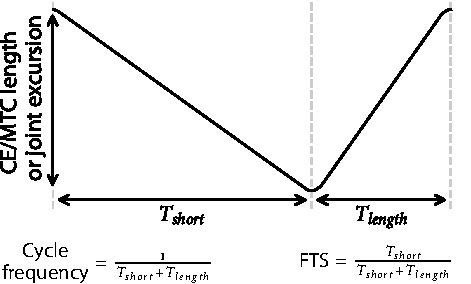
\includegraphics[keepaspectratio]{../figures/i_ssc_parameterisation.pdf}}

}

\caption{\label{fig-i-ssc-parameterisation}\textbf{Parameterisation of
stretch-shortening cycles.} \(T_{short}\) and \(T_{length}\) denote the
shortening and lengthening durations. FTS denotes the fraction of the
cycle time spent shortening. In the example shown, the shortening
duration is 65\% of the cycle duration (i.e.~FTS = 0.65).}

\end{figure}%

Although animal studies have provided valuable insights, it remains
unknown how these findings translate to human muscle. For example, is
the optimal FTS for human muscle also in the order of 0.85? Although
similar experiments can, in principle, be designed for human muscle,
inherent differences exist between experiments involving human
participants and experiments on isolated animal muscles. First, MTC
properties can be accurately estimated in animal experiments based on
dedicated experiments (see \citeproc{ref-reuvers_accuracy_2025}{Reuvers
and Kistemaker, 2025}) that are challenging in human experiments
(i.e.~`quick-release' experiments). Second, CE/MTC length is under full
control in animal experiments, whereas in human movement it can only be
imposed at the joint level. As a result, the exact CE/MTC length over
time is uncertain in human experiments due to inter-individual variation
in, for example, tendon compliance and moment arms. Third, stimulation
is also under full control of the experimenter in animal experiments,
but not in human experiments. Despite these differences, it is feasible
to design human experiments in which imposed joint movements are
systematically varied, with participants aiming to maximise AMPO.
Similarly to animal experiments where CE/MTC length is under full
control, an experimental design should be used in which joint angle over
time is fully imposed, such that the behaviour of the participants does
not have any influence on the kinematics (i.e.~knee joint angle over
time). Such an approach allows investigation of the effects of SSC
parameters -- cycle frequency, FTS, and joint excursion -- on maximally
attainable AMPO. Surprisingly, to our knowledge such studies have not
yet been conducted for human muscle -- not even for sinusoidal SSCs.
Consequently, the effect of SSC parameters on the maximally attainable
AMPO in human muscle is currently unknown.

In this study, we examine the influence of SSC parameters on the
maximally attainable AMPO of human \emph{m. quadriceps femoris} during
short-duration, all-out (sprint) conditions. Under such conditions,
performance is determined by the mechanical properties of the MTC.
Hill-type MTC models have been shown to accurately predict mechanical
behaviour under these conditions (e.g.
\citeproc{ref-van_ingen_schenau_simulation_1988}{Ingen Schenau et al.,
1988}; \citeproc{ref-lemaire_comparison_2016}{Lemaire et al., 2016};
\citeproc{ref-reuvers_maximising_2025}{Reuvers et al., 2025};
\citeproc{ref-sandercock_force_1997}{Sandercock and Heckman, 1997};
\citeproc{ref-wakeling_predicting_1999}{Wakeling and Johnston, 1999};
\citeproc{ref-van_zandwijk_twitch_1996}{Zandwijk et al., 1996}). We
therefore combined model predictions with \emph{in vivo} knee
dynamometer experiments. In both the simulations and the experiments,
knee joint angle over time was fully imposed; in other words, the knee
joint kinetics did not influence the knee joint movement. This allowed
us to examine the direct influence of SSC parameters on the maximally
attainable AMPO. The model was used to predict the maximally attainable
AMPO across a wide range of imposed knee joint movements, from which
nine insightful experimental conditions were selected. In the
experiment, knee joint movements were fully imposed by a knee
dynamometer, while participants aimed to maximise AMPO. Measured AMPO
matched the model predictions reasonably well, confirming that the
Hill-type MTC model reliably captures the influence of SSC parameters on
the maximally attainable AMPO. This justified using the model to
systematically examine the overall influence of imposed knee joint
movement on the maximally attainable AMPO of human \emph{m. quadriceps
femoris}.

\section{Methods}\label{methods}

In this study, we examined the influence of imposed SSC parameters --
cycle frequency, FTS, and joint excursion -- on the maximally attainable
AMPO of human \emph{m. quadriceps femoris}. Experiments were combined
with simulations and optimisations using a Hill-type MTC model. Based on
model predictions, we selected one set of conditions expected to yield
similar AMPO despite substantial variations in knee joint movements, and
another set expected to yield large differences in AMPO. In the
experiment, knee joint movements were fully imposed by a dynamometer.
Participants were instructed to maximise AMPO and, for this purpose,
received visual feedback on cumulative mechanical work throughout each
cycle. Measured AMPO was compared with model predictions. After
confirming that measurements closely matched predictions, the model was
used to investigate the overall influence of SSC parameters on the
maximally attainable AMPO of human \emph{m. quadriceps femoris}.

\subsection{Experiment}\label{experiment}

\subsubsection{Participants and ethical
approval}\label{participants-and-ethical-approval}

Approval of the local ethics committee was obtained before the start of
the \emph{in vivo} experiment (VCWE-2016-135). Four male and two female
healthy participants (22.8 ± 2.2 years, mean ± SD), who all signed
informed consent, participated in the experiment.

\subsubsection{Measurement setup}\label{sec-m-setup}

A kinematically driven knee dynamometer (custom made, Vrije
Universiteit, Amsterdam, the Netherlands, see
\citeproc{ref-de_ruiter_fast_2006}{Ruiter et al., 2006}) was used to
fully impose periodic knee joint angle over time. This dynamometer was
capable of imposing large knee joint accelerations and was sufficiently
stiff such that participant behaviour (i.e.~knee joint moment changes)
did not influence the resulting knee joint movement (see Results).
During the experiment, participants sat in the dynamometer with the
trunk, hip, and thigh firmly strapped. The foot was secured to the
dynamometer footplate to fix the ankle joint. The fixed joint and
segment angles were as follows: the hip angle (between trunk and thigh,
0 rad = fully extended) was about 1.2 rad, the ankle angle (between
shank and foot, 0 rad = fully extended) was about 1.2 rad and the thigh
angle (relative to the horizontal) was about 3.3 rad (see
Figure~\ref{fig-m-setup}). The knee joint angle was defined such that 0
rad corresponded to a fully extended knee, while knee joint angle
increased with flexion (see Figure~\ref{fig-m-setup}). Participants
performed the experiment with their preferred leg. The lower leg was
attached to the sliding carriage of the dynamometer just proximal to the
lateral malleolus (see Figure~\ref{fig-m-setup}). To align the knee
joint with the rotation axis of the dynamometer, the lateral epicondyle
was initially used as a proxy for the knee joint axis while the
participant generated a substantial knee extension moment. Next, the
participant actively extended and flexed their knee over the
experimental joint angle range. During this movement, the travel of the
sliding carriage was visually inspected, and the knee joint alignment
was adjusted to minimise carriage displacement. Net knee joint moment
and knee joint angle were measured with a torque sensor (custom made,
Vrije Universiteit, Amsterdam, the Netherlands) and an angle sensor
(custom made, Vrije Universiteit, Amsterdam, the Netherlands) at a
sample rate of 1000 Hz.

Surface EMG of the \emph{m. vastus medialis}, taken as the reference
muscle for \emph{m. quadriceps femoris}, was measured during the AMPO
measurements. In addition, EMG of \emph{m. biceps femoris}, taken as the
reference muscle for the hamstring muscle group, was measured to test
for undesired co-contraction. Bipolar EMG electrodes (Ambu, Ballerup,
Denmark) were placed at an interelectrode distance of 20mm, at 4/5 of
the line originating from the anterior spina iliaca superior to the
joint space in front of the anterior border of the medial ligament and
at 1/2 of the line originating from the ischial tuberosity to the
lateral epicondyle of the tibia for \emph{m. vastus medialis} and
\emph{m. biceps femoris} respectively (SENIAM guidelines,
\citeproc{ref-hermens_development_2000}{Hermens et al., 2000}). EMG
recordings were amplified with a pre-amplifier (9200 EMG, Goodvaerts
Instruments, Kortenhoef, the Netherlands) and collected at a sample rate
of 4000 Hz.

To synchronise the dynamometer and EMG measurement system, a trigger
pulse generated by the dynamometer system was sent to the EMG
measurement system at the start of each measurement. In addition, knee
joint angle was recorded simultaneously by both systems. After
acquisition, the datasets were aligned based on the trigger pulse. To
verify correct synchronisation, the knee joint angle signals recorded by
the two systems were compared. The signals overlapped after alignment
(i.e., maximal cross-correlation occurred at a time shift of 0),
confirming successful time synchronisation between the dynamometer and
EMG recordings. The EMG signals were downsampled from 4000 Hz to 1000
Hz, beingthe sampling rate of the dynamometer system. Before
downsampling, a low-pass anti-aliasing filter with a cut-off frequency
of 500 Hz (dynamometer sample rate divided by 2) was applied to prevent
aliasing artifacts. All subsequent analyses were performed on the
synchronised and downsampled datasets.

\begin{figure}[H]

\centering{

\pandocbounded{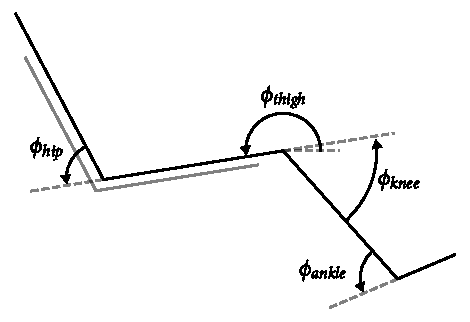
\includegraphics[keepaspectratio]{../figures/m_setup.pdf}}

}

\caption{\label{fig-m-setup}\textbf{The experimental setup.}}

\end{figure}%

\subsubsection{Isometric measurements}\label{sec-m-isom}

The maximally attainable AMPO of participants depends on their maximal
isometric force. Consequently, for a meaningful comparison between the
magnitude of measured AMPO and predicted maximally attainable AMPO, as
well as for meaningful comparisons between participants, we needed an
accurate estimate of each participant's maximal isometric force. To
obtain this estimate, we measured the isometric knee joint moment-angle
relationship for each participant individually. Maximal isometric net
knee joint moment was determined at nine different knee joint angles
equidistantly distributed over a range of knee joint angles between 0.2
rad and 1.8 rad. The order of these measurements was assigned
pseudo-randomly such that they were equally distributed across
participants. Participants were instructed to maximise their net knee
joint moment with their \emph{m. quadriceps femoris} at every knee joint
angle for a period of about five seconds. Participants received
real-time visual feedback about their net knee joint moment on a monitor
which was placed in front of them and were verbally encouraged by the
experimenter. There was a 3-minute rest between each isometric
measurement. At the end of the experiment, the isometric measurements
for the first two knee joint angles were repeated to assess fatigue.

\subsubsection{AMPO measurements}\label{sec-m-ampo}

Experimental conditions for the AMPO measurements were selected based on
simulations using a Hill-type MTC model. Due to limits on knee angular
acceleration, only a subset of combinations of cycle frequency, FTS and
knee joint excursion were experimentally feasible (for details, see
Appendix). Nine experimental conditions that differed in cycle frequency
and FTS at a knee joint excursion of 1.6 rad were used in the experiment
(see Figure~\ref{fig-m-conditions}). One subset of five experimental
conditions was predicted to yield identical maximally attainable AMPO
despite substantial variations in cycle frequency and FTS (0.35A-E;
Figure~\ref{fig-m-conditions}). A second subset of five experimental
conditions was predicted to yield substantial differences in maximally
attainable AMPO due to variations in cycle frequency and FTS (0.20,
0.25, 0.30, 0.35A-E and 0.40; Figure~\ref{fig-m-conditions}). One
experimental condition was shared between both subsets, resulting in
nine unique experimental conditions.

In each experimental condition, 15 consecutive cycles of the respective
knee joint movement were imposed; the participants were instructed to
remain fully relaxed during cycles 1-5 and cycles 11-15 and to maximise
AMPO with their \emph{m. quadriceps femoris} during cycles 6-10.
Throughout all cycles, participants were instructed to relax their
hamstring muscle group to prevent it from producing negative and
positive mechanical work during knee extension and flexion.

\begin{figure}[H]

\centering{

\pandocbounded{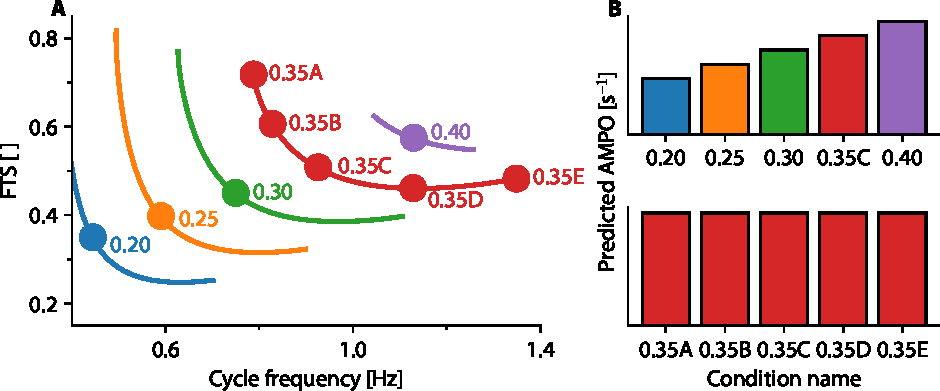
\includegraphics[keepaspectratio]{../figures/m_conditions.pdf}}

}

\caption{\label{fig-m-conditions}\textbf{Predicted maximally attainable
AMPO and experimental conditions.} A) Contour lines depict model-based
predictions of maximally attainable AMPO as a function of cycle
frequency and FTS for a knee joint excursion of 1.6 rad. Contour lines
are only shown for experimentally feasible conditions (due to limits set
on knee joint acceleration; see Appendix). Dots indicate the nine
conditions selected to be evaluated experimentally. B) Barplots of the
same conditions: top, subset predicted to differ in maximally attainable
normalised AMPO (i.e.~0.20, 0.25, 0.30, 0.35C and 0.40); bottom, subset
predicted to yield identical maximally attainable normalised AMPO
(0.35A-E).}

\end{figure}%

The periodic knee joint angle over time was fully imposed by the knee
dynamometer and therefore periodic lengthening and shortening of the MTC
was fully imposed. Consequently, participants could only influence
measured AMPO through their muscle activation. For the predictions
derived with the Hill-type MTC model, muscle activation was optimised
for AMPO (for details, see Methods: Musculoskeletal model). Thus, for a
meaningful comparison between measured AMPO and the predicted maximally
attainable AMPO, it was crucial that participants chose a (near-)optimal
muscle activation of their \emph{m. quadriceps femoris}. Therefore, each
participant practised the nine conditions twice during both practice
days (day 1 and 2) of the experiment. Additionally, all conditions were
performed once at the end of day 3, at which day the isometric
measurements took place. Thus, in total, participants practised each of
the nine conditions five times, equalling 25 active cycles. During both
practice and the actual AMPO measurements, participants received
real-time visual feedback about their cumulative work throughout each
cycle on a monitor and were verbally encouraged by the experimenter to
maximise it.

During the AMPO measurements day (day 4), EMG measurements of \emph{m.
quadriceps femoris} and the hamstring muscle group were taken. At the
start and at the end of the AMPO measurement, participants performed
isometric contractions at a knee joint angle of 1.0 rad: twice for
\emph{m. quadriceps femoris} and twice for the hamstring muscle group in
order to record EMG signals during maximal voluntary contractions
(\(EMG^{MVC}\)) of both muscles, which were later used to normalise EMG
activity during the AMPO measurements (see Methods: Data analysis).
Before the actual measurement, the participants again practised with the
protocol by performing the four most extreme conditions of the
experiment (i.e.~0.20C, 0.35A, 0.35E and 0.40C). To prevent fatigue
during the actual measurements, participants were instructed to perform
these conditions sub-maximally. After this, participants performed the
nine different conditions, from which the first two were repeated at the
end to check for muscle fatigue. As with the isometric measurements, the
order of the AMPO conditions was assigned pseudo-randomly such that they
were equally distributed across participants. There was a 3-minute rest
between each condition.

\subsection{Musculoskeletal model}\label{sec-m-musmodel}

\subsubsection{Description}\label{description}

A planar model consisting of an upper and lower leg connected by a
frictionless hinge joint was used to relate knee joint angle to
muscle-tendon-complex (MTC) length and to relate MTC force to knee joint
moment (for details, see Appendix). The musculoskeletal model did not
contain any knee flexors, as participants were instructed to maximise
AMPO using their knee extensors only. A single Hill-type MTC model was
used to represent the mechanical behaviour of all knee extensors in the
human leg. The formulation of the Hill-type muscle-tendon complex model
has been previously described in full detail
(\citeproc{ref-reuvers_accuracy_2025}{Reuvers and Kistemaker, 2025};
\citeproc{ref-van_soest_contribution_1993}{Soest and Bobbert, 1993}).
Briefly, the Hill-type MTC model included a contractile element (CE)
with a parallel elastic element (PEE) in parallel and a serial elastic
element (SEE) in series with the CE. PEE and SEE were modelled as purely
passive elastic structures, with their force non-linearly dependent on
their length. CE force depended on CE length, CE velocity and active
state. Active state, defined as the relative \(Ca^{2+}\) concentration
bound to troponin C (\citeproc{ref-ebashi_calcium_1968}{Ebashi and Endo,
1968}), depended on free \(Ca^{2+}\) concentration and CE length
(\citeproc{ref-hatze_myocybernetic_1981}{Hatze, 1981}, pp 31-32;
\citeproc{ref-kistemaker_length-dependent_2005}{Kistemaker et al.,
2005}). The free \(Ca^{2+}\) concentration in turn, depended on neural
drive (\(STIM\)) by first-order dynamics. \(STIM\) and the imposed knee
joint angle over time were the model's independent inputs.

\subsubsection{Predictions of maximally attainable
AMPO}\label{sec-m-predictions}

To derive predictions of the maximally attainable AMPO, we used the
musculoskeletal model with parameter values obtained from literature
(see \quartoapptblref{apptbl-parms}). As such, we derived generic
predictions without tuning those to the muscle parameters of the
participants in our experiment. Using the musculoskeletal model, we
imposed periodic knee joint movements in which knee joint angle was
centred around 1.0 rad. We set the knee angular velocities to constant
values that could differ between flexion and extension. We examined a
large number of knee joint movements over a range of cycle frequencies
(0.4-3 Hz, in 0.2 Hz steps), FTS values (0.10-0.90, in 0.05 steps) and
knee joint excursions (0.8-2.0 rad, in 0.1 rad steps). Muscle activation
onset time (i.e.~the time instance at which \(STIM\) switches from 0 to
its maximal value) was chosen at the start of MTC shortening for each
imposed knee joint movement. Muscle activation duration (i.e.~the time
period during which \(STIM\) remains at its maximal value before
returning to 0) was optimised for AMPO using a Nelder-Mead Simplex
method (\citeproc{ref-lagarias_convergence_1998}{Lagarias et al.,
1998}). To ensure periodic behaviour, simulations were run for at least
five cycles and until the difference in MTC force at the beginning and
end of the cycle was less than 0.1\% \(F_{CE}^{max}\). AMPO was
calculated for the last cycle.

\subsection{Data analysis}\label{sec-m-analysis}

The isometric measurements were used to estimate the maximal isometric
force (\(F_{CE}^{max}\)) for each participant individually. The maximal
net knee joint moment was determined for every measured knee joint angle
and was defined as the highest 500 ms average after correcting for
gravitational effects. The moment arm was assumed to be equal for all
participants (i.e.~moment arm = 4.2 cm, see Soest and Casius
(\citeproc{ref-van_soest_which_2000}{2000})). The isometric knee joint
moment-angle relationship of the musculoskeletal model depends on three
parameters: \(F_{CE}^{max}\), \(L_{CE}^{opt}\) (CE optimum length), and
\(L_{SEE}^0\) (SEE slack length). These parameters were estimated
individually for each participant by minimising the sum of squared
differences between the measured isometric net knee joint moment and
those predicted by the musculoskeletal model. This optimisation was
performed using a Nelder-Mead Simplex method
(\citeproc{ref-lagarias_convergence_1998}{Lagarias et al., 1998}).

EMG signals measured during the AMPO measurements were bandpass filtered
using a bidirectional first order Butterworth filter with cut-off
frequencies of 20 and 500 Hz
(\citeproc{ref-butterworth_theory_1930}{Butterworth, 1930}). The EMG
envelope was determined as the absolute value of the Hilbert transformed
EMG signal (\citeproc{ref-hilbert_grundzuge_1904}{Hilbert, 1904}).
\(EMG^{MVC}\) values of \emph{m. vastus medialis} and \emph{m. biceps
femoris} were defined as the maximal average value of the EMG envelope
over 500 ms during the isometric contractions at a knee joint angle of
1.0 rad. Measured EMG signals of \emph{m. vastus medialis} and \emph{m.
biceps femoris} during the AMPO measurements were smoothed by a moving
average filter with a window of 100 ms and were normalised by their
\(EMG^{MVC}\) value. The first and last 0.1 seconds of knee extension
were not taken into account for the calculation of the average EMG
values, as EMG values increased and decreased during these time
intervals. Therefore, average EMG values reported were calculated
between a knee joint angle of 0.45 and 1.55 rad.

The knee joint moment measured by the dynamometer during the AMPO
measurements represented the combined contributions of gravity, inertia
(from both the participant's leg+foot and that of the dynamometer),
passive structures, and active muscle force. To estimate the
contribution of gravity, inertia and passive structures, participants
were instructed to remain fully relaxed during the first and last five
cycles of each experimental condition. The knee joint moment recorded
during these passive cycles was assumed to reflect only the net
non-muscular contribution. To isolate the muscular contribution, the
average knee joint moment from passive cycles 2, 3, 4, 12, 13, and 14
was calculated and subtracted from the measured knee joint moment. The
resulting moment, attributed to the moment resulting from muscle force
only, was called the `muscular' knee joint moment (\(M_{mus}\)). AMPO
per individual cycle was calculated by integrating \(M_{mus}\) over knee
joint angle using a trapezoid method, and dividing the result by the
cycle duration.

Measured AMPO and predicted maximally attainable AMPO were normalised in
two different ways. First, we assessed whether the magnitude of measured
AMPO could be adequately predicted. The predicted maximally attainable
AMPO scales linearly with maximal isometric force (\(F_{CE}^{max}\)) and
also depends on CE optimum length (\(L_{CE}^{opt}\)). The sensitivity
for \(L_{CE}^{opt}\) was, however, low: a 10\% reduction in
\(L_{CE}^{opt}\) resulted in only a 3.7 ± 0.3\% decrease in AMPO across
all experimental conditions. We used the product of the generic model
parameter value of \(L_{CE}^{opt}\) (see \quartoapptblref{apptbl-parms})
and each participant's individually estimated \(F_{CE}^{max}\) to
normalise measured AMPO. The predicted maximally attainable AMPO was
normalised to the generic model parameter values of \(L_{CE}^{opt}\) and
\(F_{CE}^{max}\). Second, we evaluated how well differences in AMPO
between experimental conditions were predicted. For each subject, the
mean (\(\mu\)) and standard deviation (\(\sigma\)) of measured AMPO
across all experimental conditions were calculated, and individual
condition values were transformed into z-scores for each condition
(denoted by the subscript \emph{i}):

\begin{equation}\protect\phantomsection\label{eq-rmtc}{
z_i = \frac{AMPO_i - \mu}{\sigma}
}\end{equation}

This procedure removed the influence of all potential errors affecting
the magnitude of measured AMPO and isolates the relative changes of
AMPO. Model-predicted maximally attainable AMPO values were similarly
transformed into z-scores, allowing a direct comparison between the
measured and predicted z-scores. Importantly, regardless of the
normalisation method, whether by the product of \(L_{CE}^{opt}\) and
\(F_{CE}^{max}\) or by z-scores, measured AMPO was assessed relative to
the maximally attainable AMPO calculated from the generic model
parameters. Thus, normalised model predictions were based on generic
model parameters obtained from literature.

\section{Results}\label{results}

\subsection{AMPO-scaling factors were successfully
obtained}\label{ampo-scaling-factors-were-successfully-obtained}

All six participants were able to execute the isometric measurements at
all imposed knee joint angles. To test for fatigue, the first two knee
joint angles were repeated at the end of the isometric measurements. The
maximal knee joint moment was 6.6 ± 5.9\% lower for the last two
measurements compared to the first two measurements, averaged over all
participants and the two repeated measurements. The normalised root mean
square difference between measured and predicted isometric net knee
joint moments was 5.1 ± 2.4\% on average. Variance in the estimated
values of \(L_{CE}^{opt}\) and \(L_{SEE}^0\) between participants was
low (Table~\ref{tbl-r-muspar}). A representative example of the measured
and modelled maximal isometric knee joint moment as a function of knee
joint angle is depicted in Figure~\ref{fig-r-te-isometric}.

\begin{figure}[H]

\centering{

\pandocbounded{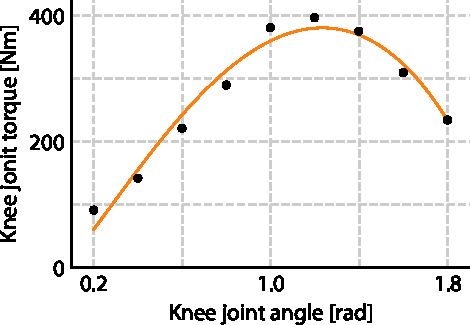
\includegraphics[keepaspectratio]{../figures/r_te_isometric.pdf}}

}

\caption{\label{fig-r-te-isometric}\textbf{Representative example of
maximal isometric knee joint moment as a function of knee joint angle,
shown for participant 5.} Maximal knee joint moment was measured (black
dots) and used to estimate \(L_{SEE}^0\), \(L_{CE}^{opt}\) and
\(F_{CE}^{max}\). The resulting maximal isometric knee joint moment of
the musculoskeletal model is depicted by the orange line.}

\end{figure}%

\begin{table}[H]

\caption{\label{tbl-r-muspar}Estimated parameter values for each
individual participant.}

\centering{

\begin{tabular}{|l|c|c|c|c|} \hline
 \bfseries Participant & $\bm{F_{CE}^{max}}$ [N] & $\bm{L_{CE}^{opt}}$ [cm] & $\bm{L_{SEE}^{0}}$ [cm] & \bfseries RMSD [\%] \\ \hline
1 & 4400 & 8.6 & 17 & 7.3 \\ \hline
2 & 5100 & 9.9 & 15 & 6.9 \\ \hline
3 & 5600 & 8.7 & 17 & 5.8 \\ \hline
4 & 6800 & 8.6 & 16 & 4.1 \\ \hline
5 & 9200 & 7.4 & 18 & 4.7 \\ \hline
6 & 8500 & 8.8 & 16 & 2.9 \\ \hline
AVG±SD & 6600 $\pm$ 1700 & 8.7 $\pm$ 0.7 & 17 $\pm$ 1 & 5.3 $\pm$ 1.6 \\ \hline
\end{tabular}\break\hfill\footnotesize{$F_{CE}^{max}$, $L_{CE}^{opt}$ and $L_{SEE}^{0}$ were estimated from the isometric measurements for each participant individually. The root mean square difference (RMSD) was normalised by the individual maximal predicted knee joint moment, which is the product of $F_{CE}^{max}$ and the moment arm of \textit{m. quadriceps femoris.}}

}

\end{table}%

\subsection{Knee joint movements were successfully
imposed}\label{knee-joint-movements-were-successfully-imposed}

\begin{Shaded}
\begin{Highlighting}[]
\CommentTok{\# \%\% [markdown]}
\CommentTok{\# {-}{-}{-}}
\CommentTok{\# title: Analyse imposed knee joint movements}
\CommentTok{\# {-}{-}{-}}

\CommentTok{\# \%\% [markdown]}
\CommentTok{"""}
\CommentTok{The analysis of this page corresponds to the section \textquotesingle{}Knee joint movements}
\CommentTok{were succesfuly imposed\textquotesingle{}.}

\CommentTok{Specifically, the following steps were taken:}

\CommentTok{{-}   Load condition information (cycle frequency, fraction of time spent shortening) from CSV.}
\CommentTok{{-}   Loop over each participant and condition:}
\CommentTok{    {-}   Load preprocessed AMPO measurement data (day 4).}
\CommentTok{    {-}   Extract relevant columns: time, knee angle (phi), torque, EMG, phase.}
\CommentTok{    {-}   Segment the time and angle data into cycles, extension, and flexion phases.}
\CommentTok{    {-}   Calculate extension time, flexion time, maximum and minimum angles for each cycle.}
\CommentTok{    {-}   Compute the expected theoretical knee angle trajectory for each cycle.}
\CommentTok{    {-}   Compute root mean square difference (RMSD) between measured and theoretical trajectories.}
\CommentTok{{-}   Compute RMSD statistics across participants, conditions, and cycles.}
\CommentTok{{-}   Calculate differences between measured and expected extension/flexion times.}
\CommentTok{{-}   Calculate differences in range of motion (ROM) between measured and theoretical angles.}

\CommentTok{Custom functions used:}

\CommentTok{{-}   \textasciigrave{}helpers.segments\_to\_list(time, phase, segment\_type, cycle\_indices)\textasciigrave{}}
\CommentTok{    : Segments the continuous time series data into lists of individual cycles, extension, or flexion phases.}
\CommentTok{{-}   \textasciigrave{}trajectories.dino(time\_vec, cf, fts, kje, phi\_avg, acc, first\_contr)\textasciigrave{} }
\CommentTok{    : Computes knee angle over time for the dynamometer based on SSC parameters.}
\CommentTok{{-}   \textasciigrave{}stats.rmse(signal1, signal2)\textasciigrave{}}
\CommentTok{    : computes root{-}mean{-}square error between signals.}
\CommentTok{    }
\CommentTok{"""}

\CommentTok{\# \%\% [markdown]}
\CommentTok{"""}
\CommentTok{\#\# Load packages \& set directories}
\CommentTok{"""}

\CommentTok{\#\%\% Load packages}
\ImportTok{import}\NormalTok{ os}
\ImportTok{import}\NormalTok{ sys}
\ImportTok{import}\NormalTok{ pandas }\ImportTok{as}\NormalTok{ pd}
\ImportTok{import}\NormalTok{ numpy }\ImportTok{as}\NormalTok{ np}
\ImportTok{from}\NormalTok{ pathlib }\ImportTok{import}\NormalTok{ Path}

\CommentTok{\# Set directories}
\NormalTok{cwd }\OperatorTok{=}\NormalTok{ Path.cwd()}
\NormalTok{baseDir }\OperatorTok{=}\NormalTok{ cwd.parent}
\NormalTok{dataDir }\OperatorTok{=}\NormalTok{ baseDir }\OperatorTok{/} \StringTok{\textquotesingle{}data\textquotesingle{}}
\NormalTok{funcDir }\OperatorTok{=}\NormalTok{ baseDir }\OperatorTok{/} \StringTok{\textquotesingle{}analysis\textquotesingle{}} \OperatorTok{/} \StringTok{\textquotesingle{}functions\textquotesingle{}}
\NormalTok{sys.path.append(}\BuiltInTok{str}\NormalTok{(funcDir))}

\CommentTok{\# Import custom functions for data processing}
\ImportTok{import}\NormalTok{ helpers, stats, trajectories}

\CommentTok{\# \%\% [markdown]}
\CommentTok{"""}
\CommentTok{\#\# Compute variables for each participant and condition}
\CommentTok{"""}

\CommentTok{\#\%\% Compute variables for each participant and condition}
\CommentTok{\# Load conditions data from CSV file}
\NormalTok{data }\OperatorTok{=}\NormalTok{ pd.read\_csv(os.path.join(dataDir, }\StringTok{\textquotesingle{}conditions.csv\textquotesingle{}}\NormalTok{), sep}\OperatorTok{=}\StringTok{\textquotesingle{},\textquotesingle{}}\NormalTok{, header}\OperatorTok{=}\VariableTok{None}\NormalTok{).to\_numpy()}

\CommentTok{\# Define condition names}
\NormalTok{condNames }\OperatorTok{=}\NormalTok{ [}\StringTok{\textquotesingle{}0.40\textquotesingle{}}\NormalTok{, }\StringTok{\textquotesingle{}0.35C\textquotesingle{}}\NormalTok{, }\StringTok{\textquotesingle{}0.30\textquotesingle{}}\NormalTok{, }\StringTok{\textquotesingle{}0.25\textquotesingle{}}\NormalTok{, }\StringTok{\textquotesingle{}0.20\textquotesingle{}}\NormalTok{, }\StringTok{\textquotesingle{}0.35A\textquotesingle{}}\NormalTok{, }\StringTok{\textquotesingle{}0.35B\textquotesingle{}}\NormalTok{, }\StringTok{\textquotesingle{}0.35D\textquotesingle{}}\NormalTok{, }\StringTok{\textquotesingle{}0.35E\textquotesingle{}}\NormalTok{]}

\CommentTok{\# Extract condition data for cycle frequencies (cf) and flexion time (fts)}
\NormalTok{cf }\OperatorTok{=}\NormalTok{ data[}\DecValTok{1}\NormalTok{].astype(}\BuiltInTok{float}\NormalTok{)}
\NormalTok{fts }\OperatorTok{=}\NormalTok{ data[}\DecValTok{2}\NormalTok{].astype(}\BuiltInTok{float}\NormalTok{)}

\CommentTok{\# Calculate the expected extension and flexion times per condition}
\NormalTok{TextCond }\OperatorTok{=}\NormalTok{ fts }\OperatorTok{/}\NormalTok{ cf  }\CommentTok{\# Extension time}
\NormalTok{TflxCond }\OperatorTok{=}\NormalTok{ (}\DecValTok{1} \OperatorTok{{-}}\NormalTok{ fts) }\OperatorTok{/}\NormalTok{ cf  }\CommentTok{\# Flexion time}

\CommentTok{\# Define maximum and minimum knee angles for conditions}
\NormalTok{phiMaxCond }\OperatorTok{=} \FloatTok{1.8}  \CommentTok{\# Max knee angle (radians)}
\NormalTok{phiMinCond }\OperatorTok{=} \FloatTok{0.2}  \CommentTok{\# Min knee angle (radians)}

\CommentTok{\# List of participants}
\NormalTok{pps }\OperatorTok{=}\NormalTok{ [}\DecValTok{1}\NormalTok{, }\DecValTok{2}\NormalTok{, }\DecValTok{3}\NormalTok{, }\DecValTok{4}\NormalTok{, }\DecValTok{5}\NormalTok{, }\DecValTok{6}\NormalTok{]}

\CommentTok{\# Initialize matrices for storing processed data}
\NormalTok{Ncycli }\OperatorTok{=} \DecValTok{14}  \CommentTok{\# Number of cycles}
\NormalTok{Text }\OperatorTok{=}\NormalTok{ np.nan }\OperatorTok{*}\NormalTok{ np.zeros((}\BuiltInTok{len}\NormalTok{(pps), }\BuiltInTok{len}\NormalTok{(condNames), Ncycli))}
\NormalTok{Tflx }\OperatorTok{=}\NormalTok{ np.nan }\OperatorTok{*}\NormalTok{ np.zeros((}\BuiltInTok{len}\NormalTok{(pps), }\BuiltInTok{len}\NormalTok{(condNames), Ncycli))}
\NormalTok{phiMax }\OperatorTok{=}\NormalTok{ np.nan }\OperatorTok{*}\NormalTok{ np.zeros((}\BuiltInTok{len}\NormalTok{(pps), }\BuiltInTok{len}\NormalTok{(condNames), Ncycli))}
\NormalTok{phiMin }\OperatorTok{=}\NormalTok{ np.nan }\OperatorTok{*}\NormalTok{ np.zeros((}\BuiltInTok{len}\NormalTok{(pps), }\BuiltInTok{len}\NormalTok{(condNames), Ncycli))}
\NormalTok{rmsd }\OperatorTok{=}\NormalTok{ np.nan }\OperatorTok{*}\NormalTok{ np.zeros((}\BuiltInTok{len}\NormalTok{(pps), }\BuiltInTok{len}\NormalTok{(condNames), Ncycli))}

\NormalTok{day }\OperatorTok{=} \DecValTok{4}  \CommentTok{\# Day of experiment}
\NormalTok{trial }\OperatorTok{=} \DecValTok{1}  \CommentTok{\# Trial number}

\ControlFlowTok{for}\NormalTok{ iPP, pp }\KeywordTok{in} \BuiltInTok{enumerate}\NormalTok{(pps):}
    \CommentTok{\# Define directory for each participant\textquotesingle{}s preprocessed data}
\NormalTok{    dataDirPP }\OperatorTok{=}\NormalTok{ os.path.join(dataDir, }\StringTok{\textquotesingle{}dataExp\textquotesingle{}}\NormalTok{, }\SpecialStringTok{f\textquotesingle{}pp}\SpecialCharTok{\{}\NormalTok{pp}\SpecialCharTok{:02d\}}\SpecialStringTok{\textquotesingle{}}\NormalTok{, }\StringTok{\textquotesingle{}AMPO measurements\textquotesingle{}}\NormalTok{, }\StringTok{\textquotesingle{}\textquotesingle{}}\NormalTok{)}
    
    \ControlFlowTok{for}\NormalTok{ iCond, condName }\KeywordTok{in} \BuiltInTok{enumerate}\NormalTok{(condNames):}
        \CommentTok{\# Define filename for each condition}
\NormalTok{        filename }\OperatorTok{=} \SpecialStringTok{f\textquotesingle{}pp}\SpecialCharTok{\{}\NormalTok{pp}\SpecialCharTok{:02d\}}\SpecialStringTok{\_}\SpecialCharTok{\{}\NormalTok{condName}\SpecialCharTok{\}}\SpecialStringTok{\_t1\textquotesingle{}}
        
        \CommentTok{\# Load the preprocessed data}
\NormalTok{        df }\OperatorTok{=}\NormalTok{ pd.read\_csv(os.path.join(dataDirPP, filename }\OperatorTok{+} \StringTok{\textquotesingle{}.csv\textquotesingle{}}\NormalTok{))}
\NormalTok{        data }\OperatorTok{=}\NormalTok{ df.to\_numpy()}
        
        \CommentTok{\# Extract columns from the data}
\NormalTok{        time, phi, \_, torqueComp, \_, \_, emgQuad, emgHams, phase }\OperatorTok{=}\NormalTok{ data.T[:}\DecValTok{9}\NormalTok{]}

        \CommentTok{\# Process the extension and flexion times using the custom function}
\NormalTok{        mTimeExt }\OperatorTok{=}\NormalTok{ helpers.segments\_to\_list(time, phase, }\StringTok{\textquotesingle{}ext\textquotesingle{}}\NormalTok{, np.arange(}\DecValTok{0}\NormalTok{, }\DecValTok{14}\NormalTok{))}
\NormalTok{        mTimeFlx }\OperatorTok{=}\NormalTok{ helpers.segments\_to\_list(time, phase, }\StringTok{\textquotesingle{}flx\textquotesingle{}}\NormalTok{, np.arange(}\DecValTok{0}\NormalTok{, }\DecValTok{14}\NormalTok{))}
        
\NormalTok{        mTime }\OperatorTok{=}\NormalTok{ helpers.segments\_to\_list(time, phase, }\StringTok{\textquotesingle{}cycle\textquotesingle{}}\NormalTok{, np.arange(}\DecValTok{0}\NormalTok{, }\DecValTok{14}\NormalTok{))}
\NormalTok{        mPhi }\OperatorTok{=}\NormalTok{ helpers.segments\_to\_list(phi, phase, }\StringTok{\textquotesingle{}cycle\textquotesingle{}}\NormalTok{, np.arange(}\DecValTok{0}\NormalTok{, }\DecValTok{14}\NormalTok{))}
\NormalTok{        mPhiExt }\OperatorTok{=}\NormalTok{ helpers.segments\_to\_list(phi, phase, }\StringTok{\textquotesingle{}ext\textquotesingle{}}\NormalTok{, np.arange(}\DecValTok{0}\NormalTok{, }\DecValTok{14}\NormalTok{))}
        
        \CommentTok{\# Calculate extension time, flexion time, max and min angles for each cycle}
        \ControlFlowTok{for}\NormalTok{ iCycle }\KeywordTok{in} \BuiltInTok{range}\NormalTok{(Ncycli):}
\NormalTok{            Text[iPP, iCond, iCycle] }\OperatorTok{=}\NormalTok{ mTimeExt[iCycle][}\OperatorTok{{-}}\DecValTok{1}\NormalTok{] }\OperatorTok{{-}}\NormalTok{ mTimeExt[iCycle][}\DecValTok{0}\NormalTok{]}
\NormalTok{            Tflx[iPP, iCond, iCycle] }\OperatorTok{=}\NormalTok{ mTimeFlx[iCycle][}\OperatorTok{{-}}\DecValTok{1}\NormalTok{] }\OperatorTok{{-}}\NormalTok{ mTimeFlx[iCycle][}\DecValTok{0}\NormalTok{]}
\NormalTok{            phiMax[iPP, iCond, iCycle] }\OperatorTok{=}\NormalTok{ mPhiExt[iCycle].}\BuiltInTok{max}\NormalTok{()}
\NormalTok{            phiMin[iPP, iCond, iCycle] }\OperatorTok{=}\NormalTok{ mPhiExt[iCycle].}\BuiltInTok{min}\NormalTok{()}
            
\NormalTok{            phiTheor }\OperatorTok{=}\NormalTok{ trajectories.dino(mTime[iCycle]}\OperatorTok{{-}}\NormalTok{mTime[iCycle][}\DecValTok{0}\NormalTok{],cf[iCond],fts[iCond],kje}\OperatorTok{=}\FloatTok{1.6}\NormalTok{,phi\_avg}\OperatorTok{=}\FloatTok{1.0}\NormalTok{,acc}\OperatorTok{=}\DecValTok{50}\NormalTok{,first\_contr}\OperatorTok{=}\StringTok{\textquotesingle{}E\textquotesingle{}}\NormalTok{)[}\DecValTok{0}\NormalTok{]}
\NormalTok{            rmsd[iPP, iCond, iCycle] }\OperatorTok{=}\NormalTok{ stats.rmse(mPhi[iCycle],phiTheor)}

\CommentTok{\# Root mean square differences}
\NormalTok{rmsd\_mean }\OperatorTok{=} \SpecialStringTok{f"}\SpecialCharTok{\{}\NormalTok{rmsd}\SpecialCharTok{.}\NormalTok{mean()}\OperatorTok{*}\FloatTok{1e3}\SpecialCharTok{:0.0f\}}\SpecialStringTok{"} \CommentTok{\# [mrad] }
\NormalTok{rmsd\_std  }\OperatorTok{=} \SpecialStringTok{f"}\SpecialCharTok{\{}\NormalTok{rmsd}\SpecialCharTok{.}\NormalTok{std()}\OperatorTok{*}\FloatTok{1e3}\SpecialCharTok{:0.0f\}}\SpecialStringTok{"}  \CommentTok{\# [mrad] }

\CommentTok{\# Output ROM results}
\BuiltInTok{print}\NormalTok{(}\SpecialStringTok{f"RMSD is: }\SpecialCharTok{\{}\NormalTok{rmsd\_mean}\SpecialCharTok{\}}\SpecialStringTok{ ± }\SpecialCharTok{\{}\NormalTok{rmsd\_std}\SpecialCharTok{\}}\SpecialStringTok{ mrad"}\NormalTok{)}

\CommentTok{\# Flexion and Extension Time Differences}
\CommentTok{\# Create matrices for the condition\textquotesingle{}s expected times}
\NormalTok{a }\OperatorTok{=}\NormalTok{ np.repeat([TextCond.T], }\DecValTok{6}\NormalTok{, axis}\OperatorTok{=}\DecValTok{0}\NormalTok{)  }\CommentTok{\# Repeat for each participant}
\NormalTok{b }\OperatorTok{=}\NormalTok{ a[:, :, }\VariableTok{None}\NormalTok{]}
\NormalTok{TextCond }\OperatorTok{=}\NormalTok{ np.repeat(b, Ncycli, axis}\OperatorTok{=}\DecValTok{2}\NormalTok{)}

\NormalTok{a }\OperatorTok{=}\NormalTok{ np.repeat([TflxCond.T], }\DecValTok{6}\NormalTok{, axis}\OperatorTok{=}\DecValTok{0}\NormalTok{)}
\NormalTok{b }\OperatorTok{=}\NormalTok{ a[:, :, }\VariableTok{None}\NormalTok{]}
\NormalTok{TflxCond }\OperatorTok{=}\NormalTok{ np.repeat(b, Ncycli, axis}\OperatorTok{=}\DecValTok{2}\NormalTok{)}

\CommentTok{\# Calculate the mean and standard deviation of time differences}
\NormalTok{Text\_mean }\OperatorTok{=} \SpecialStringTok{f"}\SpecialCharTok{\{}\NormalTok{(Text }\OperatorTok{{-}}\NormalTok{ TextCond)}\SpecialCharTok{.}\NormalTok{mean() }\OperatorTok{*} \FloatTok{1e3}\SpecialCharTok{:0.1f\}}\SpecialStringTok{"}  \CommentTok{\# [ms] mean of extension time difference}
\NormalTok{Text\_std }\OperatorTok{=} \SpecialStringTok{f"}\SpecialCharTok{\{}\NormalTok{(Text }\OperatorTok{{-}}\NormalTok{ TextCond)}\SpecialCharTok{.}\NormalTok{std() }\OperatorTok{*} \FloatTok{1e3}\SpecialCharTok{:0.1f\}}\SpecialStringTok{"}  \CommentTok{\# [ms]  std of extension time difference}
\NormalTok{Tflx\_mean }\OperatorTok{=} \SpecialStringTok{f"}\SpecialCharTok{\{}\NormalTok{(Tflx }\OperatorTok{{-}}\NormalTok{ TflxCond)}\SpecialCharTok{.}\NormalTok{mean() }\OperatorTok{*} \FloatTok{1e3}\SpecialCharTok{:0.1f\}}\SpecialStringTok{"}  \CommentTok{\# [ms]  mean of flexion time difference}
\NormalTok{Tflx\_std }\OperatorTok{=} \SpecialStringTok{f"}\SpecialCharTok{\{}\NormalTok{(Tflx }\OperatorTok{{-}}\NormalTok{ TflxCond)}\SpecialCharTok{.}\NormalTok{std() }\OperatorTok{*} \FloatTok{1e3}\SpecialCharTok{:0.1f\}}\SpecialStringTok{"}  \CommentTok{\# [ms] std of flexion time difference}

\CommentTok{\# Output the results}
\BuiltInTok{print}\NormalTok{(}\SpecialStringTok{f"Difference in extension time (desired {-} measured) is: }\SpecialCharTok{\{}\NormalTok{Text\_mean}\SpecialCharTok{\}}\SpecialStringTok{ ± }\SpecialCharTok{\{}\NormalTok{Text\_std}\SpecialCharTok{\}}\SpecialStringTok{ ms"}\NormalTok{)}
\BuiltInTok{print}\NormalTok{(}\SpecialStringTok{f"Difference in flexion time (desired {-} measured) is: }\SpecialCharTok{\{}\NormalTok{Tflx\_mean}\SpecialCharTok{\}}\SpecialStringTok{ ± }\SpecialCharTok{\{}\NormalTok{Tflx\_std}\SpecialCharTok{\}}\SpecialStringTok{ ms"}\NormalTok{)}

\CommentTok{\# Range of Motion (ROM) Calculation}
\CommentTok{\# Calculate ROM (difference between max and min angles) for each cycle}
\NormalTok{rom\_mean }\OperatorTok{=} \SpecialStringTok{f"}\SpecialCharTok{\{}\NormalTok{((phiMax }\OperatorTok{{-}}\NormalTok{ phiMin) }\OperatorTok{{-}}\NormalTok{ (phiMaxCond }\OperatorTok{{-}}\NormalTok{ phiMinCond))}\SpecialCharTok{.}\NormalTok{mean() }\OperatorTok{*} \FloatTok{1e3}\SpecialCharTok{:0.1f\}}\SpecialStringTok{"} \CommentTok{\# [mrad] ROM mean}
\NormalTok{rom\_std  }\OperatorTok{=} \SpecialStringTok{f"}\SpecialCharTok{\{}\NormalTok{((phiMax }\OperatorTok{{-}}\NormalTok{ phiMin) }\OperatorTok{{-}}\NormalTok{ (phiMaxCond }\OperatorTok{{-}}\NormalTok{ phiMinCond))}\SpecialCharTok{.}\NormalTok{std() }\OperatorTok{*} \FloatTok{1e3}\SpecialCharTok{:0.1f\}}\SpecialStringTok{"}  \CommentTok{\# [mrad] ROM std}

\CommentTok{\# Output ROM results}
\BuiltInTok{print}\NormalTok{(}\SpecialStringTok{f"Difference in range of motion (desired {-} measured) is: }\SpecialCharTok{\{}\NormalTok{rom\_mean}\SpecialCharTok{\}}\SpecialStringTok{ ± }\SpecialCharTok{\{}\NormalTok{rom\_std}\SpecialCharTok{\}}\SpecialStringTok{ mrad"}\NormalTok{)}
\end{Highlighting}
\end{Shaded}

For a meaningful comparison between the measured and predicted maximally
attainable AMPO, it was crucial that the knee dynamometer adequately
imposed the desired knee joint movement of the experimental conditions.
This to ensure that both measured and predicted AMPO were based on
(near-)identical knee joint movements. Averaged across all participants,
conditions and cycles, the sum of squared differences between the
desired and measured knee joint angle was only (7 ± 12) \(\cdot\)
10\textsuperscript{-3} rad. As a result, knee extension lasted only 0.6
± 0.5 ms shorter than desired, and knee flexion lasted 0.6 ± 0.5 ms
shorter than desired. In addition, the difference between maximum and
minimum knee joint angle in the experiment was (0.7 ± 0.2) \(\cdot\)
10\textsuperscript{-3} rad higher than desired, averaged across all
participants, conditions and cycles. Overall, the dynamometer
successfully imposed the desired knee joint movements both when
participants were passive and when they aimed to maximise AMPO.

\subsection{\texorpdfstring{Timing of \emph{m. quadriceps femoris}
activation was
adequate}{Timing of m. quadriceps femoris activation was adequate}}\label{timing-of-m.-quadriceps-femoris-activation-was-adequate}

\begin{Shaded}
\begin{Highlighting}[]
\CommentTok{\# \%\% [markdown]}
\CommentTok{\# {-}{-}{-}}
\CommentTok{\# title: EMG and mechanical work}
\CommentTok{\# {-}{-}{-}}

\CommentTok{\# \%\% [markdown]}
\CommentTok{"""}
\CommentTok{The analysis of this page corresponds to the sections \textquotesingle{}Timing of m. quadriceps }
\CommentTok{femoris activation was adequate\textquotesingle{} \& Mechanical work was achieved almost }
\CommentTok{exclusively during knee extension’.}

\CommentTok{Specifically, the following steps were taken:}

\CommentTok{{-}   Define participants and experimental conditions.}
\CommentTok{{-}   Load preprocessed AMPO measurement data for each participant, condition, and trial.}
\CommentTok{{-}   Segment EMG, torque, and knee angle data into cycles, extension, or flexion phases.}
\CommentTok{{-}   Cut EMG and torque data to a specific knee angle range (phi\_range) for analysis.}
\CommentTok{{-}   Compute mean and standard deviation of quadriceps and hamstring EMG during extension and flexion.}
\CommentTok{{-}   Compute cross{-}correlation between quadriceps and hamstring EMG signals during extension.}
\CommentTok{{-}   Compute absolute mechanical work (Mmus) during flexion over the specified knee angle range.}

\CommentTok{Custom functions used:}

\CommentTok{{-}   \textasciigrave{}helpers.segments\_to\_list(data\_array, phase\_array, part, cycle\_indices)\textasciigrave{}}
\CommentTok{    : Segments time series data (EMG, torque, or angle) into individual cycles or specific movement phases.}
\CommentTok{{-}   \textasciigrave{}helpers.data\_cut(data\_list, phi\_list, phi\_range)\textasciigrave{}}
\CommentTok{    : Restricts data to a given range of knee angles and returns the cut data for analysis.}

\CommentTok{"""}

\CommentTok{\# \%\% [markdown]}
\CommentTok{"""}
\CommentTok{\#\# Load packages \& set directories}
\CommentTok{"""}

\CommentTok{\#\%\% Load packages}
\ImportTok{import}\NormalTok{ sys}
\ImportTok{import}\NormalTok{ numpy }\ImportTok{as}\NormalTok{ np}
\ImportTok{import}\NormalTok{ pandas }\ImportTok{as}\NormalTok{ pd}
\ImportTok{from}\NormalTok{ pathlib }\ImportTok{import}\NormalTok{ Path}

\CommentTok{\# Set directories}
\NormalTok{cwd }\OperatorTok{=}\NormalTok{ Path.cwd()}
\NormalTok{baseDir }\OperatorTok{=}\NormalTok{ cwd.parent}
\NormalTok{dataDir }\OperatorTok{=}\NormalTok{ baseDir }\OperatorTok{/} \StringTok{\textquotesingle{}data\textquotesingle{}}
\NormalTok{funcDir }\OperatorTok{=}\NormalTok{ baseDir }\OperatorTok{/} \StringTok{\textquotesingle{}analysis\textquotesingle{}} \OperatorTok{/} \StringTok{\textquotesingle{}functions\textquotesingle{}}
\NormalTok{sys.path.append(}\BuiltInTok{str}\NormalTok{(funcDir))}

\CommentTok{\# Import custom functions}
\ImportTok{import}\NormalTok{ helpers}

\CommentTok{\# \%\% [markdown]}
\CommentTok{"""}
\CommentTok{\#\# Helper function to load and process data}
\CommentTok{"""}

\CommentTok{\#\%\% Helper function to load and process data}
\KeywordTok{def}\NormalTok{ process\_data\_for\_condition(pp, cond, part }\OperatorTok{=} \StringTok{\textquotesingle{}cycle\textquotesingle{}}\NormalTok{, phi\_range}\OperatorTok{=}\NormalTok{[}\FloatTok{0.45}\NormalTok{, }\FloatTok{1.55}\NormalTok{], trial}\OperatorTok{=}\DecValTok{1}\NormalTok{, iCycles}\OperatorTok{=}\NormalTok{[}\DecValTok{5}\NormalTok{, }\DecValTok{6}\NormalTok{, }\DecValTok{7}\NormalTok{, }\DecValTok{8}\NormalTok{, }\DecValTok{9}\NormalTok{]):}
    \CommentTok{"""}
\CommentTok{    Process data for a given participant (pp) and condition (cond) across multiple cycles.}

\CommentTok{    Parameters:}
\CommentTok{    {-}{-}{-}{-}{-}{-}{-}{-}{-}{-}{-}}
\CommentTok{    pp : int}
\CommentTok{        Participant ID.}
\CommentTok{    cond : str}
\CommentTok{        Condition identifier.}
\CommentTok{    trial : int, optional}
\CommentTok{        Trial number (default is 1).}
\CommentTok{    iCycles : list, optional}
\CommentTok{        List of cycles to process (default is [5, 6, 7, 8, 9]).}

\CommentTok{    Returns:}
\CommentTok{    {-}{-}{-}{-}{-}{-}{-}{-}}
\CommentTok{    emgQuadCut : list}
\CommentTok{        Processed EMG data for quadriceps.}
\CommentTok{    emgHamsCut : list}
\CommentTok{        Processed EMG data for hamstrings.}
\CommentTok{    """}
    \CommentTok{\# Construct file path using pathlib}
\NormalTok{    dataDirPP }\OperatorTok{=}\NormalTok{ dataDir }\OperatorTok{/} \StringTok{\textquotesingle{}dataExp\textquotesingle{}} \OperatorTok{/} \SpecialStringTok{f\textquotesingle{}pp}\SpecialCharTok{\{}\NormalTok{pp}\SpecialCharTok{:02d\}}\SpecialStringTok{\textquotesingle{}} \OperatorTok{/} \StringTok{\textquotesingle{}AMPO measurements\textquotesingle{}}
\NormalTok{    filename }\OperatorTok{=} \SpecialStringTok{f\textquotesingle{}pp}\SpecialCharTok{\{}\NormalTok{pp}\SpecialCharTok{:02d\}}\SpecialStringTok{\_}\SpecialCharTok{\{}\NormalTok{cond}\SpecialCharTok{\}}\SpecialStringTok{\_t}\SpecialCharTok{\{}\NormalTok{trial}\SpecialCharTok{\}}\SpecialStringTok{\textquotesingle{}}
    
    \CommentTok{\# Load the data}
\NormalTok{    df }\OperatorTok{=}\NormalTok{ pd.read\_csv(dataDirPP }\OperatorTok{/}\NormalTok{ (filename }\OperatorTok{+} \StringTok{\textquotesingle{}.csv\textquotesingle{}}\NormalTok{))}
\NormalTok{    data }\OperatorTok{=}\NormalTok{ df.T.to\_numpy()}
    
    \CommentTok{\# Extract relevant data columns}
\NormalTok{    time, phi, \_, torqueComp, \_, \_, emgQuad, emgHams, phase }\OperatorTok{=}\NormalTok{ data}

    \CommentTok{\# Adjust cycles for specific conditions}
    \ControlFlowTok{if}\NormalTok{ pp }\OperatorTok{==} \DecValTok{3} \KeywordTok{and}\NormalTok{ cond }\OperatorTok{==} \StringTok{\textquotesingle{}0.35E\textquotesingle{}}\NormalTok{:}
\NormalTok{        iCycles }\OperatorTok{=}\NormalTok{ [}\DecValTok{6}\NormalTok{, }\DecValTok{7}\NormalTok{, }\DecValTok{8}\NormalTok{, }\DecValTok{9}\NormalTok{, }\DecValTok{10}\NormalTok{]  }\CommentTok{\# For pp3 and cond 0.35E, adjust the cycle indices}

    \CommentTok{\# Extract phase{-}specific data for flexion/extension}
\NormalTok{    mPhi        }\OperatorTok{=}\NormalTok{ helpers.segments\_to\_list(phi, phase, part, iCycles)}
\NormalTok{    mEMGquad    }\OperatorTok{=}\NormalTok{ helpers.segments\_to\_list(emgQuad, phase, part, iCycles)}
\NormalTok{    mEMGhams    }\OperatorTok{=}\NormalTok{ helpers.segments\_to\_list(emgHams, phase, part, iCycles)}
\NormalTok{    mTor        }\OperatorTok{=}\NormalTok{ helpers.segments\_to\_list(torqueComp, phase, part, iCycles)}

    \CommentTok{\# Cut the EMG data within the specified range}
\NormalTok{    emg\_quad\_cut, \_ }\OperatorTok{=}\NormalTok{ helpers.data\_cut(mEMGquad, mPhi, phi\_range)}
\NormalTok{    emg\_hams\_cut, \_ }\OperatorTok{=}\NormalTok{ helpers.data\_cut(mEMGhams, mPhi, phi\_range)}
\NormalTok{    tor\_cut, \_      }\OperatorTok{=}\NormalTok{ helpers.data\_cut(mTor, mPhi, phi\_range) }

    \ControlFlowTok{return}\NormalTok{ emg\_quad\_cut, emg\_hams\_cut, tor\_cut}

\CommentTok{\#\%\% Main loop to process all participants and conditions}
\KeywordTok{def}\NormalTok{ process\_all\_conditions(part }\OperatorTok{=} \StringTok{\textquotesingle{}cycle\textquotesingle{}}\NormalTok{, phi\_range}\OperatorTok{=}\NormalTok{[}\FloatTok{0.45}\NormalTok{, }\FloatTok{1.55}\NormalTok{]):}
    \CommentTok{"""}
\CommentTok{    Process all participants and conditions to calculate data over a certain range of knee angles.}
\CommentTok{    """}
\NormalTok{    pps }\OperatorTok{=}\NormalTok{ [}\DecValTok{1}\NormalTok{, }\DecValTok{2}\NormalTok{, }\DecValTok{3}\NormalTok{, }\DecValTok{4}\NormalTok{, }\DecValTok{5}\NormalTok{, }\DecValTok{6}\NormalTok{]}
\NormalTok{    conds }\OperatorTok{=}\NormalTok{ [}\StringTok{\textquotesingle{}0.40\textquotesingle{}}\NormalTok{, }\StringTok{\textquotesingle{}0.35C\textquotesingle{}}\NormalTok{, }\StringTok{\textquotesingle{}0.30\textquotesingle{}}\NormalTok{, }\StringTok{\textquotesingle{}0.25\textquotesingle{}}\NormalTok{, }\StringTok{\textquotesingle{}0.20\textquotesingle{}}\NormalTok{, }\StringTok{\textquotesingle{}0.35A\textquotesingle{}}\NormalTok{, }\StringTok{\textquotesingle{}0.35B\textquotesingle{}}\NormalTok{, }\StringTok{\textquotesingle{}0.35D\textquotesingle{}}\NormalTok{, }\StringTok{\textquotesingle{}0.35E\textquotesingle{}}\NormalTok{]}
    
    \CommentTok{\# Initialize lists to store the results}
\NormalTok{    emg\_quad\_tot }\OperatorTok{=}\NormalTok{ []}
\NormalTok{    emg\_hams\_tot }\OperatorTok{=}\NormalTok{ []}
\NormalTok{    tor\_tot }\OperatorTok{=}\NormalTok{ []}
    
    \CommentTok{\# Process each condition and participant}
    \ControlFlowTok{for}\NormalTok{ cond }\KeywordTok{in}\NormalTok{ conds:}
        \ControlFlowTok{for}\NormalTok{ pp }\KeywordTok{in}\NormalTok{ pps:}
\NormalTok{            emg\_quad\_cut, emg\_hams\_cut, tor\_cut }\OperatorTok{=}\NormalTok{ process\_data\_for\_condition(pp, cond, part, phi\_range)}

            \CommentTok{\# Append the processed EMG data to the total list}
\NormalTok{            emg\_quad\_tot.extend(emg\_quad\_cut)}
\NormalTok{            emg\_hams\_tot.extend(emg\_hams\_cut)}
\NormalTok{            tor\_tot.extend(tor\_cut)}
            
    \ControlFlowTok{return}\NormalTok{ emg\_quad\_tot, emg\_hams\_tot, tor\_tot}

\CommentTok{\# \%\% [markdown]}
\CommentTok{"""}
\CommentTok{\#\# EMG during extension between phi 0.45{-}1.55}
\CommentTok{"""}

\CommentTok{\#\%\% EMG during extension between phi 0.45{-}1.55}
\NormalTok{emg\_quad\_tot, emg\_hams\_tot }\OperatorTok{=}\NormalTok{ process\_all\_conditions(part}\OperatorTok{=}\StringTok{\textquotesingle{}ext\textquotesingle{}}\NormalTok{, phi\_range}\OperatorTok{=}\NormalTok{[}\FloatTok{0.45}\NormalTok{, }\FloatTok{1.55}\NormalTok{])[}\DecValTok{0}\NormalTok{:}\DecValTok{2}\NormalTok{]}

\NormalTok{emg\_quad\_ext\_mean }\OperatorTok{=} \SpecialStringTok{f"}\SpecialCharTok{\{}\NormalTok{np}\SpecialCharTok{.}\NormalTok{concatenate(emg\_quad\_tot)}\SpecialCharTok{.}\NormalTok{astype(}\BuiltInTok{float}\NormalTok{)}\SpecialCharTok{.}\NormalTok{mean()}\OperatorTok{*}\FloatTok{1e2}\SpecialCharTok{:0.1f\}}\SpecialStringTok{"}
\NormalTok{emg\_quad\_ext\_std  }\OperatorTok{=} \SpecialStringTok{f"}\SpecialCharTok{\{}\NormalTok{np}\SpecialCharTok{.}\NormalTok{concatenate(emg\_quad\_tot)}\SpecialCharTok{.}\NormalTok{astype(}\BuiltInTok{float}\NormalTok{)}\SpecialCharTok{.}\NormalTok{std()}\OperatorTok{*}\FloatTok{1e2}\SpecialCharTok{:0.1f\}}\SpecialStringTok{"}
\NormalTok{emg\_hams\_ext\_mean }\OperatorTok{=} \SpecialStringTok{f"}\SpecialCharTok{\{}\NormalTok{np}\SpecialCharTok{.}\NormalTok{concatenate(emg\_hams\_tot)}\SpecialCharTok{.}\NormalTok{astype(}\BuiltInTok{float}\NormalTok{)}\SpecialCharTok{.}\NormalTok{mean()}\OperatorTok{*}\FloatTok{1e2}\SpecialCharTok{:0.1f\}}\SpecialStringTok{"}
\NormalTok{emg\_hams\_ext\_std  }\OperatorTok{=} \SpecialStringTok{f"}\SpecialCharTok{\{}\NormalTok{np}\SpecialCharTok{.}\NormalTok{concatenate(emg\_hams\_tot)}\SpecialCharTok{.}\NormalTok{astype(}\BuiltInTok{float}\NormalTok{)}\SpecialCharTok{.}\NormalTok{std()}\OperatorTok{*}\FloatTok{1e2}\SpecialCharTok{:0.1f\}}\SpecialStringTok{"}

\CommentTok{\# Calculate and print the mean and standard deviation for both muscles}
\BuiltInTok{print}\NormalTok{(}\StringTok{"Quadriceps EMG during extension (between knee angle 0.45{-}1.55 rad): "} \OperatorTok{+}
      \SpecialStringTok{f"}\SpecialCharTok{\{}\NormalTok{emg\_quad\_ext\_mean}\SpecialCharTok{\}}\SpecialStringTok{ ± }\SpecialCharTok{\{}\NormalTok{emg\_quad\_ext\_std}\SpecialCharTok{\}}\SpecialStringTok{ \%"}\NormalTok{)}
\BuiltInTok{print}\NormalTok{(}\StringTok{"Hamsrings EMG during extension (between knee angle 0.45{-}1.55 rad): "} \OperatorTok{+}
      \SpecialStringTok{f"}\SpecialCharTok{\{}\NormalTok{emg\_hams\_ext\_mean}\SpecialCharTok{\}}\SpecialStringTok{ ± }\SpecialCharTok{\{}\NormalTok{emg\_hams\_ext\_std}\SpecialCharTok{\}}\SpecialStringTok{ \%"}\NormalTok{)}

\CommentTok{\# \%\% [markdown]}
\CommentTok{"""}
\CommentTok{\#\# Cross{-}correlationf EMGs during extension between phi 0.2{-}1.8}
\CommentTok{"""}

\CommentTok{\#\%\% Cross{-}correlationf EMGs during extension between phi 0.2{-}1.8}
\CommentTok{\# Process all conditions and participants with a different phi\_range}
\NormalTok{emg\_quad\_tot, emg\_hams\_tot }\OperatorTok{=}\NormalTok{ process\_all\_conditions(part }\OperatorTok{=} \StringTok{\textquotesingle{}ext\textquotesingle{}}\NormalTok{, phi\_range}\OperatorTok{=}\NormalTok{[}\FloatTok{0.2}\NormalTok{, }\FloatTok{1.8}\NormalTok{])[}\DecValTok{0}\NormalTok{:}\DecValTok{2}\NormalTok{]}

\CommentTok{\# Vectorize cross{-}correlation calculation using numpy}
\NormalTok{xcorr }\OperatorTok{=}\NormalTok{ [}
\NormalTok{    np.corrcoef(np.array(x).astype(}\BuiltInTok{float}\NormalTok{), np.array(y).astype(}\BuiltInTok{float}\NormalTok{))[}\DecValTok{0}\NormalTok{, }\DecValTok{1}\NormalTok{]}
    \ControlFlowTok{for}\NormalTok{ x, y }\KeywordTok{in} \BuiltInTok{zip}\NormalTok{(emg\_quad\_tot, emg\_hams\_tot)}
\NormalTok{]}

\CommentTok{\# nanmean because there is 1 participant 1 condition where EMG was not saved..}
\NormalTok{xcorr\_mean }\OperatorTok{=} \SpecialStringTok{f"}\SpecialCharTok{\{}\NormalTok{np}\SpecialCharTok{.}\NormalTok{nanmean(xcorr)}\SpecialCharTok{:0.2f\}}\SpecialStringTok{"}
\NormalTok{xcorr\_std  }\OperatorTok{=} \SpecialStringTok{f"}\SpecialCharTok{\{}\NormalTok{np}\SpecialCharTok{.}\NormalTok{nanstd(xcorr)}\SpecialCharTok{:0.2f\}}\SpecialStringTok{"}

\CommentTok{\# Calculate and print the mean and standard deviation of cross{-}correlation values}
\BuiltInTok{print}\NormalTok{(}\StringTok{"Cross{-}correlation between quad \& hams EMG is: "} \OperatorTok{+} 
      \SpecialStringTok{f"}\SpecialCharTok{\{}\NormalTok{xcorr\_mean}\SpecialCharTok{\}}\SpecialStringTok{ ± }\SpecialCharTok{\{}\NormalTok{xcorr\_std}\SpecialCharTok{\}}\SpecialStringTok{ \%"}\NormalTok{)}

\CommentTok{\# \%\% [markdown]}
\CommentTok{"""}
\CommentTok{\#\# EMG during flexion between phi 0.45{-}1.55}
\CommentTok{"""}

\CommentTok{\#\%\% EMG during flexion between phi 0.45{-}1.55}
\CommentTok{\# Process all conditions and participants}
\NormalTok{emg\_quad\_tot, emg\_hams\_tot }\OperatorTok{=}\NormalTok{ process\_all\_conditions(part}\OperatorTok{=}\StringTok{\textquotesingle{}flx\textquotesingle{}}\NormalTok{, phi\_range}\OperatorTok{=}\NormalTok{[}\FloatTok{0.45}\NormalTok{, }\FloatTok{1.55}\NormalTok{])[}\DecValTok{0}\NormalTok{:}\DecValTok{2}\NormalTok{]}

\NormalTok{emg\_quad\_flx\_mean }\OperatorTok{=} \SpecialStringTok{f"}\SpecialCharTok{\{}\NormalTok{np}\SpecialCharTok{.}\NormalTok{concatenate(emg\_quad\_tot)}\SpecialCharTok{.}\NormalTok{astype(}\BuiltInTok{float}\NormalTok{)}\SpecialCharTok{.}\NormalTok{mean()}\OperatorTok{*}\FloatTok{1e2}\SpecialCharTok{:0.1f\}}\SpecialStringTok{"}
\NormalTok{emg\_quad\_flx\_std  }\OperatorTok{=} \SpecialStringTok{f"}\SpecialCharTok{\{}\NormalTok{np}\SpecialCharTok{.}\NormalTok{concatenate(emg\_quad\_tot)}\SpecialCharTok{.}\NormalTok{astype(}\BuiltInTok{float}\NormalTok{)}\SpecialCharTok{.}\NormalTok{std()}\OperatorTok{*}\FloatTok{1e2}\SpecialCharTok{:0.1f\}}\SpecialStringTok{"}
\NormalTok{emg\_hams\_flx\_mean }\OperatorTok{=} \SpecialStringTok{f"}\SpecialCharTok{\{}\NormalTok{np}\SpecialCharTok{.}\NormalTok{concatenate(emg\_hams\_tot)}\SpecialCharTok{.}\NormalTok{astype(}\BuiltInTok{float}\NormalTok{)}\SpecialCharTok{.}\NormalTok{mean()}\OperatorTok{*}\FloatTok{1e2}\SpecialCharTok{:0.1f\}}\SpecialStringTok{"}
\NormalTok{emg\_hams\_flx\_std  }\OperatorTok{=} \SpecialStringTok{f"}\SpecialCharTok{\{}\NormalTok{np}\SpecialCharTok{.}\NormalTok{concatenate(emg\_hams\_tot)}\SpecialCharTok{.}\NormalTok{astype(}\BuiltInTok{float}\NormalTok{)}\SpecialCharTok{.}\NormalTok{std()}\OperatorTok{*}\FloatTok{1e2}\SpecialCharTok{:0.1f\}}\SpecialStringTok{"}

\CommentTok{\# Calculate and print the mean and standard deviation for both muscles}
\BuiltInTok{print}\NormalTok{(}\StringTok{"Quadriceps EMG during flexion (between knee angle 0.45{-}1.55 rad): "} \OperatorTok{+}
      \SpecialStringTok{f"}\SpecialCharTok{\{}\NormalTok{emg\_quad\_flx\_mean}\SpecialCharTok{\}}\SpecialStringTok{ ± }\SpecialCharTok{\{}\NormalTok{emg\_quad\_flx\_std}\SpecialCharTok{\}}\SpecialStringTok{ \%"}\NormalTok{)}
\BuiltInTok{print}\NormalTok{(}\StringTok{"Hamsrings EMG during flexion (between knee angle 0.45{-}1.55 rad): "} \OperatorTok{+}
      \SpecialStringTok{f"}\SpecialCharTok{\{}\NormalTok{emg\_hams\_flx\_mean}\SpecialCharTok{\}}\SpecialStringTok{ ± }\SpecialCharTok{\{}\NormalTok{emg\_hams\_flx\_std}\SpecialCharTok{\}}\SpecialStringTok{ \%"}\NormalTok{)}

\CommentTok{\# \%\% [markdown]}
\CommentTok{"""}
\CommentTok{\#\# Absolute Mmus during flexion between phi 0.45{-}1.55}
\CommentTok{"""}

\CommentTok{\#\%\% Absolute Mmus during flexion between phi 0.45{-}1.55}
\CommentTok{\# Process all conditions and participants}
\NormalTok{Mmus\_tot }\OperatorTok{=}\NormalTok{ process\_all\_conditions(part}\OperatorTok{=}\StringTok{\textquotesingle{}flx\textquotesingle{}}\NormalTok{, phi\_range}\OperatorTok{=}\NormalTok{[}\FloatTok{0.45}\NormalTok{, }\FloatTok{1.55}\NormalTok{])[}\DecValTok{2}\NormalTok{]}

\NormalTok{Mmus\_mean }\OperatorTok{=} \SpecialStringTok{f"}\SpecialCharTok{\{}\NormalTok{np}\SpecialCharTok{.}\BuiltInTok{abs}\NormalTok{(np.concatenate(Mmus\_tot).astype(}\BuiltInTok{float}\NormalTok{))}\SpecialCharTok{.}\NormalTok{mean()}\SpecialCharTok{:0.1f\}}\SpecialStringTok{"}
\NormalTok{Mmus\_std }\OperatorTok{=} \SpecialStringTok{f"}\SpecialCharTok{\{}\NormalTok{np}\SpecialCharTok{.}\BuiltInTok{abs}\NormalTok{(np.concatenate(Mmus\_tot).astype(}\BuiltInTok{float}\NormalTok{))}\SpecialCharTok{.}\NormalTok{mean()}\SpecialCharTok{:0.1f\}}\SpecialStringTok{"}

\CommentTok{\# Calculate and print the mean and standard deviation for Mmus}
\BuiltInTok{print}\NormalTok{(}\StringTok{"Mmus flexion (between knee angle 0.45{-}1.55 rad): "} \OperatorTok{+}
      \SpecialStringTok{f"}\SpecialCharTok{\{}\NormalTok{Mmus\_mean}\SpecialCharTok{\}}\SpecialStringTok{ ± }\SpecialCharTok{\{}\NormalTok{Mmus\_std}\SpecialCharTok{\}}\SpecialStringTok{ Nm"}\NormalTok{)}
\end{Highlighting}
\end{Shaded}

EMG values during knee extension averaged over all conditions and
participants were 77.7 ± 31.9\% of \(EMG^{MVC}\) for \emph{m. quadriceps
femoris} and 16.7 ± 12.2\% of \(EMG^{MVC}\) for the hamstring muscle
group, between a knee joint angle of 0.45 and 1.55 rad. There was
substantial interindividual variance in EMG values for both muscles,
while variance in EMG values between conditions within each participant
was small. EMG values of the hamstring muscle group increased just
before the transition from flexion to extension and followed a similar
time course as the EMG of \emph{m. quadriceps femoris} (see
Figure~\ref{fig-r-te-emg}). This was reflected by a correlation
coefficient of 0.76 ± 0.18 between EMG values of \emph{m. quadriceps
femoris} and of the hamstring muscle group, suggesting possible
crosstalk between the two muscle groups. During flexion, EMG values of
the hamstring muscle group were close to zero for all participants and
conditions. EMG values of \emph{m. quadriceps femoris} increased just
before the transition from flexion to extension and were close to zero
around the transition from extension to flexion for all participants and
conditions (see Figure~\ref{fig-r-te-emg}). Consequently, \(M_{mus}\)
rose around the transition from flexion to extension and was close to
zero around the transition from extension to flexion
(Figure~\ref{fig-r-te-kinetics}). Except for occasional delays in the
activation onset of \emph{m. quadriceps femoris} during the first active
cycle (cycle 6), \(M_{mus}\) exhibited little variance between cycles
(see also Figure~\ref{fig-r-kinetics}). In sum, participants were
capable of finding an activation of their \emph{m. quadriceps femoris}
that appeared to be (near-)optimal.

\begin{figure}[H]

\centering{

\pandocbounded{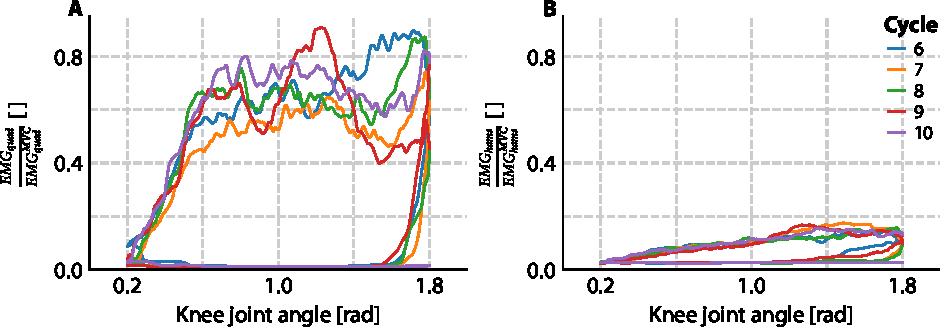
\includegraphics[keepaspectratio]{../figures/r_te_emg.pdf}}

}

\caption{\label{fig-r-te-emg}\textbf{Representative example of measured
EMG, shown for participant 5 under condition 0.35C.} A) EMG of \emph{m.
vastus medialis} normalised by its \(EMG^{MVC}\) value as a function of
knee joint angle. EMG values increased just before the transition from
flexion to extension and were close to zero during flexion, indicating
that the timing of \emph{m. quadriceps femoris} activation of
participants was adequate. B) EMG of the \emph{m. biceps femoris}
normalised by its \(EMG^{MVC}\) value as a function of knee joint angle.
EMG values increased just before the transition from flexion to
extension, following a similar time course as the EMG values of \emph{m.
vastus medialis}, suggesting possible co-contraction. During flexion,
EMG values were close to zero, indicating participants adequately
relaxed their the hamstring muscle group during flexion.}

\end{figure}%

\subsection{Mechanical work was achieved almost exclusively during knee
extension}\label{mechanical-work-was-achieved-almost-exclusively-during-knee-extension}

\begin{Shaded}
\begin{Highlighting}[]
\CommentTok{\# \%\% [markdown]}
\CommentTok{\# {-}{-}{-}}
\CommentTok{\# title: EMG and mechanical work}
\CommentTok{\# {-}{-}{-}}

\CommentTok{\# \%\% [markdown]}
\CommentTok{"""}
\CommentTok{The analysis of this page corresponds to the sections \textquotesingle{}Timing of m. quadriceps }
\CommentTok{femoris activation was adequate\textquotesingle{} \& Mechanical work was achieved almost }
\CommentTok{exclusively during knee extension’.}

\CommentTok{Specifically, the following steps were taken:}

\CommentTok{{-}   Define participants and experimental conditions.}
\CommentTok{{-}   Load preprocessed AMPO measurement data for each participant, condition, and trial.}
\CommentTok{{-}   Segment EMG, torque, and knee angle data into cycles, extension, or flexion phases.}
\CommentTok{{-}   Cut EMG and torque data to a specific knee angle range (phi\_range) for analysis.}
\CommentTok{{-}   Compute mean and standard deviation of quadriceps and hamstring EMG during extension and flexion.}
\CommentTok{{-}   Compute cross{-}correlation between quadriceps and hamstring EMG signals during extension.}
\CommentTok{{-}   Compute absolute mechanical work (Mmus) during flexion over the specified knee angle range.}

\CommentTok{Custom functions used:}

\CommentTok{{-}   \textasciigrave{}helpers.segments\_to\_list(data\_array, phase\_array, part, cycle\_indices)\textasciigrave{}}
\CommentTok{    : Segments time series data (EMG, torque, or angle) into individual cycles or specific movement phases.}
\CommentTok{{-}   \textasciigrave{}helpers.data\_cut(data\_list, phi\_list, phi\_range)\textasciigrave{}}
\CommentTok{    : Restricts data to a given range of knee angles and returns the cut data for analysis.}

\CommentTok{"""}

\CommentTok{\# \%\% [markdown]}
\CommentTok{"""}
\CommentTok{\#\# Load packages \& set directories}
\CommentTok{"""}

\CommentTok{\#\%\% Load packages}
\ImportTok{import}\NormalTok{ sys}
\ImportTok{import}\NormalTok{ numpy }\ImportTok{as}\NormalTok{ np}
\ImportTok{import}\NormalTok{ pandas }\ImportTok{as}\NormalTok{ pd}
\ImportTok{from}\NormalTok{ pathlib }\ImportTok{import}\NormalTok{ Path}

\CommentTok{\# Set directories}
\NormalTok{cwd }\OperatorTok{=}\NormalTok{ Path.cwd()}
\NormalTok{baseDir }\OperatorTok{=}\NormalTok{ cwd.parent}
\NormalTok{dataDir }\OperatorTok{=}\NormalTok{ baseDir }\OperatorTok{/} \StringTok{\textquotesingle{}data\textquotesingle{}}
\NormalTok{funcDir }\OperatorTok{=}\NormalTok{ baseDir }\OperatorTok{/} \StringTok{\textquotesingle{}analysis\textquotesingle{}} \OperatorTok{/} \StringTok{\textquotesingle{}functions\textquotesingle{}}
\NormalTok{sys.path.append(}\BuiltInTok{str}\NormalTok{(funcDir))}

\CommentTok{\# Import custom functions}
\ImportTok{import}\NormalTok{ helpers}

\CommentTok{\# \%\% [markdown]}
\CommentTok{"""}
\CommentTok{\#\# Helper function to load and process data}
\CommentTok{"""}

\CommentTok{\#\%\% Helper function to load and process data}
\KeywordTok{def}\NormalTok{ process\_data\_for\_condition(pp, cond, part }\OperatorTok{=} \StringTok{\textquotesingle{}cycle\textquotesingle{}}\NormalTok{, phi\_range}\OperatorTok{=}\NormalTok{[}\FloatTok{0.45}\NormalTok{, }\FloatTok{1.55}\NormalTok{], trial}\OperatorTok{=}\DecValTok{1}\NormalTok{, iCycles}\OperatorTok{=}\NormalTok{[}\DecValTok{5}\NormalTok{, }\DecValTok{6}\NormalTok{, }\DecValTok{7}\NormalTok{, }\DecValTok{8}\NormalTok{, }\DecValTok{9}\NormalTok{]):}
    \CommentTok{"""}
\CommentTok{    Process data for a given participant (pp) and condition (cond) across multiple cycles.}

\CommentTok{    Parameters:}
\CommentTok{    {-}{-}{-}{-}{-}{-}{-}{-}{-}{-}{-}}
\CommentTok{    pp : int}
\CommentTok{        Participant ID.}
\CommentTok{    cond : str}
\CommentTok{        Condition identifier.}
\CommentTok{    trial : int, optional}
\CommentTok{        Trial number (default is 1).}
\CommentTok{    iCycles : list, optional}
\CommentTok{        List of cycles to process (default is [5, 6, 7, 8, 9]).}

\CommentTok{    Returns:}
\CommentTok{    {-}{-}{-}{-}{-}{-}{-}{-}}
\CommentTok{    emgQuadCut : list}
\CommentTok{        Processed EMG data for quadriceps.}
\CommentTok{    emgHamsCut : list}
\CommentTok{        Processed EMG data for hamstrings.}
\CommentTok{    """}
    \CommentTok{\# Construct file path using pathlib}
\NormalTok{    dataDirPP }\OperatorTok{=}\NormalTok{ dataDir }\OperatorTok{/} \StringTok{\textquotesingle{}dataExp\textquotesingle{}} \OperatorTok{/} \SpecialStringTok{f\textquotesingle{}pp}\SpecialCharTok{\{}\NormalTok{pp}\SpecialCharTok{:02d\}}\SpecialStringTok{\textquotesingle{}} \OperatorTok{/} \StringTok{\textquotesingle{}AMPO measurements\textquotesingle{}}
\NormalTok{    filename }\OperatorTok{=} \SpecialStringTok{f\textquotesingle{}pp}\SpecialCharTok{\{}\NormalTok{pp}\SpecialCharTok{:02d\}}\SpecialStringTok{\_}\SpecialCharTok{\{}\NormalTok{cond}\SpecialCharTok{\}}\SpecialStringTok{\_t}\SpecialCharTok{\{}\NormalTok{trial}\SpecialCharTok{\}}\SpecialStringTok{\textquotesingle{}}
    
    \CommentTok{\# Load the data}
\NormalTok{    df }\OperatorTok{=}\NormalTok{ pd.read\_csv(dataDirPP }\OperatorTok{/}\NormalTok{ (filename }\OperatorTok{+} \StringTok{\textquotesingle{}.csv\textquotesingle{}}\NormalTok{))}
\NormalTok{    data }\OperatorTok{=}\NormalTok{ df.T.to\_numpy()}
    
    \CommentTok{\# Extract relevant data columns}
\NormalTok{    time, phi, \_, torqueComp, \_, \_, emgQuad, emgHams, phase }\OperatorTok{=}\NormalTok{ data}

    \CommentTok{\# Adjust cycles for specific conditions}
    \ControlFlowTok{if}\NormalTok{ pp }\OperatorTok{==} \DecValTok{3} \KeywordTok{and}\NormalTok{ cond }\OperatorTok{==} \StringTok{\textquotesingle{}0.35E\textquotesingle{}}\NormalTok{:}
\NormalTok{        iCycles }\OperatorTok{=}\NormalTok{ [}\DecValTok{6}\NormalTok{, }\DecValTok{7}\NormalTok{, }\DecValTok{8}\NormalTok{, }\DecValTok{9}\NormalTok{, }\DecValTok{10}\NormalTok{]  }\CommentTok{\# For pp3 and cond 0.35E, adjust the cycle indices}

    \CommentTok{\# Extract phase{-}specific data for flexion/extension}
\NormalTok{    mPhi        }\OperatorTok{=}\NormalTok{ helpers.segments\_to\_list(phi, phase, part, iCycles)}
\NormalTok{    mEMGquad    }\OperatorTok{=}\NormalTok{ helpers.segments\_to\_list(emgQuad, phase, part, iCycles)}
\NormalTok{    mEMGhams    }\OperatorTok{=}\NormalTok{ helpers.segments\_to\_list(emgHams, phase, part, iCycles)}
\NormalTok{    mTor        }\OperatorTok{=}\NormalTok{ helpers.segments\_to\_list(torqueComp, phase, part, iCycles)}

    \CommentTok{\# Cut the EMG data within the specified range}
\NormalTok{    emg\_quad\_cut, \_ }\OperatorTok{=}\NormalTok{ helpers.data\_cut(mEMGquad, mPhi, phi\_range)}
\NormalTok{    emg\_hams\_cut, \_ }\OperatorTok{=}\NormalTok{ helpers.data\_cut(mEMGhams, mPhi, phi\_range)}
\NormalTok{    tor\_cut, \_      }\OperatorTok{=}\NormalTok{ helpers.data\_cut(mTor, mPhi, phi\_range) }

    \ControlFlowTok{return}\NormalTok{ emg\_quad\_cut, emg\_hams\_cut, tor\_cut}

\CommentTok{\#\%\% Main loop to process all participants and conditions}
\KeywordTok{def}\NormalTok{ process\_all\_conditions(part }\OperatorTok{=} \StringTok{\textquotesingle{}cycle\textquotesingle{}}\NormalTok{, phi\_range}\OperatorTok{=}\NormalTok{[}\FloatTok{0.45}\NormalTok{, }\FloatTok{1.55}\NormalTok{]):}
    \CommentTok{"""}
\CommentTok{    Process all participants and conditions to calculate data over a certain range of knee angles.}
\CommentTok{    """}
\NormalTok{    pps }\OperatorTok{=}\NormalTok{ [}\DecValTok{1}\NormalTok{, }\DecValTok{2}\NormalTok{, }\DecValTok{3}\NormalTok{, }\DecValTok{4}\NormalTok{, }\DecValTok{5}\NormalTok{, }\DecValTok{6}\NormalTok{]}
\NormalTok{    conds }\OperatorTok{=}\NormalTok{ [}\StringTok{\textquotesingle{}0.40\textquotesingle{}}\NormalTok{, }\StringTok{\textquotesingle{}0.35C\textquotesingle{}}\NormalTok{, }\StringTok{\textquotesingle{}0.30\textquotesingle{}}\NormalTok{, }\StringTok{\textquotesingle{}0.25\textquotesingle{}}\NormalTok{, }\StringTok{\textquotesingle{}0.20\textquotesingle{}}\NormalTok{, }\StringTok{\textquotesingle{}0.35A\textquotesingle{}}\NormalTok{, }\StringTok{\textquotesingle{}0.35B\textquotesingle{}}\NormalTok{, }\StringTok{\textquotesingle{}0.35D\textquotesingle{}}\NormalTok{, }\StringTok{\textquotesingle{}0.35E\textquotesingle{}}\NormalTok{]}
    
    \CommentTok{\# Initialize lists to store the results}
\NormalTok{    emg\_quad\_tot }\OperatorTok{=}\NormalTok{ []}
\NormalTok{    emg\_hams\_tot }\OperatorTok{=}\NormalTok{ []}
\NormalTok{    tor\_tot }\OperatorTok{=}\NormalTok{ []}
    
    \CommentTok{\# Process each condition and participant}
    \ControlFlowTok{for}\NormalTok{ cond }\KeywordTok{in}\NormalTok{ conds:}
        \ControlFlowTok{for}\NormalTok{ pp }\KeywordTok{in}\NormalTok{ pps:}
\NormalTok{            emg\_quad\_cut, emg\_hams\_cut, tor\_cut }\OperatorTok{=}\NormalTok{ process\_data\_for\_condition(pp, cond, part, phi\_range)}

            \CommentTok{\# Append the processed EMG data to the total list}
\NormalTok{            emg\_quad\_tot.extend(emg\_quad\_cut)}
\NormalTok{            emg\_hams\_tot.extend(emg\_hams\_cut)}
\NormalTok{            tor\_tot.extend(tor\_cut)}
            
    \ControlFlowTok{return}\NormalTok{ emg\_quad\_tot, emg\_hams\_tot, tor\_tot}

\CommentTok{\# \%\% [markdown]}
\CommentTok{"""}
\CommentTok{\#\# EMG during extension between phi 0.45{-}1.55}
\CommentTok{"""}

\CommentTok{\#\%\% EMG during extension between phi 0.45{-}1.55}
\NormalTok{emg\_quad\_tot, emg\_hams\_tot }\OperatorTok{=}\NormalTok{ process\_all\_conditions(part}\OperatorTok{=}\StringTok{\textquotesingle{}ext\textquotesingle{}}\NormalTok{, phi\_range}\OperatorTok{=}\NormalTok{[}\FloatTok{0.45}\NormalTok{, }\FloatTok{1.55}\NormalTok{])[}\DecValTok{0}\NormalTok{:}\DecValTok{2}\NormalTok{]}

\NormalTok{emg\_quad\_ext\_mean }\OperatorTok{=} \SpecialStringTok{f"}\SpecialCharTok{\{}\NormalTok{np}\SpecialCharTok{.}\NormalTok{concatenate(emg\_quad\_tot)}\SpecialCharTok{.}\NormalTok{astype(}\BuiltInTok{float}\NormalTok{)}\SpecialCharTok{.}\NormalTok{mean()}\OperatorTok{*}\FloatTok{1e2}\SpecialCharTok{:0.1f\}}\SpecialStringTok{"}
\NormalTok{emg\_quad\_ext\_std  }\OperatorTok{=} \SpecialStringTok{f"}\SpecialCharTok{\{}\NormalTok{np}\SpecialCharTok{.}\NormalTok{concatenate(emg\_quad\_tot)}\SpecialCharTok{.}\NormalTok{astype(}\BuiltInTok{float}\NormalTok{)}\SpecialCharTok{.}\NormalTok{std()}\OperatorTok{*}\FloatTok{1e2}\SpecialCharTok{:0.1f\}}\SpecialStringTok{"}
\NormalTok{emg\_hams\_ext\_mean }\OperatorTok{=} \SpecialStringTok{f"}\SpecialCharTok{\{}\NormalTok{np}\SpecialCharTok{.}\NormalTok{concatenate(emg\_hams\_tot)}\SpecialCharTok{.}\NormalTok{astype(}\BuiltInTok{float}\NormalTok{)}\SpecialCharTok{.}\NormalTok{mean()}\OperatorTok{*}\FloatTok{1e2}\SpecialCharTok{:0.1f\}}\SpecialStringTok{"}
\NormalTok{emg\_hams\_ext\_std  }\OperatorTok{=} \SpecialStringTok{f"}\SpecialCharTok{\{}\NormalTok{np}\SpecialCharTok{.}\NormalTok{concatenate(emg\_hams\_tot)}\SpecialCharTok{.}\NormalTok{astype(}\BuiltInTok{float}\NormalTok{)}\SpecialCharTok{.}\NormalTok{std()}\OperatorTok{*}\FloatTok{1e2}\SpecialCharTok{:0.1f\}}\SpecialStringTok{"}

\CommentTok{\# Calculate and print the mean and standard deviation for both muscles}
\BuiltInTok{print}\NormalTok{(}\StringTok{"Quadriceps EMG during extension (between knee angle 0.45{-}1.55 rad): "} \OperatorTok{+}
      \SpecialStringTok{f"}\SpecialCharTok{\{}\NormalTok{emg\_quad\_ext\_mean}\SpecialCharTok{\}}\SpecialStringTok{ ± }\SpecialCharTok{\{}\NormalTok{emg\_quad\_ext\_std}\SpecialCharTok{\}}\SpecialStringTok{ \%"}\NormalTok{)}
\BuiltInTok{print}\NormalTok{(}\StringTok{"Hamsrings EMG during extension (between knee angle 0.45{-}1.55 rad): "} \OperatorTok{+}
      \SpecialStringTok{f"}\SpecialCharTok{\{}\NormalTok{emg\_hams\_ext\_mean}\SpecialCharTok{\}}\SpecialStringTok{ ± }\SpecialCharTok{\{}\NormalTok{emg\_hams\_ext\_std}\SpecialCharTok{\}}\SpecialStringTok{ \%"}\NormalTok{)}

\CommentTok{\# \%\% [markdown]}
\CommentTok{"""}
\CommentTok{\#\# Cross{-}correlationf EMGs during extension between phi 0.2{-}1.8}
\CommentTok{"""}

\CommentTok{\#\%\% Cross{-}correlationf EMGs during extension between phi 0.2{-}1.8}
\CommentTok{\# Process all conditions and participants with a different phi\_range}
\NormalTok{emg\_quad\_tot, emg\_hams\_tot }\OperatorTok{=}\NormalTok{ process\_all\_conditions(part }\OperatorTok{=} \StringTok{\textquotesingle{}ext\textquotesingle{}}\NormalTok{, phi\_range}\OperatorTok{=}\NormalTok{[}\FloatTok{0.2}\NormalTok{, }\FloatTok{1.8}\NormalTok{])[}\DecValTok{0}\NormalTok{:}\DecValTok{2}\NormalTok{]}

\CommentTok{\# Vectorize cross{-}correlation calculation using numpy}
\NormalTok{xcorr }\OperatorTok{=}\NormalTok{ [}
\NormalTok{    np.corrcoef(np.array(x).astype(}\BuiltInTok{float}\NormalTok{), np.array(y).astype(}\BuiltInTok{float}\NormalTok{))[}\DecValTok{0}\NormalTok{, }\DecValTok{1}\NormalTok{]}
    \ControlFlowTok{for}\NormalTok{ x, y }\KeywordTok{in} \BuiltInTok{zip}\NormalTok{(emg\_quad\_tot, emg\_hams\_tot)}
\NormalTok{]}

\CommentTok{\# nanmean because there is 1 participant 1 condition where EMG was not saved..}
\NormalTok{xcorr\_mean }\OperatorTok{=} \SpecialStringTok{f"}\SpecialCharTok{\{}\NormalTok{np}\SpecialCharTok{.}\NormalTok{nanmean(xcorr)}\SpecialCharTok{:0.2f\}}\SpecialStringTok{"}
\NormalTok{xcorr\_std  }\OperatorTok{=} \SpecialStringTok{f"}\SpecialCharTok{\{}\NormalTok{np}\SpecialCharTok{.}\NormalTok{nanstd(xcorr)}\SpecialCharTok{:0.2f\}}\SpecialStringTok{"}

\CommentTok{\# Calculate and print the mean and standard deviation of cross{-}correlation values}
\BuiltInTok{print}\NormalTok{(}\StringTok{"Cross{-}correlation between quad \& hams EMG is: "} \OperatorTok{+} 
      \SpecialStringTok{f"}\SpecialCharTok{\{}\NormalTok{xcorr\_mean}\SpecialCharTok{\}}\SpecialStringTok{ ± }\SpecialCharTok{\{}\NormalTok{xcorr\_std}\SpecialCharTok{\}}\SpecialStringTok{ \%"}\NormalTok{)}

\CommentTok{\# \%\% [markdown]}
\CommentTok{"""}
\CommentTok{\#\# EMG during flexion between phi 0.45{-}1.55}
\CommentTok{"""}

\CommentTok{\#\%\% EMG during flexion between phi 0.45{-}1.55}
\CommentTok{\# Process all conditions and participants}
\NormalTok{emg\_quad\_tot, emg\_hams\_tot }\OperatorTok{=}\NormalTok{ process\_all\_conditions(part}\OperatorTok{=}\StringTok{\textquotesingle{}flx\textquotesingle{}}\NormalTok{, phi\_range}\OperatorTok{=}\NormalTok{[}\FloatTok{0.45}\NormalTok{, }\FloatTok{1.55}\NormalTok{])[}\DecValTok{0}\NormalTok{:}\DecValTok{2}\NormalTok{]}

\NormalTok{emg\_quad\_flx\_mean }\OperatorTok{=} \SpecialStringTok{f"}\SpecialCharTok{\{}\NormalTok{np}\SpecialCharTok{.}\NormalTok{concatenate(emg\_quad\_tot)}\SpecialCharTok{.}\NormalTok{astype(}\BuiltInTok{float}\NormalTok{)}\SpecialCharTok{.}\NormalTok{mean()}\OperatorTok{*}\FloatTok{1e2}\SpecialCharTok{:0.1f\}}\SpecialStringTok{"}
\NormalTok{emg\_quad\_flx\_std  }\OperatorTok{=} \SpecialStringTok{f"}\SpecialCharTok{\{}\NormalTok{np}\SpecialCharTok{.}\NormalTok{concatenate(emg\_quad\_tot)}\SpecialCharTok{.}\NormalTok{astype(}\BuiltInTok{float}\NormalTok{)}\SpecialCharTok{.}\NormalTok{std()}\OperatorTok{*}\FloatTok{1e2}\SpecialCharTok{:0.1f\}}\SpecialStringTok{"}
\NormalTok{emg\_hams\_flx\_mean }\OperatorTok{=} \SpecialStringTok{f"}\SpecialCharTok{\{}\NormalTok{np}\SpecialCharTok{.}\NormalTok{concatenate(emg\_hams\_tot)}\SpecialCharTok{.}\NormalTok{astype(}\BuiltInTok{float}\NormalTok{)}\SpecialCharTok{.}\NormalTok{mean()}\OperatorTok{*}\FloatTok{1e2}\SpecialCharTok{:0.1f\}}\SpecialStringTok{"}
\NormalTok{emg\_hams\_flx\_std  }\OperatorTok{=} \SpecialStringTok{f"}\SpecialCharTok{\{}\NormalTok{np}\SpecialCharTok{.}\NormalTok{concatenate(emg\_hams\_tot)}\SpecialCharTok{.}\NormalTok{astype(}\BuiltInTok{float}\NormalTok{)}\SpecialCharTok{.}\NormalTok{std()}\OperatorTok{*}\FloatTok{1e2}\SpecialCharTok{:0.1f\}}\SpecialStringTok{"}

\CommentTok{\# Calculate and print the mean and standard deviation for both muscles}
\BuiltInTok{print}\NormalTok{(}\StringTok{"Quadriceps EMG during flexion (between knee angle 0.45{-}1.55 rad): "} \OperatorTok{+}
      \SpecialStringTok{f"}\SpecialCharTok{\{}\NormalTok{emg\_quad\_flx\_mean}\SpecialCharTok{\}}\SpecialStringTok{ ± }\SpecialCharTok{\{}\NormalTok{emg\_quad\_flx\_std}\SpecialCharTok{\}}\SpecialStringTok{ \%"}\NormalTok{)}
\BuiltInTok{print}\NormalTok{(}\StringTok{"Hamsrings EMG during flexion (between knee angle 0.45{-}1.55 rad): "} \OperatorTok{+}
      \SpecialStringTok{f"}\SpecialCharTok{\{}\NormalTok{emg\_hams\_flx\_mean}\SpecialCharTok{\}}\SpecialStringTok{ ± }\SpecialCharTok{\{}\NormalTok{emg\_hams\_flx\_std}\SpecialCharTok{\}}\SpecialStringTok{ \%"}\NormalTok{)}

\CommentTok{\# \%\% [markdown]}
\CommentTok{"""}
\CommentTok{\#\# Absolute Mmus during flexion between phi 0.45{-}1.55}
\CommentTok{"""}

\CommentTok{\#\%\% Absolute Mmus during flexion between phi 0.45{-}1.55}
\CommentTok{\# Process all conditions and participants}
\NormalTok{Mmus\_tot }\OperatorTok{=}\NormalTok{ process\_all\_conditions(part}\OperatorTok{=}\StringTok{\textquotesingle{}flx\textquotesingle{}}\NormalTok{, phi\_range}\OperatorTok{=}\NormalTok{[}\FloatTok{0.45}\NormalTok{, }\FloatTok{1.55}\NormalTok{])[}\DecValTok{2}\NormalTok{]}

\NormalTok{Mmus\_mean }\OperatorTok{=} \SpecialStringTok{f"}\SpecialCharTok{\{}\NormalTok{np}\SpecialCharTok{.}\BuiltInTok{abs}\NormalTok{(np.concatenate(Mmus\_tot).astype(}\BuiltInTok{float}\NormalTok{))}\SpecialCharTok{.}\NormalTok{mean()}\SpecialCharTok{:0.1f\}}\SpecialStringTok{"}
\NormalTok{Mmus\_std }\OperatorTok{=} \SpecialStringTok{f"}\SpecialCharTok{\{}\NormalTok{np}\SpecialCharTok{.}\BuiltInTok{abs}\NormalTok{(np.concatenate(Mmus\_tot).astype(}\BuiltInTok{float}\NormalTok{))}\SpecialCharTok{.}\NormalTok{mean()}\SpecialCharTok{:0.1f\}}\SpecialStringTok{"}

\CommentTok{\# Calculate and print the mean and standard deviation for Mmus}
\BuiltInTok{print}\NormalTok{(}\StringTok{"Mmus flexion (between knee angle 0.45{-}1.55 rad): "} \OperatorTok{+}
      \SpecialStringTok{f"}\SpecialCharTok{\{}\NormalTok{Mmus\_mean}\SpecialCharTok{\}}\SpecialStringTok{ ± }\SpecialCharTok{\{}\NormalTok{Mmus\_std}\SpecialCharTok{\}}\SpecialStringTok{ Nm"}\NormalTok{)}
\end{Highlighting}
\end{Shaded}

Participants were instructed to maximise mechanical work per cycle using
their \emph{m. quadriceps femoris}, while keeping their hamstring muscle
group completely relaxed at all times. Average net knee joint moment
during the passive cycles was subtracted from net knee joint moment
during the active cycles to correct for knee joint moment due to
inertia, gravity and passive structures (see
Figure~\ref{fig-r-te-kinetics}). The resulting knee joint moment
(\(M_{mus}\)) was assumed to be predominantly the result of muscle force
and was, as expected, substantially higher than zero during knee
extension for all participants and conditions. Due to activation and
deactivation delays, \(M_{mus}\) may be above zero just before the
transition from flexion to extension and immediately after the
transition from extension to flexion, in order to maximise AMPO (see
also Figure~\ref{fig-r-kinetics}). Yet, \(M_{mus}\) should be ideally
zero during the middle part of knee flexion. For the active cycle the
absolute value of \(M_{mus}\) was 3.0 ± 3.0 Nm between a knee joint
angle of 0.45 and 1.55 rad (corresponding to 100 ms after and before the
transitions). This minimal \(M_{mus}\) was a result of low activity of
both \emph{m. quadriceps femoris} (2.8 ± 2.7\% of \(EMG^{MVC}\)) and
hamstring muscle group (4.1 ± 4.0\% of \(EMG^{MVC}\)) during the same
time interval. We therefore concluded that participants effectively
relaxed their muscles during knee flexion, such that the net mechanical
work was almost exclusively the result of positive mechanical work
delivered during knee extension (see Table~\ref{tbl-r-mechwork}).

\begin{table}[H]

\caption{\label{tbl-r-mechwork}Positive and negative mechanical work
during knee extension and flexion as a percentage of the net mechanical
work per cycle.}

\centering{

 \begin{tabularx}{\textwidth}{|p{1.0cm}|*{9}{>{\centering\arraybackslash}X|}} \hline
 & \multicolumn{9}{c|}{\textit{Condition}} \\ \hline
 & \bfseries 0.20 & \bfseries 0.25 & \bfseries 0.30 & \bfseries 0.35C & \bfseries 0.40 & \bfseries 0.35A & \bfseries 0.35B & \bfseries 0.35D & \bfseries 0.35E \\ \hline
 \bm{$W_{ext}^{+}$}  & 102.3 $\pm$ 2.5  & 102.2 $\pm$ 2.0  & 103.4 $\pm$ 3.2  & 103.3 $\pm$ 4.3  & 104.2 $\pm$ 3.5  & 104.5 $\pm$ 4.0  & 102.5 $\pm$ 3.6  & 101.9 $\pm$ 4.2  & 100.5 $\pm$ 2.7 \\ \hline 
 \bm{$W_{flex}^{+}$}  & 1.3 $\pm$ 1.2  & 0.9 $\pm$ 0.9  & 1.1 $\pm$ 1.2  & 0.9 $\pm$ 0.7  & 1.4 $\pm$ 1.0  & 1.6 $\pm$ 1.5  & 1.7 $\pm$ 1.2  & 2.6 $\pm$ 1.9  & 3.3 $\pm$ 1.8 \\ \hline 
 \bm{$W_{ext}^{-}$}  & -0.0 $\pm$ 0.1  & -0.0 $\pm$ 0.0  & -0.0 $\pm$ 0.0  & -0.0 $\pm$ 0.0  & -0.0 $\pm$ 0.0  & -0.0 $\pm$ 0.0  & -0.0 $\pm$ 0.0  & -0.0 $\pm$ 0.0  & -0.1 $\pm$ 0.4 \\ \hline 
 \bm{$W_{flex}^{-}$}  & -3.7 $\pm$ 2.2  & -3.1 $\pm$ 2.0  & -4.6 $\pm$ 3.3  & -4.3 $\pm$ 4.1  & -5.6 $\pm$ 3.4  & -6.0 $\pm$ 3.6  & -4.3 $\pm$ 3.0  & -4.7 $\pm$ 4.4  & -3.8 $\pm$ 2.0 \\ \hline 
\end{tabularx}\break\hfill\footnotesize{Positive (+) and negative (-) mechanical work during knee extension (ext) and flexion (flex) were calculated by integrating the instantaneous mechanical power over time, separately for the periods when the instantaneous power was positive (positive work) and negative (negative work) respectively. }

}

\end{table}%

\begin{figure}[H]

\centering{

\pandocbounded{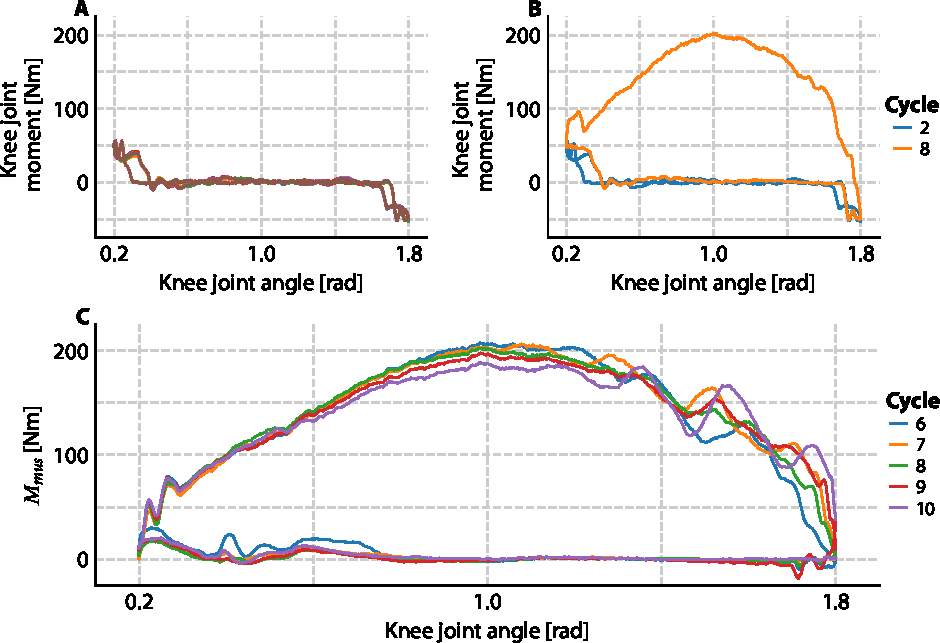
\includegraphics[keepaspectratio]{../figures/r_te_kinetics.pdf}}

}

\caption{\label{fig-r-te-kinetics}\textbf{Representative example of
mechanical behaviour, shown for participant 5 under condition 0.35C.} A)
Knee joint moment during passive cycles. Every individual cycle is
represented by a different coloured line. B) Knee joint moment during
(passive) cycle 2 (blue line) and during (active) cycle 8 (orange line).
C) `Muscular' knee joint moment (\(M_{mus}\)) as a function of knee
joint angle. \(M_{mus}\) was calculated by subtracting average knee
joint moment during the passive cycles from the knee joint moment during
the active cycles (for details Methods). Every individual cycle is
represented by a different coloured line. \(M_{mus}\) was close to zero
during flexion, indicating that the net mechanical work was almost
exclusively the result of mechanical work during extension.}

\end{figure}%

\begin{figure}[H]

\centering{

\pandocbounded{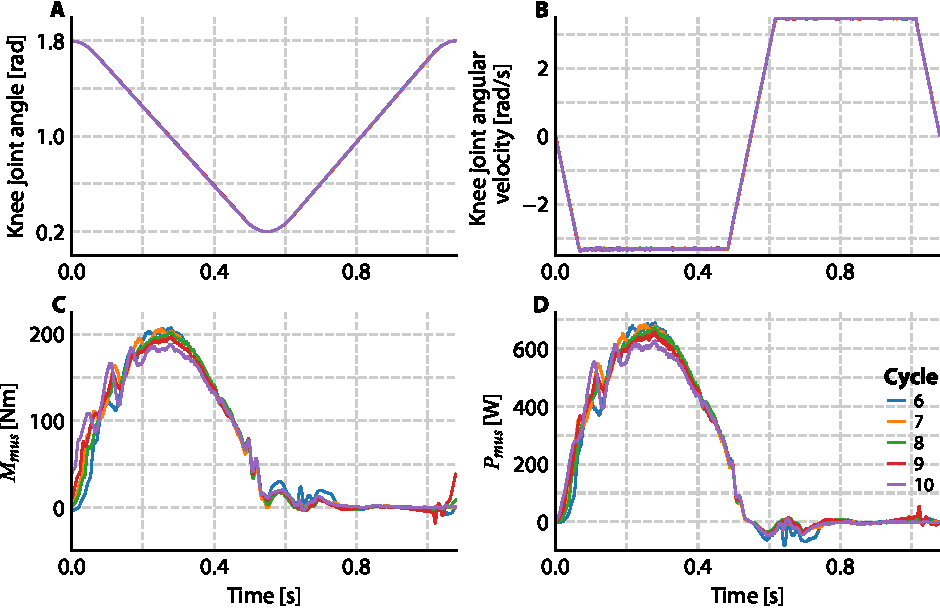
\includegraphics[keepaspectratio]{../figures/r_te_timeseries.pdf}}

}

\caption{\label{fig-r-te-timeseries}\textbf{Representative example of
mechanical behaviour, shown for participant 5 under condition 0.35C.}
Time series are only depicted for the active cycles, where time is set
to zero at the start of knee extension for each cycle. Individual cycles
are represented by a different coloured lines. A) Measured knee joint
angle over time (note that these are indistinguishable between cycles).
B) Measured knee joint angular velocity over time (indistinguishable
between cycles). C) `Muscular' knee joint moment (\(M_{mus}\)) over
time, for cycles 6-10 (see Methods). \(M_{mus}\) was calculated by
subtracting average knee joint moment during the passive cycles from the
knee joint moment during the active cycles (see Methods). D)
Instantaneous `muscular' mechanical power (\(P_{mus}\)) over time, for
cycles 6-10 (see Methods). \(P_{mus}\) was calculated as the product of
\(M_{mus}\) and the measured knee joint angular velocity. Both
\(M_{mus}\) and \(M_{Pus}\) were close to zero during flexion,
indicating that the net mechanical work was almost exclusively the
result of mechanical work during extension.}

\end{figure}%

\newpage{}

\subsection{Measured AMPO closely matched predicted maximally attainable
AMPO}\label{measured-ampo-closely-matched-predicted-maximally-attainable-ampo}

\begin{Shaded}
\begin{Highlighting}[]
\CommentTok{\# \%\% [markdown]}
\CommentTok{\# {-}{-}{-}}
\CommentTok{\# title: Measurements against predictions}
\CommentTok{\# format:}
\CommentTok{\#   html:}
\CommentTok{\#       css: styles.css}
\CommentTok{\# {-}{-}{-}}

\CommentTok{\# \%\% [markdown]}
\CommentTok{"""}
\CommentTok{This script computes the results of the section \textquotesingle{}Measured AMPO closely matched }
\CommentTok{predicted maximally attainable AMPO\textquotesingle{}. }

\CommentTok{For this, it computes:}
\CommentTok{    }
\CommentTok{{-}   Percent difference between the highest and second highest AMPO within one condition}
\CommentTok{{-}   Percent difference between the maximum AMPO of repeated conditions}
\CommentTok{{-}   Measured AMPO per participant and condition}
\CommentTok{{-}   Standardized z{-}scores of predicted and measured AMPO}
\CommentTok{{-}   Linear regression between predicted and measured AMPO (both normalised and z{-}scored)}
\CommentTok{{-}   Squared Pearson correlation coefficient (r²) for both normalised and z{-}scored AMPO}
\CommentTok{    }
\CommentTok{Custom functions used:}
\CommentTok{    }
\CommentTok{{-}   \textasciigrave{}kinetics.compute\_work(phi, torque, phase, part, iCycles)\textasciigrave{}}
\CommentTok{    : Computes net, positive, and negative mechanical work per cycle or per phase}
\CommentTok{{-}   \textasciigrave{}stats.pdiff(value1, value2)\textasciigrave{}}
\CommentTok{    : Computes percent difference between two values}
\CommentTok{{-}   \textasciigrave{}stats.zscore(array, axis)\textasciigrave{}}
\CommentTok{    : Standardizes array to z{-}score along the specified axis}
\CommentTok{{-}   \textasciigrave{}kinetics.compute\_work(phi, torque, phase, part, iCycles)\textasciigrave{}}
\CommentTok{    : Computes net, positive, and negative mechanical work per cycle or per phase}
\CommentTok{"""}

\CommentTok{\# \%\% [markdown]}
\CommentTok{"""}
\CommentTok{\#\# Load packages \& set directories}
\CommentTok{"""}

\CommentTok{\#\%\% Load packages}
\ImportTok{import}\NormalTok{ os, sys}
\ImportTok{import}\NormalTok{ pandas }\ImportTok{as}\NormalTok{ pd}
\ImportTok{import}\NormalTok{ numpy }\ImportTok{as}\NormalTok{ np}
\ImportTok{from}\NormalTok{ scipy }\ImportTok{import}\NormalTok{ stats }\ImportTok{as}\NormalTok{ sp\_stats}
\ImportTok{from}\NormalTok{ pathlib }\ImportTok{import}\NormalTok{ Path}

\CommentTok{\# Set directories}
\NormalTok{cwd }\OperatorTok{=}\NormalTok{ Path.cwd()}
\NormalTok{baseDir }\OperatorTok{=}\NormalTok{ cwd.parent}
\NormalTok{dataDir }\OperatorTok{=}\NormalTok{ baseDir }\OperatorTok{/} \StringTok{\textquotesingle{}data\textquotesingle{}}
\NormalTok{funcDir }\OperatorTok{=}\NormalTok{ baseDir }\OperatorTok{/} \StringTok{\textquotesingle{}analysis\textquotesingle{}} \OperatorTok{/} \StringTok{\textquotesingle{}functions\textquotesingle{}}
\NormalTok{sys.path.append(}\BuiltInTok{str}\NormalTok{(funcDir))}

\ImportTok{import}\NormalTok{ kinetics, stats}

\CommentTok{\# \%\% [markdown]}
\CommentTok{"""}
\CommentTok{\#\# Compute percent difference between the highest and second highest AMPO within one condition}
\CommentTok{"""}

\CommentTok{\#\%\% Highest vs. second highest AMPO}
\NormalTok{p\_max\_vs\_2nd }\OperatorTok{=}\NormalTok{ []}
\NormalTok{ampoDiff }\OperatorTok{=}\NormalTok{ np.nan}\OperatorTok{*}\NormalTok{np.zeros((}\DecValTok{6}\NormalTok{,}\DecValTok{9}\NormalTok{))}
\ControlFlowTok{for}\NormalTok{ iCond, cond }\KeywordTok{in} \BuiltInTok{enumerate}\NormalTok{([}\StringTok{\textquotesingle{}0.40\textquotesingle{}}\NormalTok{, }\StringTok{\textquotesingle{}0.35C\textquotesingle{}}\NormalTok{, }\StringTok{\textquotesingle{}0.30\textquotesingle{}}\NormalTok{, }\StringTok{\textquotesingle{}0.25\textquotesingle{}}\NormalTok{, }\StringTok{\textquotesingle{}0.20\textquotesingle{}}\NormalTok{, }\StringTok{\textquotesingle{}0.35A\textquotesingle{}}\NormalTok{, }\StringTok{\textquotesingle{}0.35B\textquotesingle{}}\NormalTok{, }\StringTok{\textquotesingle{}0.35D\textquotesingle{}}\NormalTok{, }\StringTok{\textquotesingle{}0.35E\textquotesingle{}}\NormalTok{]):}
    \ControlFlowTok{for}\NormalTok{ iPP,pp }\KeywordTok{in} \BuiltInTok{enumerate}\NormalTok{([}\DecValTok{1}\NormalTok{,}\DecValTok{2}\NormalTok{,}\DecValTok{3}\NormalTok{,}\DecValTok{4}\NormalTok{,}\DecValTok{5}\NormalTok{,}\DecValTok{6}\NormalTok{]):}
\NormalTok{        filepath }\OperatorTok{=}\NormalTok{ os.path.join(dataDir,}\StringTok{\textquotesingle{}dataExp\textquotesingle{}}\NormalTok{,}\SpecialStringTok{f\textquotesingle{}pp}\SpecialCharTok{\{}\NormalTok{pp}\SpecialCharTok{:02d\}}\SpecialStringTok{\textquotesingle{}}\NormalTok{,}\StringTok{\textquotesingle{}AMPO measurements\textquotesingle{}}\NormalTok{,}\SpecialStringTok{f\textquotesingle{}pp}\SpecialCharTok{\{}\NormalTok{pp}\SpecialCharTok{:02d\}}\SpecialStringTok{\_}\SpecialCharTok{\{}\NormalTok{cond}\SpecialCharTok{\}}\SpecialStringTok{\_t1.csv\textquotesingle{}}\NormalTok{)}
\NormalTok{        df }\OperatorTok{=}\NormalTok{ pd.read\_csv(filepath)}
\NormalTok{        data }\OperatorTok{=}\NormalTok{ df.T.to\_numpy()}
        
\NormalTok{        time,phi,\_,torqueComp,\_,\_,emgQuad,emgHams,phase }\OperatorTok{=}\NormalTok{ data}
        
\NormalTok{        iCycles }\OperatorTok{=}\NormalTok{ [}\DecValTok{5}\NormalTok{,}\DecValTok{6}\NormalTok{,}\DecValTok{7}\NormalTok{,}\DecValTok{8}\NormalTok{,}\DecValTok{9}\NormalTok{]}
        \ControlFlowTok{if}\NormalTok{ pp }\OperatorTok{==} \DecValTok{3} \KeywordTok{and}\NormalTok{ cond }\OperatorTok{==} \StringTok{\textquotesingle{}0.35E\textquotesingle{}}\NormalTok{:}
\NormalTok{            iCycles }\OperatorTok{=}\NormalTok{ [}\DecValTok{6}\NormalTok{,}\DecValTok{7}\NormalTok{,}\DecValTok{8}\NormalTok{,}\DecValTok{9}\NormalTok{,}\DecValTok{10}\NormalTok{] }\CommentTok{\# for this condition pp3 started one cycle too late!}
\NormalTok{        Wnet,Wpos,Wneg }\OperatorTok{=}\NormalTok{ kinetics.compute\_work(phi,torqueComp,phase,}\StringTok{\textquotesingle{}c\textquotesingle{}}\NormalTok{,iCycles)}
               
\NormalTok{        WnetSort }\OperatorTok{=}\NormalTok{ np.sort(Wnet)}
\NormalTok{        p\_max\_vs\_2nd.append(stats.pdiff(WnetSort[}\OperatorTok{{-}}\DecValTok{2}\NormalTok{],WnetSort[}\OperatorTok{{-}}\DecValTok{1}\NormalTok{]))}
        
\NormalTok{p\_max\_vs\_2nd }\OperatorTok{=}\NormalTok{ np.array(p\_max\_vs\_2nd) }\CommentTok{\# [\%] difference between max. and 2nd max}
\NormalTok{p\_max\_vs\_2nd\_mean }\OperatorTok{=} \SpecialStringTok{f"}\SpecialCharTok{\{}\NormalTok{p\_max\_vs\_2nd}\SpecialCharTok{.}\NormalTok{mean()}\SpecialCharTok{:0.1f\}}\SpecialStringTok{"}  \CommentTok{\# [\%] }
\NormalTok{p\_max\_vs\_2nd\_std  }\OperatorTok{=} \SpecialStringTok{f"}\SpecialCharTok{\{}\NormalTok{p\_max\_vs\_2nd}\SpecialCharTok{.}\NormalTok{std()}\SpecialCharTok{:0.1f\}}\SpecialStringTok{"}  \CommentTok{\# [\%] }

\BuiltInTok{print}\NormalTok{(}\StringTok{"Difference of highest vs. second highest AMPO within one condition is: "} \OperatorTok{+}
      \SpecialStringTok{f"}\SpecialCharTok{\{}\NormalTok{p\_max\_vs\_2nd\_mean}\SpecialCharTok{\}}\SpecialStringTok{ ± }\SpecialCharTok{\{}\NormalTok{p\_max\_vs\_2nd\_std}\SpecialCharTok{\}}\SpecialStringTok{ \%"}\NormalTok{)}

\CommentTok{\# \%\% [markdown]}
\CommentTok{"""}
\CommentTok{\#\# Compute percent difference between the maximum AMPO of repeated conditions}
\CommentTok{"""}

\CommentTok{\#\%\% Difference between max AMPO of regular and repeated condition}
\NormalTok{repConds }\OperatorTok{=}\NormalTok{ np.array([[}\StringTok{\textquotesingle{}0.40\textquotesingle{}}\NormalTok{, }\StringTok{\textquotesingle{}0.35C\textquotesingle{}}\NormalTok{],}
\NormalTok{                    [}\StringTok{\textquotesingle{}0.35C\textquotesingle{}}\NormalTok{, }\StringTok{\textquotesingle{}0.30\textquotesingle{}}\NormalTok{],}
\NormalTok{                    [}\StringTok{\textquotesingle{}0.30\textquotesingle{}}\NormalTok{, }\StringTok{\textquotesingle{}0.25\textquotesingle{}}\NormalTok{],}
\NormalTok{                    [}\StringTok{\textquotesingle{}0.25\textquotesingle{}}\NormalTok{, }\StringTok{\textquotesingle{}0.20\textquotesingle{}}\NormalTok{],}
\NormalTok{                    [}\StringTok{\textquotesingle{}0.20\textquotesingle{}}\NormalTok{, }\StringTok{\textquotesingle{}0.35A\textquotesingle{}}\NormalTok{],}
\NormalTok{                    [}\StringTok{\textquotesingle{}0.35A\textquotesingle{}}\NormalTok{, }\StringTok{\textquotesingle{}0.35B\textquotesingle{}}\NormalTok{]])}

\NormalTok{p\_rep }\OperatorTok{=}\NormalTok{ []}
\NormalTok{iCycles }\OperatorTok{=}\NormalTok{ [}\DecValTok{5}\NormalTok{,}\DecValTok{6}\NormalTok{,}\DecValTok{7}\NormalTok{,}\DecValTok{8}\NormalTok{,}\DecValTok{9}\NormalTok{]}
\ControlFlowTok{for}\NormalTok{ iPP,pp }\KeywordTok{in} \BuiltInTok{enumerate}\NormalTok{([}\DecValTok{1}\NormalTok{,}\DecValTok{2}\NormalTok{,}\DecValTok{3}\NormalTok{,}\DecValTok{4}\NormalTok{,}\DecValTok{5}\NormalTok{,}\DecValTok{6}\NormalTok{]):}
    \ControlFlowTok{for}\NormalTok{ iRep }\KeywordTok{in}\NormalTok{ [}\DecValTok{0}\NormalTok{,}\DecValTok{1}\NormalTok{]:}
\NormalTok{        repCond }\OperatorTok{=}\NormalTok{ repConds[iPP,iRep]}
        
\NormalTok{        filepath }\OperatorTok{=}\NormalTok{ os.path.join(dataDir,}\StringTok{\textquotesingle{}dataExp\textquotesingle{}}\NormalTok{,}\SpecialStringTok{f\textquotesingle{}pp}\SpecialCharTok{\{}\NormalTok{pp}\SpecialCharTok{:02d\}}\SpecialStringTok{\textquotesingle{}}\NormalTok{,}\StringTok{\textquotesingle{}AMPO measurements\textquotesingle{}}\NormalTok{,}\SpecialStringTok{f\textquotesingle{}pp}\SpecialCharTok{\{}\NormalTok{pp}\SpecialCharTok{:02d\}}\SpecialStringTok{\_}\SpecialCharTok{\{}\NormalTok{repCond}\SpecialCharTok{\}}\SpecialStringTok{\_t1.csv\textquotesingle{}}\NormalTok{)}
\NormalTok{        df }\OperatorTok{=}\NormalTok{ pd.read\_csv(filepath)}
\NormalTok{        data }\OperatorTok{=}\NormalTok{ df.T.to\_numpy()}
\NormalTok{        time,phi,\_,torqueComp,\_,\_,emgQuad,emgHams,phase }\OperatorTok{=}\NormalTok{ data}
\NormalTok{        Wnet }\OperatorTok{=}\NormalTok{ kinetics.compute\_work(phi,torqueComp,phase,}\StringTok{\textquotesingle{}c\textquotesingle{}}\NormalTok{,iCycles)[}\DecValTok{0}\NormalTok{]}
        
\NormalTok{        filepath }\OperatorTok{=}\NormalTok{ os.path.join(dataDir,}\StringTok{\textquotesingle{}dataExp\textquotesingle{}}\NormalTok{,}\SpecialStringTok{f\textquotesingle{}pp}\SpecialCharTok{\{}\NormalTok{pp}\SpecialCharTok{:02d\}}\SpecialStringTok{\textquotesingle{}}\NormalTok{,}\StringTok{\textquotesingle{}AMPO measurements\textquotesingle{}}\NormalTok{,}\SpecialStringTok{f\textquotesingle{}pp}\SpecialCharTok{\{}\NormalTok{pp}\SpecialCharTok{:02d\}}\SpecialStringTok{\_}\SpecialCharTok{\{}\NormalTok{repCond}\SpecialCharTok{\}}\SpecialStringTok{\_t2.csv\textquotesingle{}}\NormalTok{)}
\NormalTok{        df }\OperatorTok{=}\NormalTok{ pd.read\_csv(filepath)}
\NormalTok{        data }\OperatorTok{=}\NormalTok{ df.T.to\_numpy()}
\NormalTok{        time,phi,\_,torqueComp,\_,\_,emgQuad,emgHams,phase }\OperatorTok{=}\NormalTok{ data}
\NormalTok{        Wnet\_rep }\OperatorTok{=}\NormalTok{ kinetics.compute\_work(phi,torqueComp,phase,}\StringTok{\textquotesingle{}c\textquotesingle{}}\NormalTok{,iCycles)[}\DecValTok{0}\NormalTok{]  }
    
\NormalTok{        p\_rep.append(stats.pdiff(Wnet\_rep.}\BuiltInTok{max}\NormalTok{(),Wnet.}\BuiltInTok{max}\NormalTok{()))}

\NormalTok{p\_rep }\OperatorTok{=}\NormalTok{ np.array(p\_rep) }\CommentTok{\# [\%] difference between max. and 2nd max}
\NormalTok{p\_rep\_mean }\OperatorTok{=} \SpecialStringTok{f"}\SpecialCharTok{\{}\NormalTok{p\_rep}\SpecialCharTok{.}\NormalTok{mean()}\SpecialCharTok{:0.1f\}}\SpecialStringTok{"}  \CommentTok{\# [\%] }
\NormalTok{p\_rep\_std  }\OperatorTok{=} \SpecialStringTok{f"}\SpecialCharTok{\{}\NormalTok{p\_rep}\SpecialCharTok{.}\NormalTok{std()}\SpecialCharTok{:0.1f\}}\SpecialStringTok{"}  \CommentTok{\# [\%] }

\BuiltInTok{print}\NormalTok{(}\StringTok{"Difference in highest AMPO of repeated conditions is: "} \OperatorTok{+}
      \SpecialStringTok{f"}\SpecialCharTok{\{}\NormalTok{p\_rep\_mean}\SpecialCharTok{\}}\SpecialStringTok{ ± }\SpecialCharTok{\{}\NormalTok{p\_rep\_std}\SpecialCharTok{\}}\SpecialStringTok{ \%"}\NormalTok{)}

\CommentTok{\# \%\% [markdown]}
\CommentTok{"""}
\CommentTok{\#\# Compare measured AMPO against predicted maximally attainable AMPO}
\CommentTok{"""}

\CommentTok{\# \%\% Measured vs. predicted AMPO}
\CommentTok{\# Load conditions}
\NormalTok{data }\OperatorTok{=}\NormalTok{ pd.read\_csv(dataDir }\OperatorTok{/} \StringTok{\textquotesingle{}conditions.csv\textquotesingle{}}\NormalTok{, sep}\OperatorTok{=}\StringTok{\textquotesingle{},\textquotesingle{}}\NormalTok{, header}\OperatorTok{=}\VariableTok{None}\NormalTok{, dtype}\OperatorTok{=}\BuiltInTok{str}\NormalTok{).to\_numpy()}

\CommentTok{\# Set conditions order}
\NormalTok{cond\_names }\OperatorTok{=}\NormalTok{ [}\StringTok{\textquotesingle{}0.20\textquotesingle{}}\NormalTok{, }\StringTok{\textquotesingle{}0.25\textquotesingle{}}\NormalTok{, }\StringTok{\textquotesingle{}0.30\textquotesingle{}}\NormalTok{, }\StringTok{\textquotesingle{}0.35C\textquotesingle{}}\NormalTok{, }\StringTok{\textquotesingle{}0.40\textquotesingle{}}\NormalTok{, }\StringTok{\textquotesingle{}0.35A\textquotesingle{}}\NormalTok{, }\StringTok{\textquotesingle{}0.35B\textquotesingle{}}\NormalTok{, }\StringTok{\textquotesingle{}0.35D\textquotesingle{}}\NormalTok{, }\StringTok{\textquotesingle{}0.35E\textquotesingle{}}\NormalTok{]}

\CommentTok{\# Previously I had a different order, so we need to re{-}order first}
\NormalTok{current\_order }\OperatorTok{=}\NormalTok{ data[}\DecValTok{0}\NormalTok{, :]  }\CommentTok{\# e.g., [\textquotesingle{}0.25\textquotesingle{}, \textquotesingle{}0.20\textquotesingle{}, \textquotesingle{}0.35C\textquotesingle{}, ...]}
\CommentTok{\# Find indices that would reorder to match condNames}
\NormalTok{reorder\_idx }\OperatorTok{=}\NormalTok{ [np.where(current\_order }\OperatorTok{==}\NormalTok{ c)[}\DecValTok{0}\NormalTok{][}\DecValTok{0}\NormalTok{] }\ControlFlowTok{for}\NormalTok{ c }\KeywordTok{in}\NormalTok{ cond\_names]}
\CommentTok{\# Reorder all columns}
\NormalTok{data }\OperatorTok{=}\NormalTok{ data[:, reorder\_idx]}

\NormalTok{c\_cf }\OperatorTok{=}\NormalTok{ data[}\DecValTok{1}\NormalTok{].astype(}\BuiltInTok{float}\NormalTok{)}
\NormalTok{c\_fts }\OperatorTok{=}\NormalTok{ data[}\DecValTok{2}\NormalTok{].astype(}\BuiltInTok{float}\NormalTok{)}
\NormalTok{c\_ampo }\OperatorTok{=}\NormalTok{ data[}\DecValTok{3}\NormalTok{].astype(}\BuiltInTok{float}\NormalTok{)}

\CommentTok{\# Participant info}
\NormalTok{day, trial }\OperatorTok{=} \DecValTok{4}\NormalTok{, }\DecValTok{1}
\NormalTok{pps }\OperatorTok{=}\NormalTok{ [}\DecValTok{1}\NormalTok{, }\DecValTok{2}\NormalTok{, }\DecValTok{3}\NormalTok{, }\DecValTok{4}\NormalTok{, }\DecValTok{5}\NormalTok{, }\DecValTok{6}\NormalTok{]}
\NormalTok{Npp }\OperatorTok{=} \BuiltInTok{len}\NormalTok{(pps)  }\CommentTok{\# number of participants}
\NormalTok{filepath }\OperatorTok{=}\NormalTok{ os.path.join(dataDir,}\StringTok{\textquotesingle{}isometric{-}measurements.csv\textquotesingle{}}\NormalTok{)}
\NormalTok{df }\OperatorTok{=}\NormalTok{ pd.read\_csv(filepath, index\_col}\OperatorTok{=}\DecValTok{0}\NormalTok{)}

\NormalTok{pps }\OperatorTok{=}\NormalTok{ [}\DecValTok{1}\NormalTok{,}\DecValTok{2}\NormalTok{,}\DecValTok{3}\NormalTok{,}\DecValTok{4}\NormalTok{,}\DecValTok{5}\NormalTok{,}\DecValTok{6}\NormalTok{] }\CommentTok{\# participant no.}
\NormalTok{n\_pp }\OperatorTok{=} \BuiltInTok{len}\NormalTok{(pps) }\CommentTok{\# amount of participants}
\NormalTok{fmax }\OperatorTok{=}\NormalTok{ df[}\StringTok{\textquotesingle{}fmax [N]\textquotesingle{}}\NormalTok{].to\_numpy() }\CommentTok{\# [N] est maximal isometric CE force per particiapnt}

\CommentTok{\# Predictions}
\NormalTok{ampo\_pred }\OperatorTok{=}\NormalTok{ np.array([}\FloatTok{0.2}\NormalTok{, }\FloatTok{0.25}\NormalTok{, }\FloatTok{0.3}\NormalTok{, }\FloatTok{0.35}\NormalTok{, }\FloatTok{0.4}\NormalTok{, }\FloatTok{0.35}\NormalTok{, }\FloatTok{0.35}\NormalTok{, }\FloatTok{0.35}\NormalTok{, }\FloatTok{0.35}\NormalTok{])}
\NormalTok{ampo\_pred }\OperatorTok{=}\NormalTok{ np.repeat(ampo\_pred[}\VariableTok{None}\NormalTok{, :], Npp, axis}\OperatorTok{=}\DecValTok{0}\NormalTok{)}

\CommentTok{\# Compute measured AMPO}
\NormalTok{ampo\_exp }\OperatorTok{=}\NormalTok{ np.full((Npp, }\BuiltInTok{len}\NormalTok{(cond\_names)), np.nan)}
\ControlFlowTok{for}\NormalTok{ i\_pp, pp }\KeywordTok{in} \BuiltInTok{enumerate}\NormalTok{(}\BuiltInTok{range}\NormalTok{(}\DecValTok{1}\NormalTok{, Npp }\OperatorTok{+} \DecValTok{1}\NormalTok{)):}
    \ControlFlowTok{for}\NormalTok{ i\_cond, cond }\KeywordTok{in} \BuiltInTok{enumerate}\NormalTok{(cond\_names):}
\NormalTok{        data\_folder }\OperatorTok{=}\NormalTok{ dataDir }\OperatorTok{/} \StringTok{"dataExp"} \OperatorTok{/} \SpecialStringTok{f"pp}\SpecialCharTok{\{}\NormalTok{pp}\SpecialCharTok{:02d\}}\SpecialStringTok{"} \OperatorTok{/} \StringTok{"AMPO measurements"}
\NormalTok{        filename }\OperatorTok{=} \SpecialStringTok{f"pp}\SpecialCharTok{\{}\NormalTok{pp}\SpecialCharTok{:02d\}}\SpecialStringTok{\_}\SpecialCharTok{\{}\NormalTok{cond}\SpecialCharTok{\}}\SpecialStringTok{\_t}\SpecialCharTok{\{}\NormalTok{trial}\SpecialCharTok{\}}\SpecialStringTok{"}

\NormalTok{        df }\OperatorTok{=}\NormalTok{ pd.read\_csv(data\_folder }\OperatorTok{/} \SpecialStringTok{f"}\SpecialCharTok{\{}\NormalTok{filename}\SpecialCharTok{\}}\SpecialStringTok{.csv"}\NormalTok{)}
\NormalTok{        data }\OperatorTok{=}\NormalTok{ df.T.to\_numpy()}
\NormalTok{        \_, phi, \_, torque\_comp, }\OperatorTok{*}\NormalTok{\_ , phase }\OperatorTok{=}\NormalTok{ data[}\DecValTok{0}\NormalTok{:}\DecValTok{9}\NormalTok{]}

        \CommentTok{\# Default cycles}
\NormalTok{        i\_cycles }\OperatorTok{=}\NormalTok{ [}\DecValTok{5}\NormalTok{, }\DecValTok{6}\NormalTok{, }\DecValTok{7}\NormalTok{, }\DecValTok{8}\NormalTok{, }\DecValTok{9}\NormalTok{]}
        \ControlFlowTok{if}\NormalTok{ pp }\OperatorTok{==} \DecValTok{3} \KeywordTok{and}\NormalTok{ cond }\OperatorTok{==} \StringTok{"0.35E"}\NormalTok{:}
\NormalTok{            i\_cycles }\OperatorTok{=}\NormalTok{ [}\DecValTok{6}\NormalTok{, }\DecValTok{7}\NormalTok{, }\DecValTok{8}\NormalTok{, }\DecValTok{9}\NormalTok{, }\DecValTok{10}\NormalTok{]}

        \CommentTok{\# Compute work}
\NormalTok{        Wnet, Wpos, Wneg }\OperatorTok{=}\NormalTok{ kinetics.compute\_work(phi, torque\_comp, phase, part}\OperatorTok{=}\StringTok{"cycle"}\NormalTok{, iCycles}\OperatorTok{=}\NormalTok{i\_cycles)}

        \CommentTok{\# Normalize to participant\textquotesingle{}s max force and convert to AMPO}
\NormalTok{        ampo\_exp[i\_pp, i\_cond] }\OperatorTok{=}\NormalTok{ np.}\BuiltInTok{max}\NormalTok{(Wnet }\OperatorTok{*}\NormalTok{ c\_cf[i\_cond]) }\OperatorTok{/}\NormalTok{ (fmax[i\_pp] }\OperatorTok{*} \FloatTok{0.093}\NormalTok{)}

\CommentTok{\# Compute mean and SEM across participants}
\NormalTok{ampo\_exp\_mean }\OperatorTok{=}\NormalTok{ np.mean(ampo\_exp, axis}\OperatorTok{=}\DecValTok{0}\NormalTok{)}
\NormalTok{ampo\_exp\_sem }\OperatorTok{=}\NormalTok{ np.std(ampo\_exp, axis}\OperatorTok{=}\DecValTok{0}\NormalTok{, ddof}\OperatorTok{=}\DecValTok{1}\NormalTok{) }\OperatorTok{/}\NormalTok{ np.sqrt(Npp)}

\CommentTok{\# Standardize for z{-}score}
\NormalTok{ampo\_pred\_z }\OperatorTok{=}\NormalTok{ stats.zscore(ampo\_exp, axis}\OperatorTok{={-}}\DecValTok{1}\NormalTok{)}
\NormalTok{ampo\_exp\_z }\OperatorTok{=}\NormalTok{ stats.zscore(ampo\_pred, axis}\OperatorTok{={-}}\DecValTok{1}\NormalTok{)}

\CommentTok{\# Linear regressions}
\NormalTok{fit\_norm }\OperatorTok{=}\NormalTok{ sp\_stats.linregress(np.ravel(ampo\_pred), np.ravel(ampo\_exp))}
\NormalTok{fit\_zsco }\OperatorTok{=}\NormalTok{ sp\_stats.linregress(np.ravel(ampo\_pred\_z), np.ravel(ampo\_exp\_z))}

\NormalTok{r2\_norm }\OperatorTok{=} \SpecialStringTok{f"}\SpecialCharTok{\{}\NormalTok{fit\_norm}\SpecialCharTok{.}\NormalTok{rvalue }\OperatorTok{**} \DecValTok{2}\SpecialCharTok{:0.2f\}}\SpecialStringTok{"}
\NormalTok{r2\_zsco }\OperatorTok{=} \SpecialStringTok{f"}\SpecialCharTok{\{}\NormalTok{fit\_zsco}\SpecialCharTok{.}\NormalTok{rvalue }\OperatorTok{**} \DecValTok{2}\SpecialCharTok{:0.2f\}}\SpecialStringTok{"}

\BuiltInTok{print}\NormalTok{(}\SpecialStringTok{f"r² (norm AMPO): }\SpecialCharTok{\{}\NormalTok{r2\_norm}\SpecialCharTok{\}}\SpecialStringTok{"}\NormalTok{)}
\BuiltInTok{print}\NormalTok{(}\SpecialStringTok{f"r² (z{-}scored AMPO): }\SpecialCharTok{\{}\NormalTok{r2\_zsco}\SpecialCharTok{\}}\SpecialStringTok{"}\NormalTok{)}

\CommentTok{\# Measured vs. predicted {-} absolute values (used in discussion)}
\NormalTok{p\_pred\_vs\_exp\_mean }\OperatorTok{=} \SpecialStringTok{f"}\SpecialCharTok{\{}\DecValTok{100} \OperatorTok{+}\NormalTok{ stats}\SpecialCharTok{.}\NormalTok{pdiff(ampo\_exp,ampo\_pred)}\SpecialCharTok{.}\NormalTok{mean()}\SpecialCharTok{:0.0f\}}\SpecialStringTok{"}
\NormalTok{p\_pred\_vs\_exp\_std  }\OperatorTok{=} \SpecialStringTok{f"}\SpecialCharTok{\{}\NormalTok{stats}\SpecialCharTok{.}\NormalTok{pdiff(ampo\_exp,ampo\_pred)}\SpecialCharTok{.}\NormalTok{std()}\SpecialCharTok{:0.0f\}}\SpecialStringTok{"}

\BuiltInTok{print}\NormalTok{(}\SpecialStringTok{f"Measued AMPO is }\SpecialCharTok{\{}\NormalTok{p\_pred\_vs\_exp\_mean}\SpecialCharTok{\}}\SpecialStringTok{ ± }\SpecialCharTok{\{}\NormalTok{p\_pred\_vs\_exp\_std}\SpecialCharTok{\}}\SpecialStringTok{ \% "} \OperatorTok{+}
      \StringTok{"of predicted AMPO"}\NormalTok{)}
\end{Highlighting}
\end{Shaded}

To assess the reliability of AMPO measurements, we examined the
variability of measured AMPO across cycles and repeated conditions.
Averaged across each condition and for each participant, the
second-highest measured AMPO was only -2.4 ± 2.3\% lower than the
highest value, indicating low variance in AMPO between cycles.
Furthermore, in repeated conditions, the highest measured AMPO at the
end of the experiment was just -2.3 ± 4.1\% lower than at the start.
Together, these results indicate that AMPO measurements were consistent
across cycles and throughout the experimental session.

Measured AMPO was compared against the predicted maximally attainable
AMPO. First, AMPO was normalised by the generic value of
\(L_{CE}^{opt}\) and participants' individually estimated
\(F_{CE}^{max}\) (see Methods: Data analysis). As predicted, (1)
measured AMPO differed substantially between conditions 0.20, 0.25,
0.30, 0.35 and 0.40 due to the imposed variations in cycle frequency and
FTS and (2) measured AMPO was almost identical for conditions 0.35A-E,
despite substantial variations in cycle frequency and FTS
(Figure~\ref{fig-r-overview}; Table~\ref{tbl-r-overview}). Overall,
measured AMPO normalised by \(L_{CE}^{opt}\) and participants'
individual \(F_{CE}^{max}\) correlated strongly with predicted maximally
attainable AMPO (r\textsuperscript{2}=0.75). Second, AMPO was normalised
by z-scores of measured and predicted maximally attainable AMPO. This
revealed a very strong correlation between predictions and measurements
(r\textsuperscript{2}=0.95). All in all, measured AMPO was remarkably
close to the predicted maximally attainable AMPO.

\begin{figure}[H]

\centering{

\pandocbounded{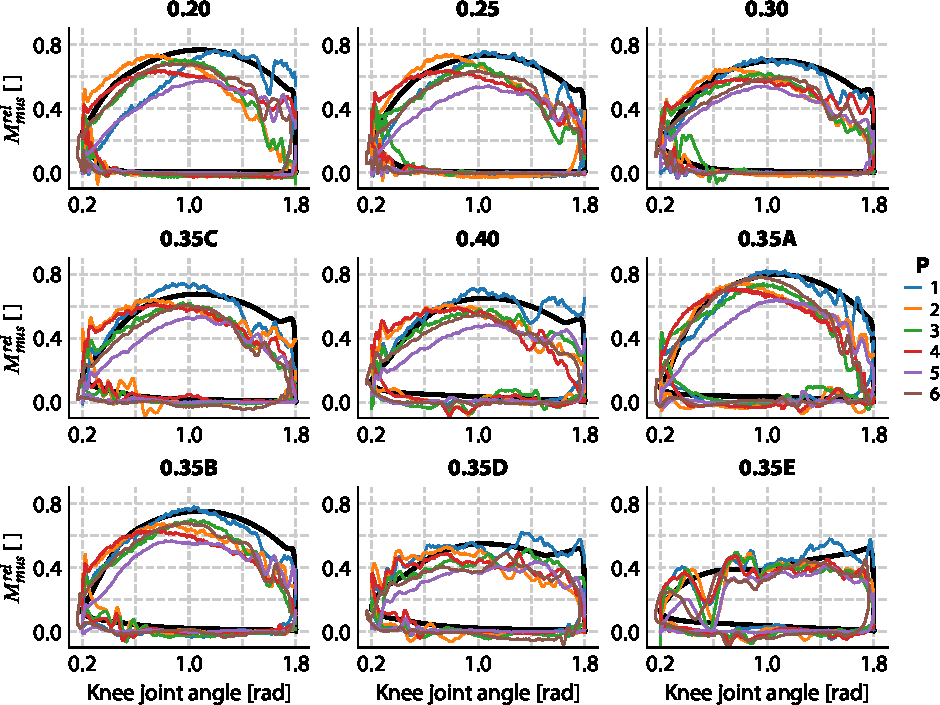
\includegraphics[keepaspectratio]{../figures/r_kinetics.pdf}}

}

\caption{\label{fig-r-kinetics}\textbf{Experimentally estimated and
model-predicted relative `muscular' knee joint moment
(\(M_{mus}^{rel}\)) for all conditions.} \(M_{mus}^{rel}\) was
calculated by dividing the `muscular' knee joint moment by the maximal
isometric knee joint moment of the individual participants (estimated
from the isometric knee joint moment-angle relationship; see
Figure~\ref{fig-r-te-isometric}) or by that of the model. The thick
black line depicts the predicted \(M_{mus}^{rel}\), while the thinner
coloured lines depicts \(M_{mus}^{rel}\) for each individual participant
(P). For each participant, \(M_{mus}^{rel}\) is shown for the cycle with
highest measured AMPO.}

\end{figure}%

\newpage{}

\begin{figure}[H]

\centering{

\pandocbounded{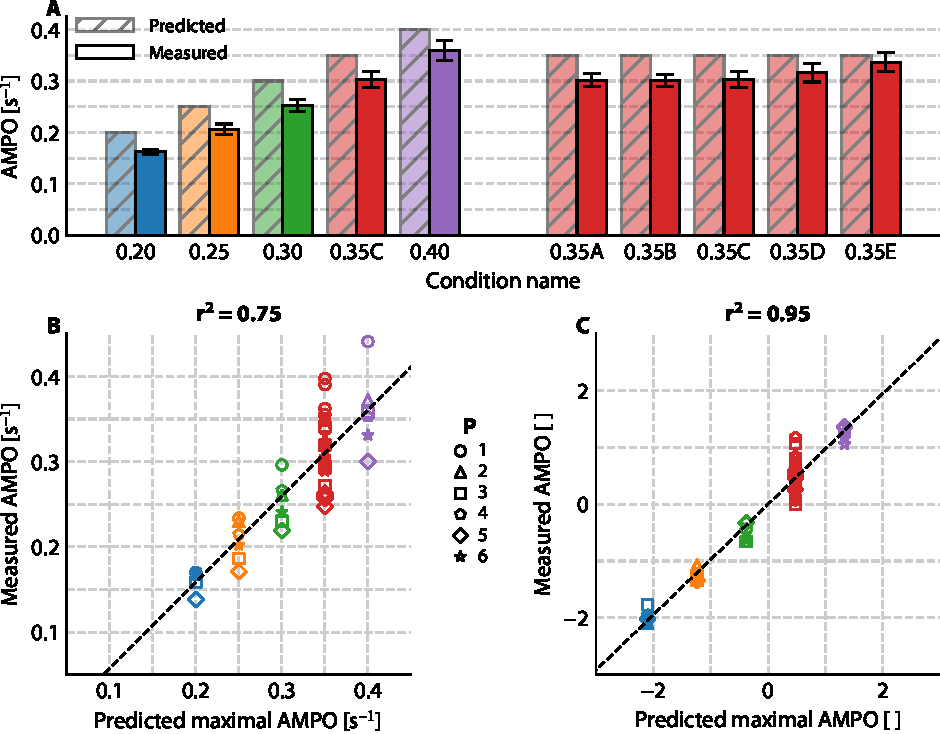
\includegraphics[keepaspectratio]{../figures/r_overview.pdf}}

}

\caption{\label{fig-r-overview}\textbf{Measured AMPO versus predicted
maximally attainable AMPO.} A) Barplot showing predicted values with
diagonal hatching and semi-transparent fill (\(\alpha\) = 0.5), and
experimentally measured values fully filled. Error bars denote the
standard error of the mean. B) Scatterplot of measured versus predicted
maximally attainable AMPO normalised by \(L_{CE}^{opt}\) and
\(F_{CE}^{max}\), with \(F_{CE}^{max}\) estimated individually for each
participant. C) Scatterplot of measured versus predicted maximally
attainable AMPO normalised to z-scores. Participants (P) are
distinguished by symbols.}

\end{figure}%

\newpage{}

\begin{table}[H]

\caption{\label{tbl-r-overview}Overview of experimental conditions and
measured AMPO per participant and condition.}

\centering{

 \begin{tabularx}{\textwidth}{|p{2.8cm}|*{9}{>{\centering\arraybackslash}X|}} \hline
  & \multicolumn{9}{|c|}{\itshape Condition} \\ \hline
  & \bfseries 0.20 & \bfseries 0.25 & \bfseries 0.30 & \bfseries 0.35C & \bfseries 0.40 & \bfseries 0.35A & \bfseries 0.35B & \bfseries 0.35D & \bfseries 0.35E \\ \hline
 \multicolumn{10}{|r|}{\itshape Movement characteristics} \\ \hline
 \bfseries CF [Hz]  & 0.44  & 0.59  & 0.75  & 0.93  & 1.13  & 0.79  & 0.83  & 1.13  & 1.35 \\ \hline 
 \bfseries FTS [ ]  & 0.35  & 0.40  & 0.45  & 0.51  & 0.58  & 0.72  & 0.61  & 0.46  & 0.48 \\ \hline 
 \bm{$T_{ext}$} \bfseries [s]  & 0.79  & 0.67  & 0.60  & 0.55  & 0.51  & 0.91  & 0.73  & 0.41  & 0.36 \\ \hline 
 \bm{$T_{flex}$} \bfseries [s]  & 1.46  & 1.02  & 0.73  & 0.53  & 0.38  & 0.36  & 0.48  & 0.48  & 0.38 \\ \hline 
 \multicolumn{10}{|r|}{\itshape AMPO} \\ \hline
 \bfseries Participant 1 [s\textsuperscript{-1}]  & 0.17  & 0.23  & 0.30  & 0.36  & 0.44  & 0.34  & 0.36  & 0.39  & 0.40 \\ \hline 
 \bfseries Participant 2 [s\textsuperscript{-1}]  & 0.17  & 0.23  & 0.26  & 0.32  & 0.37  & 0.32  & 0.30  & 0.32  & 0.35 \\ \hline 
 \bfseries Participant 3 [s\textsuperscript{-1}]  & 0.16  & 0.19  & 0.23  & 0.29  & 0.36  & 0.27  & 0.29  & 0.32  & 0.34 \\ \hline 
 \bfseries Participant 4 [s\textsuperscript{-1}]  & 0.17  & 0.21  & 0.27  & 0.30  & 0.35  & 0.30  & 0.29  & 0.30  & 0.35 \\ \hline 
 \bfseries Participant 5 [s\textsuperscript{-1}]  & 0.14  & 0.17  & 0.22  & 0.25  & 0.30  & 0.26  & 0.26  & 0.26  & 0.26 \\ \hline 
 \bfseries Participant 6 [s\textsuperscript{-1}]  & 0.17  & 0.20  & 0.24  & 0.29  & 0.33  & 0.31  & 0.30  & 0.30  & 0.32 \\ \hline 
 \bfseries Average $\pm$ SD [s\textsuperscript{-1}]  & 0.16 ± 0.01  & 0.21 ± 0.02  & 0.25 ± 0.03  & 0.30 ± 0.03  & 0.36 ± 0.04  & 0.30 ± 0.03  & 0.30 ± 0.03  & 0.32 ± 0.04  & 0.34 ± 0.04 \\ \hline 
 \bfseries Predicted [s\textsuperscript{-1}]  & 0.20  & 0.25  & 0.30  & 0.35  & 0.40  & 0.35  & 0.35  & 0.35  & 0.35 \\ \hline 
\end{tabularx}\break\hfill\footnotesize{CF denotes cycle frequency, FTS denotes fraction of cycle time spent shortening, $T_{ext}$ and $T_{flex}$ denote the knee joint extension and flexion time per cycle. Measured AMPO was normalised to the product of the participant's individually estimated $F_{CE}^{max}$ and the generic model parameter value of $L_{CE}^{opt}$, while predicted AMPO was normalised to the product of model parameters $F_{CE}^{max}$ and $L_{CE}^{opt}$ (see Methods). }

}

\end{table}%

\subsection{Influence of SSC parameters on the maximally attainable
AMPO}\label{influence-of-ssc-parameters-on-the-maximally-attainable-ampo}

\begin{Shaded}
\begin{Highlighting}[]
\CommentTok{\# \%\% [markdown]}
\CommentTok{\# {-}{-}{-}}
\CommentTok{\# title: Influence SSC parameters}
\CommentTok{\# {-}{-}{-}}

\CommentTok{\# \%\% [markdown]}
\CommentTok{"""}
\CommentTok{This script computes the results of the section \textquotesingle{}Influence of SSC parameters }
\CommentTok{on the maximally attainable AMPO\textquotesingle{}. }

\CommentTok{Specifically, it performs the following steps:}
\CommentTok{    }
\CommentTok{{-}   Loads muscle parameters from a pickle file (\textasciigrave{}VAS\_muspar.pkl\textasciigrave{}).}
\CommentTok{{-}   Defines parameter grids for SSC parameters: }
\CommentTok{    {-}   CF (cycle frequency)}
\CommentTok{    {-}   FTS (fraction of the cycle time spent shortening)}
\CommentTok{    {-}   KJE (knee joint excursion)}
\CommentTok{{-}   Loads precomputed simulation data for each combination of SSC parameters.}
\CommentTok{{-}   Computes the AMPO (average mechanical power output) normalised by }
\CommentTok{    maximal isometric CE force (fmax) and optimal CE length (lceopt).}
\CommentTok{{-}   Interpolates the AMPO values onto a finer 3D grid for smoother analysis.}
\CommentTok{{-}   Determines the maximum AMPO and the corresponding optimal SSC parameters.}

\CommentTok{"""}

\CommentTok{\# \%\% [markdown]}
\CommentTok{"""}
\CommentTok{\#\# Load packages \& set directories}
\CommentTok{"""}

\CommentTok{\#\%\% Imports etc.}
\ImportTok{import}\NormalTok{ os, sys, pickle}
\ImportTok{import}\NormalTok{ numpy }\ImportTok{as}\NormalTok{ np}
\ImportTok{import}\NormalTok{ pandas }\ImportTok{as}\NormalTok{ pd}
\ImportTok{from}\NormalTok{ scipy }\ImportTok{import}\NormalTok{ integrate, interpolate}
\ImportTok{from}\NormalTok{ pathlib }\ImportTok{import}\NormalTok{ Path}

\CommentTok{\# Paths}
\NormalTok{cwd }\OperatorTok{=}\NormalTok{ Path.cwd()}
\NormalTok{baseDir }\OperatorTok{=}\NormalTok{ cwd.parent}
\NormalTok{dataDir }\OperatorTok{=}\NormalTok{ baseDir }\OperatorTok{/} \StringTok{\textquotesingle{}data\textquotesingle{}}
\NormalTok{funcDir }\OperatorTok{=}\NormalTok{ baseDir }\OperatorTok{/} \StringTok{\textquotesingle{}analysis\textquotesingle{}} \OperatorTok{/} \StringTok{\textquotesingle{}functions\textquotesingle{}}
\NormalTok{sys.path.append(}\BuiltInTok{str}\NormalTok{(funcDir))}

\CommentTok{\# \%\% [markdown]}
\CommentTok{"""}
\CommentTok{\#\# Extract AMPO of each condition}
\CommentTok{"""}

\CommentTok{\#\%\% Extract AMPO of each condition}
\CommentTok{\# Load Parameters}
\NormalTok{parFile }\OperatorTok{=}\NormalTok{ os.path.join(dataDir, }\StringTok{\textquotesingle{}VAS\_muspar.pkl\textquotesingle{}}\NormalTok{)}
\NormalTok{muspar }\OperatorTok{=}\NormalTok{ pickle.load(}\BuiltInTok{open}\NormalTok{(parFile, }\StringTok{\textquotesingle{}rb\textquotesingle{}}\NormalTok{))}

\CommentTok{\# Define parameter grids}
\NormalTok{kjeSet }\OperatorTok{=}\NormalTok{ np.arange(}\FloatTok{0.8}\NormalTok{, }\FloatTok{2.01}\NormalTok{, }\FloatTok{0.1}\NormalTok{)}
\NormalTok{cfSet }\OperatorTok{=}\NormalTok{ np.arange(}\FloatTok{0.4}\NormalTok{, }\FloatTok{3.1}\NormalTok{, }\FloatTok{0.2}\NormalTok{)}
\NormalTok{ftsSet }\OperatorTok{=}\NormalTok{ np.arange(}\FloatTok{0.05}\NormalTok{, }\FloatTok{0.96}\NormalTok{, }\FloatTok{0.05}\NormalTok{)}

\CommentTok{\# Initialize AMPO array}
\NormalTok{AMPO }\OperatorTok{=}\NormalTok{ np.full((}\BuiltInTok{len}\NormalTok{(kjeSet), }\BuiltInTok{len}\NormalTok{(ftsSet), }\BuiltInTok{len}\NormalTok{(cfSet)), np.nan)}

\CommentTok{\# Load simulation data and compute AMPO}
\ControlFlowTok{for}\NormalTok{ iKJE, kje }\KeywordTok{in} \BuiltInTok{enumerate}\NormalTok{(kjeSet):}
    \ControlFlowTok{for}\NormalTok{ iFTS, fts }\KeywordTok{in} \BuiltInTok{enumerate}\NormalTok{(ftsSet):}
        \ControlFlowTok{for}\NormalTok{ iCF, cf }\KeywordTok{in} \BuiltInTok{enumerate}\NormalTok{(cfSet):}
\NormalTok{            filepath }\OperatorTok{=}\NormalTok{ os.path.join(dataDir, }\StringTok{\textquotesingle{}simsSSC\textquotesingle{}}\NormalTok{,}
                                    \SpecialStringTok{f\textquotesingle{}cf}\SpecialCharTok{\{}\NormalTok{cf}\SpecialCharTok{:0.2f\}}\SpecialStringTok{Hz\_fts}\SpecialCharTok{\{}\NormalTok{fts}\SpecialCharTok{:0.2f\}}\SpecialStringTok{\_kje}\SpecialCharTok{\{}\NormalTok{kje}\SpecialCharTok{:0.2f\}}\SpecialStringTok{rad.csv\textquotesingle{}}\NormalTok{)}
            \ControlFlowTok{try}\NormalTok{:}
\NormalTok{                df }\OperatorTok{=}\NormalTok{ pd.read\_csv(filepath)}
\NormalTok{                data }\OperatorTok{=}\NormalTok{ df.T.to\_numpy()}
\NormalTok{                time, phi, stim, fsee, gamma, lcerel, q, lmtc, fisomrel }\OperatorTok{=}\NormalTok{ data}
                \CommentTok{\# Compute AMPO normalized by fmax and lce\_opt}
\NormalTok{                AMPO[iKJE, iFTS, iCF] }\OperatorTok{=} \OperatorTok{{-}}\NormalTok{integrate.trapezoid(fsee }\OperatorTok{*}\NormalTok{ muspar[}\StringTok{\textquotesingle{}A1\textquotesingle{}}\NormalTok{], phi) }\OperatorTok{*}\NormalTok{ cf }\OperatorTok{/}\NormalTok{ (muspar[}\StringTok{\textquotesingle{}fmax\textquotesingle{}}\NormalTok{] }\OperatorTok{*}\NormalTok{ muspar[}\StringTok{\textquotesingle{}lce\_opt\textquotesingle{}}\NormalTok{])}
            \ControlFlowTok{except} \PreprocessorTok{Exception}\NormalTok{:}
\NormalTok{                AMPO[iKJE, iFTS, iCF] }\OperatorTok{=}\NormalTok{ np.nan}

\CommentTok{\# Create meshgrid for axes (match AMPO shape)}
\NormalTok{Z, Y, X }\OperatorTok{=}\NormalTok{ np.meshgrid(kjeSet, ftsSet, cfSet, indexing}\OperatorTok{=}\StringTok{\textquotesingle{}ij\textquotesingle{}}\NormalTok{)  }\CommentTok{\# ij indexing: Z=kje, Y=fts, X=cf}

\CommentTok{\# Flatten data for interpolation}
\NormalTok{x\_flat }\OperatorTok{=}\NormalTok{ X.flatten()}
\NormalTok{y\_flat }\OperatorTok{=}\NormalTok{ Y.flatten()}
\NormalTok{z\_flat }\OperatorTok{=}\NormalTok{ Z.flatten()}
\NormalTok{data\_flat }\OperatorTok{=}\NormalTok{ AMPO.flatten()}

\CommentTok{\# Define finer interpolation grid}
\NormalTok{kje\_fine }\OperatorTok{=}\NormalTok{ np.linspace(kjeSet[}\DecValTok{0}\NormalTok{], kjeSet[}\OperatorTok{{-}}\DecValTok{1}\NormalTok{], }\DecValTok{100}\NormalTok{)}
\NormalTok{fts\_fine }\OperatorTok{=}\NormalTok{ np.linspace(ftsSet[}\DecValTok{0}\NormalTok{], ftsSet[}\OperatorTok{{-}}\DecValTok{1}\NormalTok{], }\DecValTok{100}\NormalTok{)}
\NormalTok{cf\_fine  }\OperatorTok{=}\NormalTok{ np.linspace(cfSet[}\DecValTok{0}\NormalTok{], cfSet[}\OperatorTok{{-}}\DecValTok{1}\NormalTok{], }\DecValTok{100}\NormalTok{)}

\NormalTok{Zf, Yf, Xf }\OperatorTok{=}\NormalTok{ np.meshgrid(kje\_fine, fts\_fine, cf\_fine, indexing}\OperatorTok{=}\StringTok{\textquotesingle{}ij\textquotesingle{}}\NormalTok{)}

\CommentTok{\# Interpolate}
\NormalTok{AMPO\_fine }\OperatorTok{=}\NormalTok{ interpolate.griddata((z\_flat, y\_flat, x\_flat), data\_flat, (Zf, Yf, Xf), method}\OperatorTok{=}\StringTok{\textquotesingle{}linear\textquotesingle{}}\NormalTok{)}

\CommentTok{\# Find maximum AMPO and corresponding parameters}
\NormalTok{max\_idx }\OperatorTok{=}\NormalTok{ np.nanargmax(AMPO\_fine)}
\NormalTok{iKJE, iFTS, iCF }\OperatorTok{=}\NormalTok{ np.unravel\_index(max\_idx, AMPO\_fine.shape)}

\NormalTok{opt\_kje  }\OperatorTok{=} \SpecialStringTok{f"}\SpecialCharTok{\{}\NormalTok{Zf[iKJE, iFTS, iCF]}\SpecialCharTok{:0.1f\}}\SpecialStringTok{"}
\NormalTok{opt\_fts  }\OperatorTok{=} \SpecialStringTok{f"}\SpecialCharTok{\{}\NormalTok{Yf[iKJE, iFTS, iCF]}\SpecialCharTok{:0.2f\}}\SpecialStringTok{"}
\NormalTok{opt\_cf   }\OperatorTok{=} \SpecialStringTok{f"}\SpecialCharTok{\{}\NormalTok{Xf[iKJE, iFTS, iCF]}\SpecialCharTok{:0.1f\}}\SpecialStringTok{"}
\NormalTok{maxAMPO }\OperatorTok{=}\NormalTok{ AMPO\_fine[iKJE, iFTS, iCF]}

\CommentTok{\# Print results}
\BuiltInTok{print}\NormalTok{(}\SpecialStringTok{f"Maximum AMPO: }\SpecialCharTok{\{}\NormalTok{maxAMPO}\SpecialCharTok{:0.3f\}}\SpecialStringTok{"}\NormalTok{)}
\BuiltInTok{print}\NormalTok{(}\SpecialStringTok{f"Optimal KJE: }\SpecialCharTok{\{}\NormalTok{opt\_kje}\SpecialCharTok{\}}\SpecialStringTok{ rad, FTS: }\SpecialCharTok{\{}\NormalTok{opt\_fts}\SpecialCharTok{\}}\SpecialStringTok{, CF: }\SpecialCharTok{\{}\NormalTok{opt\_cf}\SpecialCharTok{\}}\SpecialStringTok{ Hz"}\NormalTok{)}
\end{Highlighting}
\end{Shaded}

Having established that the influence of SSC parameters - cycle
frequency, FTS and knee joint excursion - on the maximally attainable
AMPO was accurately predicted by our Hill-type MTC model, we now examine
the effects of the SSC parameters in detail. The predicted effect of
cycle frequency and FTS at four distinct knee joint excursions are
depicted in Figure~\ref{fig-r-contour}. The optimal combination of SSC
parameters was predicted to be a cycle frequency of about 1.6 Hz, a FTS
of about 0.80 and a knee joint excursion of about 2.0 rad. Because knee
joint movements were centred around 1.0 rad, knee joint excursions
beyond 2.0 rad would result in knee hyperextension and were therefore
not physiologically meaningful. Nevertheless, model predictions showed
that knee joint excursions above 2.0 rad did not further increase the
maximally attainable AMPO.

Regarding the interrelationship between the SSC parameters, we found
that the optimal FTS for AMPO remained relatively stable across the
range of cycle frequencies and knee joint excursions studied,
consistently ranging between 0.78 and 0.85. The largest variation in
optimal FTS was observed at the smallest knee joint excursion studied
(0.8 rad). By contrast, optimal cycle frequency showed substantial
sensitivity to changes in FTS. Additionally, a strong interaction was
found between cycle frequency and knee joint excursion: increasing one
necessitates a decrease in the other to maximise AMPO.

\begin{figure}[H]

\centering{

\pandocbounded{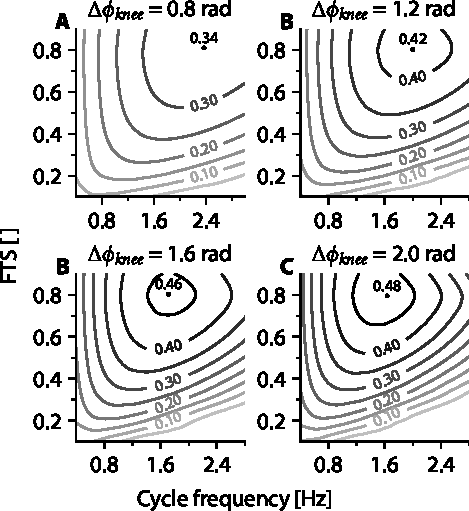
\includegraphics[keepaspectratio]{../figures/r_contours.pdf}}

}

\caption{\label{fig-r-contour}\textbf{Predicted maximally attainable
AMPO as a function of SSC parameters: cycle frequency, fraction of cycle
time spent shortening (FTS), and knee joint excursion
(\(\Delta \phi_{\text{knee}}\)).} For each subplot, one SSC parameter
was fixed, while the influence of the other two parameters on maximally
attainable AMPO (normalised to \(L_{CE}^{opt}\) and \(F_{CE}^{max}\)) is
depicted as contour lines. Dots indicate peak AMPO, corresponding to the
optimal combination of the two varying SSC parameters; values are shown
at the top left of each dot. A--D) Predicted maximally attainable AMPO
as a function of cycle frequency and FTS for four distinct knee joint
excursions. E--H) Predicted maximally attainable AMPO as a function of
cycle frequency and knee joint excursion for four distinct FTS values.}

\end{figure}%

\section{Discussion}\label{discussion}

In this study, we examined the influence of imposed knee joint movement
on the maximally attainable AMPO of human \emph{m. quadriceps femoris}
by combining experiments with simulations and optimisations using a
Hill-type MTC model. Our findings revealed a strong correlation between
measured AMPO and predicted maximally attainable AMPO, for a wide
variety of imposed knee joint movements. Model predictions revealed that
the maximally attainable AMPO peaks at a cycle frequency of about 1.6
Hz, an FTS of about 0.80, and a knee joint excursion of about 2.0 rad.
While the optimal knee joint excursion was predicted to decrease with
increasing cycle frequency and vice versa, the optimal FTS was predicted
to be largely unaffected by changes in cycle frequency and knee joint
excursion.

\subsection{Evaluation of model predictions against experimental
data}\label{evaluation-of-model-predictions-against-experimental-data}

Measured AMPO and predicted maximally attainable AMPO were strongly
correlated, with measured AMPO being 87 ± 10\% of the predicted values
on average. The lower measured AMPO primarily resulted from \(M_{mus}\)
values that were lower than values predicted for knee extension. It
should be noted that, in theory, predicted maximally attainable AMPO
should always exceed measured AMPO. For the model predictions, \emph{m.
quadriceps femoris} activation was set to be optimal in both timing and
magnitude, and no hamstring co-contraction occurs. By contrast,
participant muscle activation is inherently suboptimal.

Regarding \emph{m. quadriceps femoris} activation, EMG of \emph{m.
quadriceps femoris} rose just at the transition from flexion to
extension, causing \(M_{mus}\) to increase at this time instant. Thus,
we consider the timing of \emph{m. quadriceps femoris} of participants
to be adequate. However, EMG of \emph{m. quadriceps femoris} did not
exceed 100\% of \(EMG^{MVC}\) for all conditions amongst five of the six
participants. This differs from previous studies (e.g.
\citeproc{ref-bobbert_evaluation_1993}{Bobbert and Harlaar, 1993};
\citeproc{ref-kellis_muscle_1998}{Kellis and Baltzopoulos, 1998};
\citeproc{ref-westing_muscle_1991}{Westing et al., 1991}), which
reported \emph{m. quadriceps femoris} EMG values slightly exceeding
100\% in knee dynamometer experiments. Hence, submaximal \emph{m.
quadriceps femoris} activation may partly explain the lower \(M_{mus}\)
relative to predicted values.

Regarding the co-contraction of the hamstring muscle group, EMG of the
hamstring muscle group during knee extension was 17.3 ± 12.4\% of
\(EMG^{MVC}\), consistent with previous studies (e.g.
\citeproc{ref-kellis_muscle_1998}{Kellis and Baltzopoulos, 1998};
\citeproc{ref-snow_antagonist_1993}{Snow et al., 1993}). When
interpreting surface EMG as a proxy for muscle activation, potential
crosstalk should be considered. In the context of this study, it is
possible that both quadriceps and hamstrings activation are slightly
overestimated due to crosstalk. However, the effect of EMG crosstalk on
the net knee joint moment is probably smaller than suggested by EMG
values alone, since the maximal isometric force of the hamstring muscle
group is approximately 2.5 times lower than that of \emph{m. quadriceps
femoris} (e.g. \citeproc{ref-prietto_vivo_1989}{Prietto and Caiozzo,
1989}). Nevertheless, it is clear that co-contraction of hamstrings
during knee extension may also partly explain the slight deficit in
\(M_{mus}\) relative to predicted values.

Measured and predicted \(M_{mus}\) were normalised to the maximal
isometric force (\(F_{CE}^{max}\); see Figure~\ref{fig-r-kinetics}).
\(F_{CE}^{max}\) was estimated individually for each participant from
their measured isometric knee joint angle-moment relationship. In most
cases, the actual participant's maximum measured isometric knee joint
moment was higher than the maximal value of the model (see
Figure~\ref{fig-r-te-isometric}), indicating that \(F_{CE}^{max}\) was
not overestimated. Nevertheless, it should be noted that any inaccuracy
in \(F_{CE}^{max}\) directly affects normalised \(M_{mus}\). Aside from
a simple normalisation of AMPO with \(F_{CE}^{max}\), predictions were
not individually tailored. Consequently, properties of participants'
\emph{m. quadriceps femoris} could be different from the properties used
in the Hill-type MTC model. Measured force rise was generally slower
than predicted (see Figure~\ref{fig-r-kinetics}), suggesting that the
model's activation dynamics may have been slightly too fast. Moreover,
measured \(M_{mus}\) was consistently lower across various knee joint
angles, even where maximal activation was achieved in both experiment
and model. The force--length relationship likely played only a minor
role, because the isometric knee joint moment--angle relationship was
reasonably similar for participants and the model. Instead, the
force--velocity relationship appears to be the main contributor. In our
model, the decline in knee extension moment with increasing angular
velocity was at the lower end of experimentally observed values (for
review, see \citeproc{ref-chen_joint_2025}{Chen and Franklin, 2025}).
Overall, the slight deficit in \(M_{mus}\) relative to predicted values
may partly be explained by differences between the generic model
properties and participants' \emph{m. quadriceps femoris} properties.
Obviously, all other muscle properties implemented in the model may not
exactly match those of (or between) participants' \emph{m. quadriceps
femoris}. For example, the moment arm (assumed to be constant in our
model) directly influences \(M_{mus}\), yet it was also used to estimate
\(F_{CE}^{max}\); thus, any over- or underestimation would be
compensated during normalisation. Additionally, the moment arm
determines MTC velocity during knee extension, thereby affecting
\(M_{mus}\) mainly through its influence on CE shortening velocity.
Lastly, SEE compliance influences CE dynamics; the additional dynamics
resulting from this CE-SEE interaction is captured in our model. Under
the present experimental conditions, discrepancies between CE and SEE
length and velocity are predicted to be small, as MTC excursions
(\textasciitilde6.7 cm) were substantially larger than SEE excursions
(\textasciitilde0.6 cm). This suggests that CE--SEE interaction, and
therefore any mismatch between modelled and participant-specific SEE
compliance, had only a minor influence on \(M_{mus}\). We expect that,
with individually tailored models, differences between experimental and
predicted \(M_{mus}\) would have been even smaller than differences
reported in this study.

We emphasise that our aim was not to precisely predict the magnitude of
\(M_{mus}\) over time, but rather to examine the influence of SSC
parameters on the maximally attainable AMPO. Thus, it is promising that
we predict the magnitude of the maximally attainable AMPO remarkably
well using a relatively simple Hill-type MTC model with generic
parameter values obtained from literature, despite the aforementioned
methodological limitations. Moreover, when assessing the influence of
SSC parameters on the maximally attainable AMPO, the relative change in
AMPO is more informative than its (average) magnitude. In this context,
it is particularly encouraging that AMPO normalised to z-scores revealed
a very strong correlation between predictions and measurements
(r\textsuperscript{2} = 0.95). This finding aligns with previous studies
demonstrating that Hill-type MTC models reliably predict mechanical
behaviour, especially during concentric contractions (e.g.
\citeproc{ref-van_ingen_schenau_simulation_1988}{Ingen Schenau et al.,
1988}; \citeproc{ref-lemaire_comparison_2016}{Lemaire et al., 2016};
\citeproc{ref-sandercock_force_1997}{Sandercock and Heckman, 1997};
\citeproc{ref-wakeling_predicting_1999}{Wakeling and Johnston, 1999};
\citeproc{ref-van_zandwijk_twitch_1996}{Zandwijk et al., 1996}).
Concentric contractions primarily determine maximally attainable AMPO.
All in all, we attribute the small discrepancy between measured and
predicted maximally attainable AMPO to (a combination of) several
factors, such as suboptimal \emph{m. quadriceps femoris} activation,
hamstring co-contraction, and generic model assumptions. Nevertheless,
predictions aligned remarkably well with measurements, demonstrating the
validity of the predicted influence of SSC parameters on the maximally
attainable AMPO of human \emph{m. quadriceps femoris}.

\subsection{Results agree well with available
literature}\label{results-agree-well-with-available-literature}

In the first part of the current study, \(L_{SEE}^0\), \(L_{CE}^{opt}\)
and \(F_{CE}^{max}\) were estimated for each participant individually
based on isometric measurements at nine different knee joint angles. The
measured net knee joint moment-angle relationship of participants was in
line with literature (e.g. \citeproc{ref-anderson_maximum_2007}{Anderson
et al., 2007}; \citeproc{ref-van_eijden_forces_2008}{Eijden et al.,
2008}; \citeproc{ref-murray_strength_1980}{Murray et al., 1980}). The
estimation of the muscle model parameters was deemed successful as the
root mean square error between the measured isometric knee joint moment
and the musculoskeletal predicted isometric knee joint moment was low
(6.6 ± 2.2\% of \(F_{CE}^{max}\) on average). Additionally, values of
\(L_{SEE}^0\) and \(L_{CE}^{opt}\) corresponded well with values
obtained from cadavers (e.g.
\citeproc{ref-friederich_muscle_1990}{Friederich and Brand, 1990};
\citeproc{ref-ward_are_2009}{Ward et al., 2009};
\citeproc{ref-wickiewicz_muscle_1983}{Wickiewicz et al., 1983}) and
values used in other modelling studies (e.g.
\citeproc{ref-anderson_dynamic_1999}{Anderson and Pandy, 1999};
\citeproc{ref-van_soest_contribution_1993}{Soest and Bobbert, 1993}).
Overall, we conclude that the values of \(L_{SEE}^0\), \(L_{CE}^{opt}\)
and \(F_{CE}^{max}\) were successfully estimated.

In the second part of the current study, we examined the maximally
attainable AMPO for a large set of imposed knee joint movements. As our
study is the first to investigate this for human muscle, the only
available data for comparison are those of \emph{in vitro} or \emph{in
situ} studies on animal muscle. Whereas we influenced muscle length
indirectly by imposing knee joint excursions, those studies directly
imposed muscle length excursions. Those studies on animal muscle show
that an increase in cycle frequency leads to a decrease in the
AMPO-optimal length excursion, muscle stimulation duration and
mechanical work per cycle (e.g. \citeproc{ref-askew_effects_1997}{Askew
and Marsh, 1997}; \citeproc{ref-james_mechanical_1995}{James et al.,
1995}; \citeproc{ref-josephson_mechanical_1985}{Josephson, 1985};
\citeproc{ref-reuvers_maximising_2025}{Reuvers et al., 2025}). Our
findings for human \emph{m. quadriceps femoris} align with these
observations. Additionally, in accordance with Askew and Marsh
(\citeproc{ref-askew_effects_1997}{1997}) and Reuvers et al.
(\citeproc{ref-reuvers_maximising_2025}{2025}), we found that the
optimal (length) excursion increases with increasing FTS and decreasing
cycle frequency.

Regarding the values of cycle frequency, FTS and muscle fibre length
excursion per se, it should be noted that these values substantially
differ due to differences in muscle properties (e.g.~maximal shortening
velocity, excitation dynamics etc.). Accordingly, the optimal cycle
frequency of about 1.6 Hz observed for human \emph{m. quadriceps
femoris} contrasts with about 4 Hz for mouse \emph{m. soleus}
(\citeproc{ref-askew_effects_1997}{Askew and Marsh, 1997}), about 9 Hz
for mouse \emph{m. extensor digitorum longus}
(\citeproc{ref-askew_effects_1997}{Askew and Marsh, 1997}), and about
3.5 Hz for rat \emph{m. gastrocnemius medialis}
(\citeproc{ref-reuvers_maximising_2025}{Reuvers et al., 2025}).
Similarly, optimal muscle fibre length excursion, expressed as a
percentage of the optimum fibre length, varies across muscles: 22\% for
mouse \emph{m. soleus} (\citeproc{ref-askew_effects_1997}{Askew and
Marsh, 1997}), 16\% for mouse \emph{m. extensor digitorum longus}
(\citeproc{ref-askew_effects_1997}{Askew and Marsh, 1997}), and 58\% for
rat \emph{m. gastrocnemius medialis}
(\citeproc{ref-reuvers_maximising_2025}{Reuvers et al., 2025}). All of
these values are considerably lower than the 85\% reported here for
human \emph{m. quadriceps femoris}. Interestingly, the optimal FTS of
0.80 for human \emph{m. quadriceps femoris} is comparable to the range
of 0.80-0.90 observed in animal muscle
(\citeproc{ref-askew_effects_1997}{Askew and Marsh, 1997};
\citeproc{ref-reuvers_maximising_2025}{Reuvers et al., 2025}). The
optimal FTS is predominantly a trade-off between (the negative effect
of) the force-velocity relationship on the one hand and (the negative
effect of) the excitation dynamics on the other hand (for details, see
\citeproc{ref-reuvers_maximising_2025}{Reuvers et al., 2025}). Both
factors depend on muscle fibre type; their negative effect on AMPO
increases with slower muscle fibre types. Consequently, the optimal FTS
is expected to be relatively robust for variations in muscle fibre type.
Therefore, it is promising that the optimal FTS in our study aligns with
those observed in animal muscle. Overall, our findings are consistent
with the available literature, which strengthens our confidence in the
validity of the results.

\subsection{Experimental constraints and physiological
relevance}\label{experimental-constraints-and-physiological-relevance}

In extensive pilot experiments, we explored a range of knee joint
movements with different angular velocities and accelerations. Based on
these pilot experiments and safety considerations, we limited knee joint
acceleration to 50 rad/s\textsuperscript{2}, thereby also limiting the
(maximum achievable) knee joint angular velocity. As a result, only a
subset of combinations of SSC parameters --- cycle frequency, FTS, and
knee joint excursion --- could be tested experimentally. Importantly,
this does not imply that higher velocities or accelerations are
physiologically infeasible for human knee joint movements. In fact,
substantially higher values are reached during various motor activities
(for review, see \citeproc{ref-grimmer_human_2020}{Grimmer et al.,
2020}). For example, during sprint cycling, knee joint angular
velocities reach 5--10 rad/s, and angular accelerations exceed 100
rad/s\textsuperscript{2}. During sprint running these values are even
higher, with knee joint angular velocities reaching about 20 rad/s and
angular accelerations up to 200 rad/s\textsuperscript{2}. Therefore, the
joint movements that were not feasible in our experiment are nonetheless
physiologically meaningful.

\subsection{Physiological implications for human
movement}\label{physiological-implications-for-human-movement}

AMPO in our study was normalised to the product of \(F_{CE}^{max}\) and
\(L_{CE}^{opt}\). This allowed comparison across participants, but also
allows us to extend our findings to muscles of similar fibre types. For
typical values of \(L_{CE}^{opt}\)=9.3 cm and \(F_{CE}^{max}\)=5250 N
for \emph{mm. vastii}, and \(L_{CE}^{opt}\)=8.1 cm and
\(F_{CE}^{max}\)=1750 N for \emph{m. rectus femoris}
(\citeproc{ref-van_soest_which_2000}{Soest and Casius, 2000}), peak AMPO
for \emph{m. quadriceps femoris} is predicted to be approximately 300 W
per leg at the optimal combination of SSC parameters. This value may be
used as a benchmark in assessing maximum AMPO of human \emph{m.
quadriceps femoris} AMPO in any short-duration task that involves
periodic motion.

In our study, we measured AMPO of the human \emph{m. quadriceps femoris}
during fully imposed knee joint movements. This setup allowed us to
directly control the kinematics of the stretch-shortening cycle (SSC)
and to ensure that knee joint movements were identical across
participants. We show that SSC parameters substantially influence
maximally attainable AMPO (see Figure~\ref{fig-r-contour}). For example,
increasing FTS from 0.5 to its optimal value of about 0.8 is predicted
to improve AMPO by about 25\% at the optimal cycle frequency, with
smaller effects at lower frequencies and larger effects at higher
frequencies. The resulting insights into the influence of SSC parameters
on maximally attainable AMPO can be used to analyse any SSC of any
muscle or muscle group, irrespective of whether this SSC arises from
fully imposed movements or from unconstrained/self-generated movements.
For any SSC, we can now readily estimate the maximal AMPO at the
observed kinematics for any muscle (group), and relate that to the
maximally attainable AMPO of that muscle (group).

In most real-world situations, movements are not fully constrained and
typically involve several mechanical and kinematic degrees of freedom.
In such cases, movements arise from muscle forces and mechanical
interactions with the environment, which in turn determine the SSCs of
the muscles involved. This means that, for example, during an all-out
sprint cycling task, the coordination problem is to find muscle
activations such that the total AMPO of all muscles combined is
maximised over a full cycle. This inevitably leads to a trade-off
between the contributions of individual muscles to the total AMPO. Our
results provide not only insight into the mechanics of such a trade-off,
but may also help in designing equipment that interacts with the
musculoskeletal system to improve AMPO. For example, our results
indicate that muscles with a larger volume should spend more time
shortening than lengthening compared to muscles with a smaller volume in
order to maximise the total AMPO. In many periodic sports, however, the
shortening duration of \emph{m. quadriceps femoris} does not exceed the
lengthening duration. For instance, FTS ranges from 0.3--0.5 in rowing
(\citeproc{ref-bechard_total_2009}{Bechard et al., 2009};
\citeproc{ref-ettema_role_2022}{Ettema et al., 2022}), is approximately
0.3 in cross-country skiing
(\citeproc{ref-nilsson_crosscountry_2004}{Nilsson et al., 2004};
\citeproc{ref-pellegrini_gait_2014}{Pellegrini et al., 2014}), and is
around 0.5 in cycling (\citeproc{ref-bobbert_effect_2020}{Bobbert et
al., 2020}). Interestingly, in a clever experiment, Martin et al.
(\citeproc{ref-martin_pedal_2002}{2002}) showed that during single-leg
cycling, the maximal AMPO can be improved by about 4\% when the
downstroke duration is approximately 10\% longer than the upstroke
duration. This longer downstroke duration allows the large leg muscles
to spend more time shortening than lengthening, leading to an increase
in their AMPO that more than offsets the decrease in AMPO of other
(smaller) muscles that unavoidably spend less time shortening than
lengthening. This example highlight that redesign of equipment that
allows muscles to operate closer to their optimal SSC parameters, has
the potential to result in improved performance.

\subsection{Conclusion}\label{conclusion}

In this study, we examined how SSC parameters --- cycle frequency, FTS,
and knee joint excursion --- influence the maximally attainable AMPO of
human \emph{m. quadriceps femoris} during short-duration, all-out
(sprint) conditions. Because only a subset of SSC parameters can be
tested experimentally, we combined experiments with musculoskeletal
modelling. Differences in maximally attainable AMPO were adequately
predicted by our Hill-type MTC model, justifying its use to examine the
effect of SSC parameters on maximally attainable AMPO in detail. Model
predictions showed a substantial influence of SSC parameters on the
maximally attainable AMPO. Specifically, predictions revealed a strong
interaction between cycle frequency and knee joint excursion: increasing
one necessitates a decrease in the other to maximise AMPO. Even more
interestingly, in order to maximise AMPO, \emph{m. quadriceps femoris}
should spend about 80\% of the cycle duration while shortening,
independent of cycle frequency and/or knee joint excursion.

\newpage{}

\appendix
\phantomsection

\section*{Appendix}\label{appendix}
\addcontentsline{toc}{section}{Appendix}

\setcounter{subsection}{0} % Reset subsection counter

% Define subsection numbering in appendix as S1, S2, ...
\renewcommand{\thesubsection}{A\arabic{subsection}}

\renewcommand{\thetable}{A\arabic{table}}
\setcounter{table}{0}

\subsection{Selection of experimental conditions}\label{sec-s-expcond}

With our musculoskeletal model we predicted the maximally attainable
AMPO for knee joint movements with different constant knee angular
velocities during flexion and extension. Thus, the knee joint angular
velocity changed instantaneously at the switch from flexion to extension
(and vice versa), and the knee joint angular acceleration at that
instant was infinitely high/low. Clearly, infinite knee joint
accelerations cannot be achieved in an experimental setup. Instead, we
chose to impose a constant knee angular acceleration until a predefined
knee joint angular velocity was achieved --- determined by the
combination of cycle frequency, FTS, knee joint angle excursion and
constant knee angular acceleration --- in order to achieve the highest
cycle frequency and the greatest difference between maximal and minimal
FTS. In extensive pilot tests, we determined that 50
rad/s\textsuperscript{2} was the highest knee angular acceleration that
participants were comfortable with and was used as an upper limit for
the experiment. Accordingly, the experimental conditions were selected
from the knee joint movement that were experimentally feasible (see
Figure~\ref{fig-m-conditions}).

Due to the limit on maximal knee joint acceleration, the imposed knee
joint movement in the experiment were slightly different from those with
a constant knee angular velocity (i.e.~with no limit on knee angular
acceleration; see \quartoappfigref{appfig-dino-vs-cv}). As a result, the
maximally attainable AMPO differed slightly between those two for the
same set of SSC parameters. Therefore, we derived predictions of the
maximally attainable AMPO for knee joint movement with a limit of 50
rad/\textsuperscript{s}2 on the knee angular acceleration (see
Figure~\ref{fig-m-conditions}).

\begin{appfig}

\centering{

\pandocbounded{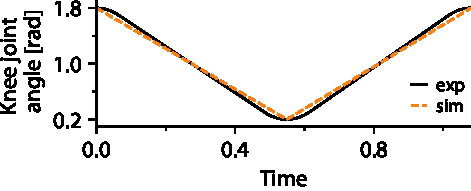
\includegraphics[keepaspectratio]{../figures/s_dino_vs_cv.pdf}}

}

\caption{\label{appfig-dino-vs-cv}\textbf{Comparison between knee joint
movements during the experiment and simulations.} In the experiment,
knee joint movements were limited to an angular acceleration of 50
rad/s\textsuperscript{2}. In contrast, in the simulations, knee joint
movements were used with different constant angular velocities for
flexion and extension in order to simulate a broad range knee joint
movements.}

\end{appfig}%

Among the experimentally feasible knee joint movements, we observed that
the influence of cycle frequency and FTS was greatest at highest knee
joint excursion. Therefore, we chose to use a knee joint excursion of
1.6 rad, which was the maximum range of motion of the knee dynamometer.
Based on the resulting mapping from cycle frequency and FTS at a knee
joint excursion of 1.6 rad (see contour lines in
Figure~\ref{fig-m-conditions}), we selected two sets of five
experimental conditions. One condition was shared between both sets,
resulting in nine unique experimental conditions in total. The first set
of five conditions was chosen such that the maximally attainable AMPO
was predicted to be identical, despite substantial variations in cycle
frequency and FTS (0.35A-E; Figure~\ref{fig-m-conditions}). The second
set of conditions was chosen such that the maximally attainable AMPO was
predicted to differ substantially due to the imposed variations in cycle
frequency and FTS (0.20, 0.25, 0.30, 0.35A-E and 0.40;
Figure~\ref{fig-m-conditions}).

\subsection{Musculoskeletal model}\label{sec-s-model}

In both our predictions, as well as in the experiments, the knee joint
angle over time was fully imposed. Based on the imposed knee joint
angle, we calculated the muscle--tendon complex (MTC) length over time
using a quadratic relation, as first suggested by Grieve et al.
(\citeproc{ref-grieve_prediction_1978}{1978}):

\begin{equation}\protect\phantomsection\label{eq-lmtc}{
L_{MTC} = A_0 + A_1 \cdot \phi_{joint}
}\end{equation}

\(A_0\) denotes the muscle-tendon-complex length at a knee joint angle
of 0 rad (full extension), with knee joint angle increasing with
flexion. \(\phi_{joint}\) denotes the knee joint angle. \(A_1\) defines
the change in MTC length based on knee joint angle. MTC mechanical work
can be calculated both by \(\int F_{MTC} dL_{MTC}\) and
\(\int M_{MTC} d\phi_{joint}\) =
\(\int F_{MTC} \cdot r_{MTC} d\phi_{joint}\). An expression for the
moment arm of the muscle-tendon-complex around the knee joint
(\(r_{MTC}\)) can then be derived by substituting these equations into
Equation~\ref{eq-lmtc}:

\begin{equation}\protect\phantomsection\label{eq-rmtc}{
r_{MTC} = \frac{dL_{MTC}}{d\phi_{joint}} = A_1
}\end{equation}

\begin{appapptblfig}

\centering{

\begin{tabular}{|l|l|l|r|l|} \hline
  \bfseries Description & \bfseries Symbol & \bfseries Unit & \bfseries Value & \bfseries Reference \\ \hline
  \multicolumn{5}{|r|}{\itshape Musculoskeletal geometry} \\ \hline
MTC length at $\phi_{knee}=0$ & $A_0$ & cm & 21.3 & \citeproc{ref-van_soest_which_2000}{van Soest \& Casius (2000)} \\ \hline
Linear coefficient of MTC-$\phi_{knee}$ relation & $A_1$ & cm/rad & 4.20 & \citeproc{ref-van_soest_which_2000}{van Soest \& Casius (2000)} \\ \hline
Hill constant & $a^{rel}$ & - & 0.41 & \citeproc{ref-van_soest_which_2000}{van Soest \& Casius (2000)} \\ \hline
  \multicolumn{5}{|r|}{\itshape Contraction dynamics} \\ \hline
Hill constant & $b^{rel}$ & 1/s & 5.20 & \citeproc{ref-van_soest_which_2000}{van Soest \& Casius (2000)} \\ \hline
Maximum isometric CE force & $F_{CE}^{max}$ & N & 5,250 & \citeproc{ref-van_soest_which_2000}{van Soest \& Casius (2000)} \\ \hline
PEE stiffness scaling parameter & $k_{PEE}$ & N/m<sup>2</sup> & 1.19 $\times$ 10\textsuperscript{7} & \citeproc{ref-van_soest_contribution_1993}{van Soest \& Bobbert (1993)} \\ \hline
SEE stiffness scaling parameter & $k_{SEE}$ & N/m<sup>2</sup> & 1.28 $\times$ 10\textsuperscript{8} & \citeproc{ref-van_soest_which_2000}{van Soest \& Casius (2000)} \\ \hline
CE optimum length & $L_{CE}^{opt}$ & cm & 9.30 & \citeproc{ref-van_soest_which_2000}{van Soest \& Casius (2000)} \\ \hline
PEE slack length & $L_{PEE}^0$ & cm & 13.0 & \citeproc{ref-van_soest_contribution_1993}{van Soest \& Bobbert (1993)} \\ \hline
SEE slack length & $L_{SEE}^0$ & cm & 16.0 & \citeproc{ref-van_soest_which_2000}{van Soest \& Casius (2000)} \\ \hline
  \multicolumn{5}{|r|}{\itshape Excitation dynamics} \\ \hline
Determines CE force-length relation width & $w$ & - & 0.56 & \citeproc{ref-van_soest_which_2000}{van Soest \& Casius (2000)} \\ \hline
Determines steepness $\gamma$-$q$ relation & $a_{act}$ & - & -4.59 & \citeproc{ref-hatze_myocybernetic_1981}{Hatze (1981)} \\ \hline
Determines $pCa^{2+}$ level at which $q=0.5$ & $b_{act,1}$ & - & 5.17 & \citeproc{ref-hatze_myocybernetic_1981}{Hatze (1981)} \\ \hline
Determines $pCa^{2+}$ level at which $q=0.5$ & $b_{act,2}$ & - & 1.08 & \citeproc{ref-hatze_myocybernetic_1981}{Hatze (1981)} \\ \hline
Determines $pCa^{2+}$ level at which $q=0.5$ & $b_{act,3}$ & - & -0.19 & \citeproc{ref-hatze_myocybernetic_1981}{Hatze (1981)} \\ \hline
Relates $\gamma$ to $pCa^{2+}$ & $kCa$ & mol/L & 8.00 $\times$ 10\textsuperscript{-6} & \citeproc{ref-kistemaker_length-dependent_2005}{Kistemaker et al. (2005)} \\ \hline
Activation time constant & $\tau_{act}$ & ms & 88.9 & \citeproc{ref-hatze_myocybernetic_1981}{Hatze (1981)} \\ \hline
De-activation time constant & $\tau_{deact}$ & ms & 88.9 & \citeproc{ref-hatze_myocybernetic_1981}{Hatze (1981)} \\ \hline
\end{tabular}\break\hfill\footnotesize{Parameter values are depicted only for those key to predict the maximally attainable AMPO. }

}

\caption{\label{apptbl-parms}Key muscle parameter values.}

\end{appapptblfig}%

\newpage{}

\phantomsection

\section{Acknowledgments}\label{acknowledgments}

The authors thank all participants for their sustained and dedicated
effort during the experiment.

\phantomsection

\section{Competing interests}\label{competing-interests}

The authors declare no competing or financial interests.

\phantomsection

\section{Author contributions}\label{author-contributions}

Conceptualization: E.D.H.M.R., D.A.K., A.J.K.; Formal analysis:
E.D.H.M.R.; Investigation: E.D.H.M.R.; Writing - Original Draft:
E.D.H.M.R.; Writing - Review \& Editing: E.D.H.M.R., D.A.K., A.J.K.;
Visualization: E.D.H.M.R.; Supervision: D.A.K., A.J.K.; Funding
acquisition: D.A.K., A.J.K.;

\phantomsection

\section{Funding}\label{funding}

This work was funded by The Dutch Research Council (NWO)~{[}21728 to
D.A.K.{]}.

\phantomsection

\section{Data and resource
availability}\label{data-and-resource-availability}

All data, code, and materials used in this study are openly available:

\begin{itemize}
\item
  \textbf{GitHub repository:} All raw data, processed data, and analysis
  code are hosted on GitHub at
  \url{https://github.com/edwinreuvers/hq-ampo}.
\item
  \textbf{Reproducible analysis website:} Full analysis pipeline ---
  including data, analysis code, and figure/table generation --- is
  available at
  \url{https://edwinreuvers.github.io/publications/hq-ampo}.
\end{itemize}

\newpage{}

\phantomsection

\section*{References}\label{references}
\addcontentsline{toc}{section}{References}

\protect\phantomsection\label{refs}
\begin{CSLReferences}{1}{1}
\bibitem[\citeproctext]{ref-anderson_dynamic_1999}
\textbf{Anderson, F. C. and Pandy, M. G.} (1999).
\href{https://doi.org/10.1080/10255849908907988}{A {Dynamic}
{Optimization} {Solution} for {Vertical} {Jumping} in {Three}
{Dimensions}}. \emph{Computer Methods in Biomechanics and Biomedical
Engineering} \textbf{2}, 201--231.

\bibitem[\citeproctext]{ref-anderson_maximum_2007}
\textbf{Anderson, D. E., Madigan, M. L. and Nussbaum, M. A.} (2007).
\href{https://doi.org/10.1016/j.jbiomech.2007.03.022}{Maximum voluntary
joint torque as a function of joint angle and angular velocity: {Model}
development and application to the lower limb}. \emph{Journal of
Biomechanics} \textbf{40}, 3105--3113.

\bibitem[\citeproctext]{ref-askew_effects_1997}
\textbf{Askew, G. N. and Marsh, R. L.} (1997).
\href{https://doi.org/10.1242/jeb.200.24.3119}{The {Effects} of {Length}
{Trajectory} on the {Mechanical} {Power} {Output} of {Mouse} {Skeletal}
{Muscles}}. \emph{Journal of Experimental Biology} \textbf{200},
3119--3131.

\bibitem[\citeproctext]{ref-askew_optimal_1998}
\textbf{Askew, G. N. and Marsh, R. L.} (1998).
\href{https://doi.org/10.1242/jeb.201.10.1527}{Optimal {Shortening}
{Velocity} ({V}/{Vmax}) {Of} {Skeletal} {Muscle} {During} {Cyclical}
{Contractions}: {Length}--{Force} {Effects} {And} {Velocity}-{Dependent}
{Activation} {And} {Deactivation}}. \emph{Journal of Experimental
Biology} \textbf{201}, 1527--1540.

\bibitem[\citeproctext]{ref-bechard_total_2009}
\textbf{Bechard, D. J., Nolte, V., Kedgley, A. E. and Jenkyn, T. R.}
(2009). \href{https://doi.org/10.1080/14763140903229518}{Total kinetic
energy production of body segments is different between racing and
training paces in elite {Olympic} rowers}. \emph{Sports Biomechanics}
\textbf{8}, 199--211.

\bibitem[\citeproctext]{ref-bobbert_evaluation_1993}
\textbf{Bobbert, M. F. and Harlaar, J.} (1993).
\href{https://journals.lww.com/acsm-msse/fulltext/1993/02000/evaluation_of_moment_angle_curves_in_isokinetic.15.aspx}{Evaluation
of moment-angle curves in isokinetic knee extension}. \emph{Medicine \&
Science in Sports \& Exercise} \textbf{25},.

\bibitem[\citeproctext]{ref-bobbert_effect_2020}
\textbf{Bobbert, M. F., Casius, L. J. R., Zwaard, S. van der and
Jaspers, R. T.} (2020).
\href{https://doi.org/10.1152/japplphysiol.00674.2018}{Effect of vasti
morphology on peak sprint cycling power of a human musculoskeletal
simulation model}. \emph{Journal of Applied Physiology} \textbf{128},
445--455.

\bibitem[\citeproctext]{ref-butterworth_theory_1930}
\textbf{Butterworth, S.} (1930). On the {Theory} of {Filter}
{Amplifiers}. \emph{Experimental Wireless \& the Wireless Engineer}
\textbf{7}, 536--541.

\bibitem[\citeproctext]{ref-chen_joint_2025}
\textbf{Chen, Z. and Franklin, D. W.} (2025).
\href{https://doi.org/10.1016/j.jbiomech.2025.112621}{Joint
moment--angle/velocity relations in the hip, knee, and ankle: {A}
meta-visualization of datasets}. \emph{Journal of Biomechanics}
\textbf{183}, 112621.

\bibitem[\citeproctext]{ref-ebashi_calcium_1968}
\textbf{Ebashi, S. and Endo, M.} (1968).
\href{https://doi.org/10.1016/0079-6107(68)90023-0}{Calcium and muscle
contraction}. \emph{Progress in Biophysics and Molecular Biology}
\textbf{18}, 123--183.

\bibitem[\citeproctext]{ref-van_eijden_forces_2008}
\textbf{Eijden, T. M. G. J. van, Weijs, W. A., Kouwenhoven, E. K. and
Verburg, J.} (2008). \href{https://doi.org/10.1159/000146421}{Forces
{Acting} on the {Patella} during {Maximal} {Voluntary} {Contraction} of
the {Quadriceps} femoris {Muscle} at {Different} {Knee}
{Flexion}/{Extension} {Angles}}. \emph{Acta Anatomica} \textbf{129},
310--314.

\bibitem[\citeproctext]{ref-ettema_role_2022}
\textbf{Ettema, G., Haug, A., Ludvigsen, T. P. and Danielsen, J.}
(2022). \href{https://doi.org/10.1080/14763141.2022.2135457}{The role of
stroke rate and intensity on rowing technique}. \emph{Sports
Biomechanics} 1--22.

\bibitem[\citeproctext]{ref-friederich_muscle_1990}
\textbf{Friederich, J. A. and Brand, R. A.} (1990).
\href{https://doi.org/10.1016/0021-9290(90)90373-B}{Muscle fiber
architecture in the human lower limb}. \emph{Journal of Biomechanics}
\textbf{23}, 91--95.

\bibitem[\citeproctext]{ref-grieve_prediction_1978}
\textbf{Grieve, D. W., Pheasant, S. and Cavanagh, P. R.} (1978).
Prediction of gastrocnemius length from knee and ankle joint posture. In
\emph{Biomechanics {VI}-{A}} (ed. Asmussen, E.) and Jorgensen, K.), pp.
405--412. Baltimore: University Park Press.

\bibitem[\citeproctext]{ref-grimmer_human_2020}
\textbf{Grimmer, M., Elshamanhory, A. A. and Beckerle, P.} (2020).
\href{https://www.frontiersin.org/journals/robotics-and-ai/articles/10.3389/frobt.2020.00013}{Human
{Lower} {Limb} {Joint} {Biomechanics} in {Daily} {Life} {Activities}:
{A} {Literature} {Based} {Requirement} {Analysis} for {Anthropomorphic}
{Robot} {Design}}. \emph{Frontiers in Robotics and AI} \textbf{Volume 7
- 2020},.

\bibitem[\citeproctext]{ref-hatze_myocybernetic_1981}
\textbf{Hatze, H.} (1981). \emph{Myocybernetic control models of
skeletal muscle}. Pretoria: University of South Africa.

\bibitem[\citeproctext]{ref-hermens_development_2000}
\textbf{Hermens, H. J., Freriks, B., Disselhorst-Klug, C. and Rau, G.}
(2000). \href{https://doi.org/10.1016/S1050-6411(00)00027-4}{Development
of recommendations for {SEMG} sensors and sensor placement procedures}.
\emph{Journal of Electromyography and Kinesiology} \textbf{10},
361--374.

\bibitem[\citeproctext]{ref-hilbert_grundzuge_1904}
\textbf{Hilbert, D.} (1904). \href{http://eudml.org/doc/58582}{Grundzüge
einer allgemeinen {Theorie} der linearen {Integralrechnungen}. ({Zweite}
{Mitteilung})}. \emph{Nachrichten von der Gesellschaft der
Wissenschaften zu Göttingen, Mathematisch-Physikalische Klasse}
\textbf{1904}, 213--260.

\bibitem[\citeproctext]{ref-van_ingen_schenau_simulation_1988}
\textbf{Ingen Schenau, G. J. van, Bobbert, M. F., Ettema, G. J., Graaf,
J. B. de and Huijing, P. A.} (1988).
\href{https://doi.org/10.1016/0021-9290(88)90014-0}{A simulation of rat
edl force output based on intrinsic muscle properties}. \emph{Journal of
Biomechanics} \textbf{21}, 815--824.

\bibitem[\citeproctext]{ref-van_ingen_schenau_new_1996}
\textbf{Ingen Schenau, G. J. van, Groot, G. de, Scheurs, A. W., Meester,
H. and De Koning, J. J.} (1996).
\href{https://journals.lww.com/acsm-msse/fulltext/1996/04000/a_new_skate_allowing_powerful_plantar_flexions.20.aspx}{A
new skate allowing powerful plantar flexions improves performance}.
\emph{Medicine \& Science in Sports \& Exercise} \textbf{28},.

\bibitem[\citeproctext]{ref-james_mechanical_1995}
\textbf{James, R. S., Altringham, J. D. and Goldspink, D. F.} (1995).
\href{https://doi.org/10.1242/jeb.198.2.491}{The {Mechanical}
{Properties} of fast and {Slow} {Skeletal} {Muscles} of the {Mouse} in
{Relation} to their {Locomotory} {Function}}. \emph{Journal of
Experimental Biology} \textbf{198}, 491--502.

\bibitem[\citeproctext]{ref-josephson_mechanical_1985}
\textbf{Josephson, R. K.} (1985).
\href{https://doi.org/10.1242/jeb.114.1.493}{Mechanical {Power} {Output}
{From} {Striated} {Muscle} {During} {Cyclic} {Contraction}}.
\emph{Journal of Experimental Biology} \textbf{114}, 493--512.

\bibitem[\citeproctext]{ref-kellis_muscle_1998}
\textbf{Kellis, E. and Baltzopoulos, V.} (1998).
\href{https://journals.lww.com/acsm-msse/fulltext/1998/11000/muscle_activation_differences_between_eccentric.10.aspx}{Muscle
activation differences between eccentric and concentric isokinetic
exercise}. \emph{Medicine \& Science in Sports \& Exercise}
\textbf{30},.

\bibitem[\citeproctext]{ref-kistemaker_length-dependent_2005}
\textbf{Kistemaker, D. A., Van Soest, A. (Knoek). J. and Bobbert, M. F.}
(2005).
\href{https://doi.org/10.1016/j.jbiomech.2004.08.025}{Length-dependent
{[}{Ca2}+{]} sensitivity adds stiffness to muscle}. \emph{Journal of
Biomechanics} \textbf{38}, 1816--1821.

\bibitem[\citeproctext]{ref-lagarias_convergence_1998}
\textbf{Lagarias, J. C., Reeds, J. A., Wright, M. H. and Wright, P. E.}
(1998). \href{https://doi.org/10.1137/S1052623496303470}{Convergence
{Properties} of the {Nelder}--{Mead} {Simplex} {Method} in {Low}
{Dimensions}}. \emph{SIAM Journal on Optimization} \textbf{9}, 112--147.

\bibitem[\citeproctext]{ref-lemaire_comparison_2016}
\textbf{Lemaire, K. K., Baan, G. C., Jaspers, R. T. and Soest, A. J.
`Knoek'. van} (2016).
\href{https://doi.org/10.1242/jeb.144394}{Comparison of the validity of
{Hill} and {Huxley} muscle--tendon complex models using experimental
data obtained from rat m. Soleus~in situ}. \emph{Journal of Experimental
Biology} \textbf{219}, 2228--2228.

\bibitem[\citeproctext]{ref-martin_pedal_2002}
\textbf{Martin, J. C., Lamb, S. M. and Brown, N. A. T.} (2002).
\href{https://journals.lww.com/acsm-msse/fulltext/2002/08000/pedal_trajectory_alters_maximal_single_leg_cycling.15.aspx}{Pedal
trajectory alters maximal single-leg cycling power}. \emph{Medicine \&
Science in Sports \& Exercise} \textbf{34}, 1332--1336.

\bibitem[\citeproctext]{ref-murray_strength_1980}
\textbf{Murray, M. P., Gardner, G. M., Mollinger, L. A. and Sepic, S.
B.} (1980). \href{https://doi.org/10.1093/ptj/60.4.412}{Strength of
{Isometric} and {Isokinetic} {Contractions}: {Knee} {Muscles} of {Men}
{Aged} 20 to 86}. \emph{Physical Therapy} \textbf{60}, 412--419.

\bibitem[\citeproctext]{ref-nilsson_crosscountry_2004}
\textbf{Nilsson, J., Tveit, P. and Eikrehagen, O.} (2004).
\href{https://doi.org/10.1080/14763140408522832}{Cross‐{Country}
{Skiing}}. \emph{Sports Biomechanics} \textbf{3}, 85--108.

\bibitem[\citeproctext]{ref-pellegrini_gait_2014}
\textbf{Pellegrini, B., Zoppirolli, C., Bortolan, L., Zamparo, P. and
Schena, F.} (2014). \href{https://doi.org/10.1242/jeb.106740}{Gait
models and mechanical energy in three cross-country skiing techniques}.
\emph{Journal of Experimental Biology} \textbf{217}, 3910--3918.

\bibitem[\citeproctext]{ref-prietto_vivo_1989}
\textbf{Prietto, C. A. and Caiozzo, V. J.} (1989).
\href{https://doi.org/10.1177/036354658901700503}{The in vivo
force-velocity relationship of the knee flexors and extensors}.
\emph{The American Journal of Sports Medicine} \textbf{17}, 607--611.

\bibitem[\citeproctext]{ref-reuvers_accuracy_2025}
\textbf{Reuvers, E. D. H. M. and Kistemaker, D. A.} (2025).
\href{https://doi.org/10.1101/2025.09.29.678508}{Accuracy of
experimentally estimated muscle properties: {Evaluation} and improvement
using a newly developed toolbox}.

\bibitem[\citeproctext]{ref-reuvers_maximising_2025}
\textbf{Reuvers, E. D. H. M., Maas, H., Noort, W., Bobbert, M. F. and
Kistemaker, D. A.} (2025).
\href{https://doi.org/10.1101/2025.09.25.678481}{Maximising average
mechanical power output during stretch-shortening cycles of rat medial
gastrocnemius muscle}.

\bibitem[\citeproctext]{ref-de_ruiter_fast_2006}
\textbf{Ruiter, C. J. de, Leeuwen, D. van, Heijblom, A., Bobbert, M. F.
and Haan, A. de} (2006).
\href{https://journals.lww.com/acsm-msse/fulltext/2006/10000/fast_unilateral_isometric_knee_extension_torque.21.aspx}{Fast
{Unilateral} {Isometric} {Knee} {Extension} {Torque} {Development} and
{Bilateral} {Jump} {Height}}. \emph{Medicine \& Science in Sports \&
Exercise} \textbf{38}, 1843--1852.

\bibitem[\citeproctext]{ref-sandercock_force_1997}
\textbf{Sandercock, T. G. and Heckman, C. J.} (1997).
\href{https://doi.org/10.1152/jn.1997.77.3.1538}{Force {From} {Cat}
{Soleus} {Muscle} {During} {Imposed} {Locomotor}-{Like} {Movements}:
{Experimental} {Data} {Versus} {Hill}-{Type} {Model} {Predictions}}.
\emph{Journal of Neurophysiology} \textbf{77}, 1538--1552.

\bibitem[\citeproctext]{ref-snow_antagonist_1993}
\textbf{Snow, C. J., Cooper, J., Quanbury, A. O. and Anderson, J. E.}
(1993). \href{https://doi.org/10.1016/1050-6411(93)90002-E}{Antagonist
cocontraction of knee flexors during constant velocity muscle shortening
and lengthening}. \emph{Journal of Electromyography and Kinesiology}
\textbf{3}, 78--86.

\bibitem[\citeproctext]{ref-van_soest_contribution_1993}
\textbf{Soest, A. J. van and Bobbert, M. F.} (1993).
\href{https://doi.org/10.1007/BF00198959}{The contribution of muscle
properties in the control of explosive movements}. \emph{Biological
Cybernetics} \textbf{69}, 195--204.

\bibitem[\citeproctext]{ref-van_soest_which_2000}
\textbf{Soest, A. J. `Knoek'. van and Casius, L. J. R.} (2000).
\href{https://journals.lww.com/acsm-msse/fulltext/2000/11000/which_factors_determine_the_optimal_pedaling_rate.17.aspx}{Which
factors determine the optimal pedaling rate in sprint cycling?}
\emph{Medicine \& Science in Sports \& Exercise} \textbf{32},.

\bibitem[\citeproctext]{ref-van_soest_strapping_2009}
\textbf{Soest, A. J. `Knoek'. van and Hofmijster, M.} (2009).
\href{https://doi.org/10.1080/02640410802495336}{Strapping rowers to
their sliding seat improves performance during the start of ergometer
rowing}. \emph{Journal of Sports Sciences} \textbf{27}, 283--289.

\bibitem[\citeproctext]{ref-wakeling_predicting_1999}
\textbf{Wakeling, J. M. and Johnston, I. A.} (1999).
\href{https://doi.org/10.1007/s003600050235}{Predicting muscle force
generation during fast-starts for the common carp {Cyprinus} carpio}.
\emph{Journal of Comparative Physiology B} \textbf{169}, 391--401.

\bibitem[\citeproctext]{ref-ward_are_2009}
\textbf{Ward, S. R., Eng, C. M., Smallwood, L. H. and Lieber, R. L.}
(2009). \href{https://doi.org/10.1007/s11999-008-0594-8}{Are {Current}
{Measurements} of {Lower} {Extremity} {Muscle} {Architecture}
{Accurate}?} \emph{Clinical Orthopaedics and Related Research}
\textbf{467}, 1074--1082.

\bibitem[\citeproctext]{ref-westing_muscle_1991}
\textbf{Westing, S. H., Cresswell, A. G. and Thorstensson, A.} (1991).
\href{https://doi.org/10.1007/BF00626764}{Muscle activation during
maximal voluntary eccentric and concentric knee extension}.
\emph{European Journal of Applied Physiology and Occupational
Physiology} \textbf{62}, 104--108.

\bibitem[\citeproctext]{ref-wickiewicz_muscle_1983}
\textbf{Wickiewicz, T. L., Roy, R. R., Powell, P. L. and Edgerton, V.
R.} (1983).
\href{https://journals.lww.com/clinorthop/fulltext/1983/10000/muscle_architecture_of_the_human_lower_limb.42.aspx}{Muscle
{Architecture} of the {Human} {Lower} {Limb}}. \emph{Clinical
Orthopaedics and Related Research®} \textbf{179},.

\bibitem[\citeproctext]{ref-van_zandwijk_twitch_1996}
\textbf{Zandwijk, J. P. van, Bobbert, M. F., Baan, G. C. and Huijing, P.
A.} (1996). \href{https://doi.org/10.1007/s004220050306}{From twitch to
tetanus: Performance of excitation dynamics optimized for a twitch in
predicting tetanic muscle forces}. \emph{Biological Cybernetics}
\textbf{75}, 409--417.

\end{CSLReferences}




\end{document}
